\chapter{User Contributed Packages} \index{User packages}
\label{chap-user}
The complete {\REDUCE} system includes a number of packages contributed by
users that are provided as a service to the user community.  Questions
regarding these packages should be directed to their individual authors.

All such packages have been precompiled as part of the installation process.
However, many must be specifically loaded before they can be used. (Those
that are loaded automatically are so noted in their description.) You should
also consult the user notes for your particular implementation for further
information on whether this is necessary.  If it is, the relevant command is
\f{LOAD\_PACKAGE},\ttindex{LOAD\_PACKAGE} which takes a list of one or
more package names as argument, for example:

\begin{verbatim}
        load_package algint;
\end{verbatim}
although this syntax may vary from implementation to implementation.

Nearly all these packages come with separate documentation and test files
(except those noted here that have no additional documentation), which is
included, along with the source of the package, in the {\REDUCE} system
distribution.  These items should be studied for any additional details on
the use of a particular package.

\let\origsectionmark=\sectionmark
%\def\sectionmark#1{%
%  \def\xyzzy##1:##2\relax{\origsectionmark{##1}}%
%  \xyzzy#1\relax}
\def\sectionmark#1{}


The packages available in the current release of {\REDUCE} are as follows:

\section{ALGINT: Integration of square roots} \ttindex{ALGINT}
\label{ALGINT}

This package, which is an extension of the basic integration package
distributed with {\REDUCE}, will analytically integrate a wide range of
expressions involving square roots where the answer exists in that class
of functions. It is an implementation of the work described in J.H.
Davenport, ``On the Integration of Algebraic Functions", LNCS 102,
Springer Verlag, 1981.  Both this and the source code should be consulted
for a more detailed description of this work.

\hypertarget{switch:ALGINT}{}
The \texttt{ALGINT} package is loaded automatically when the switch \sw{ALGINT}
is turned on.  
One enters an expression for integration, as with the regular integrator,
for example:
\begin{verbatim}
        int(sqrt(x+sqrt(x**2+1))/x,x);
\end{verbatim}
If one later wishes to integrate expressions without using the facilities of
this package, the switch \sw{ALGINT} \ttindex{ALGINT} should be turned
off. 

\hypertarget{switch:TRA}{}
The switches supported by the standard integrator (e.g., \sw{TRINT})
\ttindex{TRINT} are also supported by this package.  In addition, the
switch \sw{TRA}, \ttindex{TRA} if on, will give further tracing
information about the specific functioning of the algebraic integrator.

There is no additional documentation for this package.

Author: James H. Davenport.

\section{APPLYSYM: Infinitesimal symmetries of differential equations}
\ttindex{APPLYSYM}

This package provides programs APPLYSYM, QUASILINPDE and DETRAFO for
applying infinitesimal symmetries of differential equations, the
generalization of special solutions and the calculation of symmetry and
similarity variables.

Author: Thomas Wolf.

\section{ARNUM: An algebraic number package} \ttindex{ARNUM}

This package provides facilities for handling algebraic numbers as
polynomial coefficients in {\REDUCE} calculations. It includes facilities for
introducing indeterminates to represent algebraic numbers, for calculating
splitting fields, and for factoring and finding greatest common divisors
in such domains.

Author: Eberhard Schr\"ufer.

\section{ASSERT: Dynamic Verification of Assertions on Function Types}
\ttindex{ASSERT}
\label{ASSERT}

ASSERT admits to add to symbolic mode RLISP code assertions (partly)          
specifying \emph{types} of the arguments and results of RLISP expr
procedures. These types can be associated with functions testing the
validity of the respective arguments during runtime.

Author: Thomas Sturm.

\section{ASSIST: Useful utilities for various applications} \ttindex{ASSIST}
\label{ASSIST}\hypertarget{ASSIST}{}

ASSIST contains a large number of additional general purpose functions
that allow a user to better adapt \REDUCE\ to various calculational
strategies and to make the programming task more straightforward and more
efficient.

Author: Hubert Caprasse.

\section{AVECTOR: A vector algebra and calculus package} \ttindex{AVECTOR}

This package provides REDUCE with the ability to perform vector algebra
using the same notation as scalar algebra.  The basic algebraic operations
are supported, as are differentiation and integration of vectors with
respect to scalar variables, cross product and dot product, component
manipulation and application of scalar functions (e.g. cosine) to a vector
to yield a vector result.

Author: David Harper.

\section{BIBASIS: A Package for Calculating Boolean Involutive Bases}
\ttindex{BIBASIS} \label{BIBASIS}

Authors: Yuri A. Blinkov and Mikhail V. Zinin


\section{BOOLEAN: A package for boolean algebra} \ttindex{BOOLEAN}

This package supports the computation with boolean expressions in the
propositional calculus.  The data objects are composed from algebraic
expressions connected by the infix boolean operators {\bf and}, {\bf or},
{\bf implies}, {\bf equiv}, and the unary prefix operator {\bf not}.
{\bf Boolean} allows you to simplify expressions built from these
operators, and to test properties like equivalence, subset property etc.

Author: Herbert Melenk.

\chapter{BOOLEAN: A package for boolean algebra} 
\label{BOOLEAN}
\typeout{{BOOLEAN: A package for boolean algebra}}

{\footnotesize
\begin{center}
Herbert Melenk\\
Konrad--Zuse--Zentrum f\"ur Informationstechnik Berlin \\
Takustra\"se 7 \\
D--14195 Berlin--Dahlem, Germany \\[0.05in]
e--mail:  melenk@zib.de
\end{center}
}

\ttindex{BOOLEAN}
The package {\bf Boolean} supports the computation with boolean
expressions in the propositional calculus.  The data objects are
composed from algebraic expressions (``atomic parts'', ``leafs'')
connected by the infix boolean operators {\bf and}, {\bf or}, {\bf
implies}, {\bf equiv}, and the unary prefix operator {\bf not}.  {\bf
Boolean} allows simplification of expressions built from these
operators, and to test properties like equivalence, subset property
etc.  Also the reduction of a boolean expression by a partial
evaluation and combination of its atomic parts is supported.

\section{Entering boolean expressions}

In order to distinguish boolean data expressions from 
boolean expressions in the \REDUCE\ programming
language ({\em e.g.} in an {\bf if} statement), each expression
must be tagged explicitly by an operator {\bf boolean}.
Otherwise the boolean operators are not accepted in the
\REDUCE\  algebraic mode input.
The first argument of {\bf boolean} can be any boolean expression,
which may contain references to other boolean values.
\begin{verbatim}
    load_package boolean;
    boolean (a and b or c);
    q := boolean(a and b implies c);
    boolean(q or not c);
\end{verbatim}
Brackets are used to override the operator precedence as usual.
The leafs or atoms of a boolean expression are those parts which
do not contain a leading boolean operator.  These are
considered as constants during the boolean evaluation.  There
are two pre-defined values:
\begin{itemize}
\item {\bf true}, {\bf t} or {\bf 1}
\item {\bf false}, {\bf nil} or {\bf 0}
\end{itemize}
These represent the boolean constants.  In a result
form they are used only as {\bf 1} and {\bf 0}.

By default, a {\bf boolean} expression is converted  to a
disjunctive normal form.

On output, the operators {\bf and} and {\bf or} are represented as
\verb+/\+ and \verb+\/+, respectively.
\begin{verbatim}
boolean(true and false);    ->   0
boolean(a or not(b and c)); -> boolean(not(b) \/ not(c) \/ a)
boolean(a equiv not c);     -> boolean(not(a)/\c \/ a/\not(c))
\end{verbatim}

\section{Normal forms}

The {\bf disjunctive} normal form is used by default. 
Alternatively a {\bf conjunctive} normal form can be
selected as simplification target, which is a form with
leading operator {\bf and}.  To produce that form add the keyword {\bf and}
as an additional argument to a call of {\bf boolean}.
\begin{verbatim}
boolean (a or b implies c); 
                    -> 
     boolean(not(a)/\not(b) \/ c)

boolean (a or b implies c, and); 
                    ->
     boolean((not(a) \/ c)/\(not(b) \/ c))
\end{verbatim}

Usually the result is a fully reduced disjunctive or conjuntive normal
form, where all redundant elements have been eliminated following the
rules

$ a \wedge b \vee \neg a \wedge b \longleftrightarrow b$

$ a \vee b \wedge \neg a \vee b \longleftrightarrow b$
 
Internally the full normal forms are computed
as intermediate result; in these forms each term contains
all leaf expressions, each one exactly once.  This unreduced form is
returned when the additional keyword {\bf full} is set:
\newpage
\begin{verbatim}
boolean (a or b implies c, full);
                   ->
boolean(a/\b/\c \/ a/\not(b)/\c \/ not(a)/\b/\c \/ not(a)/\not(b)/\c

         \/ not(a)/\not(b)/\not(c))
\end{verbatim}

The keywords {\bf full} and {\bf and} may be combined.

\section{Evaluation of a boolean expression}

If the leafs of the boolean expression are algebraic expressions which
may evaluate to logical values because the environment has changed
({\em e.g.\ }variables have been bound), one can re--investigate the
expression using the operator \f{TESTBOOL}\ttindex{TESTBOOL} with the
boolean expression as argument.  This operator tries to evaluate all
leaf expressions in \REDUCE\ boolean style.  As many terms as possible
are replaced by their boolean values; the others remain unchanged.
The resulting expression is contracted to a minimal form.  The result
{\bf 1} (= true) or {\bf 0} (=false) signals that the complete
expression could be evaluated.

In the following example the leafs are built as numeric greater test.
For using ${\bf >}$ in the expressions the greater sign must
be declared operator first.  The error messages are meaningless.
\begin{verbatim}
operator >;
fm:=boolean(x>v or not (u>v));
        ->
    fm := boolean(not(u>v) \/ x>v)

v:=10$ testbool fm;

   ***** u - 10 invalid as number
   ***** x - 10 invalid as number

        ->
   boolean(not(u>10) \/ x>10)

x:=3$ testbool fm;

   ***** u - 10 invalid as number

        ->
   boolean(not(u>10))

x:=17$ testbool fm;

   ***** u - 10 invalid as number

        ->
    1
\end{verbatim}



\section{CDIFF: A package for the geometry of Differential Equations}
\ttindex{CDIFF}\label{CDIFF}


Authors: P. Gragert, P.H.M. Kersten, G. Post and G. Roelofs, R. Vitolo.


\section{CALI: A package for computational commutative algebra}
\ttindex{CALI}

This package contains algorithms for computations in commutative algebra
closely related to the Gr\"obner algorithm for ideals and modules.  Its
heart is a new implementation of the Gr\"obner algorithm that also allows
for the computation of syzygies.  This implementation is also applicable to
submodules of free modules with generators represented as rows of a matrix.

Author: Hans-Gert Gr\"abe.

\section{CAMAL: Calculations in celestial mechanics} \ttindex{CAMAL}
\label{CAMAL}

This packages implements in REDUCE the Fourier transform procedures of the
CAMAL package for celestial mechanics.

Author: John P. Fitch.

\section{CHANGEVR: Change of Independent Variable(s) in DEs}
\ttindex{CHANGEVR}

This package provides facilities for changing the independent variables in
a differential equation. It is basically the application of the chain rule.

Author: G. \"{U}\c{c}oluk.

\section{COMPACT: Package for compacting expressions} \ttindex{COMPACT}

COMPACT is a package of functions for the reduction of a polynomial in the
presence of side relations.  COMPACT applies the side relations to the
polynomial so that an equivalent expression results with as few terms as
possible.  For example, the evaluation of
\begin{verbatim}
     compact(s*(1-sin x^2)+c*(1-cos x^2)+sin x^2+cos x^2,
             {cos x^2+sin x^2=1});
\end{verbatim}
yields the result\pagebreak[1]
\begin{samepage}
\begin{verbatim}
              2           2
        SIN(X) *C + COS(X) *S + 1 .
\end{verbatim}

Author:  Anthony C. Hearn.
\end{samepage}

\section{CRACK: Solving overdetermined systems of PDEs or ODEs}
\ttindex{CRACK}

CRACK is a package for solving overdetermined systems of partial or
ordinary differential equations (PDEs, ODEs).  Examples of programs which
make use of CRACK (finding symmetries of ODEs/PDEs, first integrals, an
equivalent Lagrangian or a "differential factorization" of ODEs) are
included.  The application of symmetries is also possible by using the
APPLYSYM package.

Authors: Andreas Brand, Thomas Wolf.

\section{CVIT: Fast calculation of Dirac gamma matrix traces}
\ttindex{CVIT}
\label{CVIT}

This package provides an alternative method for computing traces of Dirac
gamma matrices, based on an algorithm by Cvitanovich that treats gamma
matrices as 3-j symbols.

Authors: V.Ilyin, A.Kryukov, A.Rodionov, A.Taranov.

\section{DEFINT: A definite integration interface}
\ttindex{DEFINT}
\label{DEFINT}

This package finds the definite integral of an expression in a stated
interval.  It uses several techniques, including an innovative approach
based on the Meijer G-function, and contour integration.

Authors: Kerry Gaskell, Stanley M. Kameny, Winfried Neun.

\section{DESIR: Differential linear homogeneous equation solutions in the
              neighborhood of irregular and regular singular points}
\ttindex{DESIR}

This package enables the basis of formal solutions to be computed for an
ordinary homogeneous differential equation with polynomial coefficients
over Q of any order, in the neighborhood of zero (regular or irregular
singular point, or ordinary point).

Documentation for this package is in plain text.

Authors: C. Dicrescenzo, F. Richard-Jung, E. Tournier.

\section{DFPART: Derivatives of generic functions}
\ttindex{DFPART}

This package supports computations with total and partial derivatives of
formal function objects.  Such computations can be useful in the context
of differential equations or power series expansions.

Author: Herbert Melenk.

\index{derivatives} 
\index{partial derivatives}
\index{generic function}

The package {\tt DFPART} supports computations with total and partial
derivatives of formal function objects. Such computations can
be useful in the context of differential equations or
power series expansions.

\subsection{Generic Functions}

\ttindex{GENERIC\_FUNCTION}
A generic function is a symbol which represents a mathematical
function. The minimal information about a generic function 
function is the number of its arguments. In order to facilitate
the programming and for a better readable output this package
assumes that the arguments of a generic function have default
names such as $f(x,y)$,$q(rho,phi)$. 
A generic function is declared by prototype form in a statement
\begin{syntax}
 \f{GENERIC\_FUNCTION } \meta{fname}\texttt{(}\meta{arg$_1$},\meta{arg$_2$}\cdots \meta{arg$_n$}\texttt{);}
\end{syntax}

\noindent
where $fname$ is the (new) name of a function and $arg_i$ are
symbols for its formal arguments. 
In the following $fname$ is referred to as ``generic function",
$arg_1,arg_2\cdots arg_n$ as ``generic arguments" and
$fname(arg_1,arg_2\cdots arg_n)$ as ``generic form".
Examples:

\begin{verbatim}
   generic_function f(x,y);
   generic_function g(z);
\end{verbatim}


After this declaration {\REDUCE} knows that 
\begin{itemize}
\item there are formal partial derivatives $\frac{\partial f}{\partial x}$,
$\frac{\partial f}{\partial y}$ $\frac{\partial g}{\partial z}$
and higher ones, while partial derivatives of $f$ and $g$
with respect to other variables are assumed as zero,
\item expressions of the type $f()$, $g()$ are abbreviations for
$f(x,y)$, $g(z)$,
\item expressions of the type $f(u,v)$ are abbreviations for\\
$sub(x=u,y=v,f(x,y))$
\item a total derivative $\frac{d f(u,v)}{d w}$ has to be computed
as $\frac{\partial f}{\partial x} \frac{d u}{d w} +
    \frac{\partial f}{\partial y} \frac{d v}{d w}$
\end{itemize}

\subsection{Partial Derivatives}

\ttindex{DFP}
The operator \f{DFP} represents a partial derivative:
\begin{syntax}
 \f{DFP(}\meta{expr},\meta{dfarg$_1$},\meta{dfarg$_2$}\cdots \meta{dfarg$_n$}\texttt{);}
\end{syntax}
\noindent
where $expr$ is a function expression and $dfarg_i$ are
the differentiation variables. Examples:

\begin{verbatim}
    dfp(f(),{x,y});
\end{verbatim}
means $\frac{\partial ^2 f}{\partial x \partial y}$ and
\begin{verbatim}
    dfp(f(u,v),{x,y});
\end{verbatim}
stands for $\frac{\partial ^2 f}{\partial x \partial y} (u,v)$.
For compatibility with the $DF$ operator the differentiation
variables need not be entered in list form; instead the syntax
of {\tt DF} can be used, where the function expression is followed
by the differentiation variables, eventually with repetition
numbers. Such forms are interenally converted to the above
form with a list as second parameter.

The expression $expr$ can be a generic function
with or without arguments, or an arithmetic expression built
from generic functions and other algebraic parts. In the
second case the standard differentiation rules are applied
in order to reduce each derivative expressions to a minimal
form.

When the switch \texttt{NAT} is on partial derivatives of generic
functions are printed in standard index notation, that is
$f_{xy}$ for $\frac{\partial ^2 f}{\partial x \partial y}$
and $f_{xy}(u,v)$ for $\frac{\partial ^2 f}{\partial x \partial y}(u,v)$.
Therefore single characters should be used for the arguments
whenever possible. Examples:

\begin{verbatim}

  generic_function f(x,y);
  generic_function g(y);
  dfp(f(),x,2);

  F
   XX

  dfp(f()*g(),x,2);

  F  *G()
   XX

  dfp(f()*g(),x,y);

  F  *G() + F *G
   XY        X  Y

\end{verbatim}

The difference between partial and total derivatives is
illustrated by the following example:

\begin{verbatim}
  generic_function h(x);
  dfp(f(x,h(x))*g(h(x)),x);

  F (X,H(X))*G(H(X))
   X

  df(f(x,h(x))*g(h(x)),x);

  F (X,H(X))*G(H(X)) + F (X,H(X))*H (X)*G(H(X))
   X                    Y          X

   + G (H(X))*H (X)*F(X,H(X))
      Y        X
\end{verbatim}

Cooperation of partial derivatives and Taylor series under
a differential side relation $\frac{dq}{dx}=f(x,q)$:

\begin{verbatim}
  load_package taylor;
  operator q; 
  let df(q(~x),x) => f(x,q(x));
  taylor(q(x0+h),h,0,3);

                         F (X0,Q(X0)) + F (X0,Q(X0))*F(X0,Q(X0))
                          X              Y                         2
Q(X0) + F(X0,Q(X0))*H + -----------------------------------------*H
                                            2

+ (F  (X0,Q(X0)) + F  (X0,Q(X0))*F(X0,Q(X0))
    XX              XY

    + F (X0,Q(X0))*F (X0,Q(X0)) + F  (X0,Q(X0))*F(X0,Q(X0))
       X            Y              YX

                               2               2                 3
    + F  (X0,Q(X0))*F(X0,Q(X0))  + F (X0,Q(X0)) *F(X0,Q(X0)))/6*H
       YY                           Y

      4
 + O(H )

\end{verbatim}

Normally partial differentials are assumed as non-commutative

\begin{verbatim}
  dfp(f(),x,y)-dfp(f(),y,x);

  F   - F
   XY    YX
\end{verbatim}

However, a generic function can be declared to have globally
interchangeable partial derivatives using the declaration 
{\tt DFP\_COMMUTE}
which takes the name of a generic function or a generic function
form as argument. For such a function differentiation variables are
rearranged corresponding to the sequence of the generic variables.

\begin{verbatim}
  generic_function q(x,y);
  dfp_commute q(x,y);
  dfp(q(),{x,y,y}) + dfp(q(),{y,x,y}) + dfp(q(),{y,y,x});

  3*Q
     XYY
\end{verbatim}

If only a part of the derivatives commute, this has to be
declared using the standard {\REDUCE} rule mechanism. Please
note that then the derivative variables must be written as
list.

\subsection{Substitutions}

When a generic form or a {\tt DFP} expression takes part in a 
substitution the following steps are performed:
\begin{enumerate}
\item The substitutions are performed for the arguments. If the
argument list is empty the substitution is applied to the
generic arguments of the function; if these change, the resulting
forms are used as new actual arguments.
If the generic function itself is not affected by the substitution,
the process stops here.
\item If the function name or the generic function
form occurs as a left hand side in the substitution list,
it is replaced by the corresponding right hand side.
\item The new form is partially differentiated according to the
list of partial derivative variables.
\item The (eventually modified) actual parameters are substituted
into the form for their corresponding generic variables.
This substitution is done by name.
\end{enumerate}

Examples:
\begin{verbatim}
  generic_function f(x,y);
  sub(y=10,f());
 
  F(X,10)

  sub(y=10,dfp(f(),x,2));


  F  (X,10)
   XX

  sub(y=10,dfp(f(y,y),x,2));

  F  (10,10)
   XX

  sub(f=x**3*y**3,dfp(f(),x,2));

       3
  6*X*Y

  generic_function ff(y,z);
  sub(f=ff,f(a,b));

  FF(B,Z)
\end{verbatim}

The dataset \texttt{dfpart.tst} contains more examples,
including a complete application for computing the coefficient
equations for Runge-Kutta ODE solvers.



\newpage

\section{DUMMY: Canonical form of expressions with dummy variables}
\ttindex{DUMMY}

This package allows a user to find the canonical form of expressions
involving dummy variables. In that way, the simplification of
polynomial expressions can be fully done. The indeterminates are general
operator objects endowed with as few properties as possible. In that way
the package may be used in a large spectrum of applications.

Author: Alain Dresse.

\section{EXCALC: A differential geometry package} \ttindex{EXCALC}

EXCALC is designed for easy use by all who are familiar with the calculus
of Modern Differential Geometry. The program is currently able to handle
scalar-valued exterior forms, vectors and operations between them, as well
as non-scalar valued forms (indexed forms). It is thus an ideal tool for
studying differential equations, doing calculations in general relativity
and field theories, or doing simple things such as calculating the
Laplacian of a tensor field for an arbitrary given frame.

Author: Eberhard Schr\"ufer.

\section{FIDE: Finite difference method for partial differential equations}
\ttindex{FIDE}

This package performs  automation of  the process of numerically
solving  partial  differential  equations  systems  (PDES)  by  means of
computer algebra.  For PDES solving, the finite difference method is applied.
The  computer  algebra  system  REDUCE  and  the  numerical  programming
language FORTRAN  are used in the presented methodology. The main aim of
this methodology is to speed up the process of preparing numerical
programs for  solving PDES.  This process is quite often, especially for
complicated systems, a tedious and time consuming task.

Documentation for this package is in plain text.

Author: Richard Liska.

\section{FPS: Automatic calculation of formal power series} \ttindex{FPS}

This package can expand a specific class of functions into their
corresponding Laurent-Puiseux series.

Authors: Wolfram Koepf and Winfried Neun.

\section{GCREF: A Graph Cross Referencer}
\ttindex{GCREF}\label{GCREF}

This package reuses the code of the RCREF package to create a graph displaying
the interdependency of procedures in a Reduce source code file. 

Authors: A. Dolzmann, T. Sturm.


\section{GENTRAN: A code generation package} \ttindex{GENTRAN}
\label{GENTRAN}

GENTRAN is an automatic code GENerator and TRANslator. It constructs
complete numerical programs based on sets of algorithmic specifications
and symbolic expressions. Formatted FORTRAN, RATFOR, PASCAL or C code can be
generated through a series of interactive commands or under the control of
a template processing routine. Large expressions can be automatically
segmented into subexpressions of manageable size, and a special
file-handling mechanism maintains stacks of open I/O channels to allow
output to be sent to any number of files simultaneously and to facilitate
recursive invocation of the whole code generation process.

Author: Barbara L. Gates.

\section{GNUPLOT: Display of functions and surfaces}
\ttindex{PLOT}\ttindex{GNUPLOT}

This package is an interface to the popular GNUPLOT package.
It allows you to display functions in 2D and surfaces in 3D
on a variety of output devices including X terminals, PC monitors, and
postscript and Latex printer files.

NOTE: The GNUPLOT package may not be included in all versions of REDUCE.

Author: Herbert Melenk.



%\newcommand{\xr}{\texttt{XR}}

%\setlength{\oddsidemargin}{5mm}
%\setlength{\evensidemargin}{-5mm}
%\setlength{\textwidth}{159.2mm}
%\setlength{\textheight}{235mm}
%\addtolength{\topmargin}{-18mm}

\iffalse
\newpage
  Gnuplot
\newpage
\title{GNUPLOT Interface for REDUCE\\Version 4}
\author{Herbert Melenk \\ 
Konrad--Zuse--Zentrum f\"ur Informationstechnik Berlin \\
E--mail: Melenk@zib.de}
\maketitle

\fi

\index{GNUPLOT package}
%\markboth{APPENDIX}{GNUPLOT Interface for REDUCE}

%\section{APPENDIX: GNUPLOT Interface for REDUCE}

\subsection{Introduction}

The GNUPLOT system provides easy to use graphics output 
for curves or surfaces which are defined by  
formulas and/or data sets. GNUPLOT supports 
a variety of output devices such as
\verb+VGA screen+, \verb+postscript+, \verb+pic+ \TeX,
\verb+MS Windows+.
The {\REDUCE} GNUPLOT package lets one use the GNUPLOT
graphical output directly from inside {\REDUCE}, either for
the interactive display of curves/surfaces or for the production
of pictures on paper. 

\iffalse
{\REDUCE} supports GNUPLOT 3.4 (or higher). 
For  DOS, Windows, Windows 95, Windows NT, OS/2
and Unix versions of {\REDUCE}
GNUPLOT binaries are delivered together with {\REDUCE}
\footnote{The GNUPLOT developers have agreed that GNUPLOT
binaries can be distributed together with {\REDUCE}.
As GNUPLOT is a package distributed without cost,
the GNUPLOT support of {\REDUCE} also is an
add-on to the {\REDUCE} kernel system without charge.
We recommend fetching the full GNUPLOT system 
by anonymous FTP from a file server.
} % end of footnote
. However, this is a basic set only. 
If you intend to use more facilities of the GNUPLOT
system you should pick up the full GNUPLOT file tree
from a server, e.g.

\begin{itemize}
\item dartmouth.edu (129.170.16.4)
\item monu1.cc.monash.edu.au (130.194.1.101)
\item irisa.irisa.fr (131.254.2.3)
\end{itemize}
\fi

\subsection{Command PLOT}
\ttindex{PLOT}

Under {\REDUCE} GNUPLOT is used as graphical output
server, invoked by the command \verb+PLOT(...)+.
This command can have a variable number of
parameters:

\begin{itemize}
\item A functions to plot; a function can be
  \begin{itemize}
    \item an expression with one unknown, e.g. $u*sin(u)**2$

    \item a list of expressions with one (identical) unknown, 
          e.g. $\{sin(u),cos(u)\}$

    \item an expression with two unknowns, e.g. 
          $u*sin(u)**2+sqrt(v)$

    \item a parametic expression  of the form $point(<u>,<v>)$ or
          $point(<u>,<v>,<w>)$ where $<u>$, $<v>$ and $<w>$ are
          expressions which depend of one or two parameters;
          if there is one parameter, the object describes a curve
          in the plane (only $<u>$ and $<v>$) or in the 3D space;
          if there are two parameters, the object describes a
          surface in 3D. The parameters are treated as independent
          variables. Example:\\
                $ point(sin t,cos t,t/10)$

    \item an equation with a symbol on the left-hand side
         and an expression with one or two unknowns on the
         right-hand side, e.g.\\ $dome=1/(x**2+y**2)$

    \item an equation with an expression on the 
         left--hand side and a zero on right--hand side
         describing implicitly a one dimensional 
         variety in the plane (implicitly given curve), e.g.
            \\ $x{\verb+^+}3 + x*y{\verb+^+}2 -9x = 0$, or a two dimensional
         surface in the 3 dimensional Euclidean space,

    \item an equation with an expression in two variables on the 
         left--hand side and a list of numbers on the 
         right--hand side; the contour lines corresponding
         to the given values are drawn, e.g.
            \\ $x{\verb+^+}3 - y{\verb+^+}2 + x*y= \{-2,-1,0,1,2\}$,

    \item a list of points in 2 or 3 dimensions
         e.g. \\ $\{\{0,0\},\{0,1\},\{1,1\}\}$ representing
         a curve,

    \item a list of lists of points in 2 or 3 dimensions
         e.g.\\ $\{\{\{0,0\},\{0,1\},\{1,1\}\},
                 \{\{0,0\},\{0,1\},\{1,1\}\}\}$
         representing a family of curves.
  \end{itemize}

\hypertarget{reserved:intervalop}
\item A range for a variable; this has the form\\
    $variable=(lower\_bound\, . . \, upper\_bound)$ where
  $lower\_bound$ and $upper\_bound$ must be expressions which
  evaluate to numbers. If no range is specified the
  default ranges for independent variables are $(-10\,\,..\,\,10)$
  and the range for the dependent variable is set to 
  maximum number of the GNUPLOT executable (using double
  floats on most IEEE machines and single floats under DOS).
  Additionally the number of interval subdivisions can be
  assigned as a formal quotient\\
    $variable=(lower\_bound\, . . \, upper\_bound)/<it>$
  where $<it>$ is a positive integer. E.g.
    $(1 .. 5)/30$ means the interval from $1$ to $5$
  subdivided into $30$ pieces of equal size. A subdivision
  parameter overrides the value of the variable $points$
  for this variable.
  


\item A plot option, either as fixed keyword,
  e.g. \verb$hidden3d$ or as equation e.g. \verb$term=pictex$;
  free texts such as titles and labels should be enclosed in
  string quotes.
\end{itemize}
Please note that a blank has to be inserted between a number
and a dot - otherwise the REDUCE translator will be mislead.
 
If a function is given as an equation the left-hand side
  is mainly used as a label for the axis of the dependent variable.

In two dimensions,  \verb+PLOT+ can be called with
more than one explicit function; all curves 
are drawn in one picture. However,
all these must use the same independent variable name.
One of the functions can be a point set or a point set list.
Normally all functions and point sets are plotted by
lines. A point set is drawn by points only if functions and 
the point set are drawn in one picture.

In three dimensions only one surface can be shown per call.
Also an implicilty given curve  must be the sole object for one
picture.

The functional expressions are evaluated in \verb$rounded$ mode.
This is done automatically - it is not necessary to turn
on rounded mode explicitly. 

\newpage

Examples:
\begin{verbatim}
plot(cos x);
plot(s=sin phi,phi=(-3 .. 3));
plot(sin phi,cos phi,phi=(-3 .. 3));
plot (cos sqrt(x**2 + y**2),x=(-3 .. 3),y=(-3 .. 3),hidden3d);
plot {{0,0},{0,1},{1,1},{0,0},{1,0},{0,1},{0.5,1.5},{1,1},{1,0}};

 % parametric: screw

on rounded;
w:=for j:=1:200 collect {1/j*sin j,1/j*cos j,j/200}$
plot w;

 % parametric: globe
dd:=pi/15$
w:=for u:=dd step dd until pi-dd collect
    for v:=0 step dd until 2pi collect
      {sin(u)*cos(v), sin(u)*sin(v), cos(u)}$
plot w;

 % implicit: superposition of polynomials
plot((x^2+y^2-9)*x*y=0);
\end{verbatim}
 
Piecewise defined functions: 
A composed graph can be defined by a rule--based operator.
In that case each rule must contain a clause which restricts
the rule application to numeric arguments, e.g.
\begin{verbatim}
   operator my_step1;
   let {my_step1(~x) => -1 when numberp x and x<-pi/2, 
        my_step1(~x) =>  1 when numberp x and x>pi/2,
        my_step1(~x) => sin x
            when numberp x and -pi/2<=x and x<=pi/2};
   plot(my_step2(x));
\end{verbatim}
Of course, such a rule may call a procedure:
\begin{verbatim}
   procedure my_step3(x);
      if x<-1 then -1 else if x>1 then 1 else x;
   operator my_step2;
   let my_step2(~x) => my_step3(x) when numberp x; 
   plot(my_step2(x));
\end{verbatim}
The direct use of a produre with a numeric $if$ clause
is impossible. 

Plot options:
The following plot options are supported in the \verb+PLOT+ command:

\begin{itemize}
   \item $points=<integer>$: the number of unconditionally computed
       data points; for a grid $points^2$ grid points are used.
     The default value is 20. The value of $points$ is used
     only for variables for which no individual interval
     subdivision has been specified in the range specification.
   \item $refine=<integer>$: the maximum depth of adaptive 
       interval intersections. The default is 8. A value 0 switches
       any refinement off. Note that a high value may increase the
       computing time significantly.
\end{itemize}

The following additional GNUPLOT options are supported in the \verb+PLOT+ command:

\begin{itemize}
\item $title=name$: the title (string) is put on top
     of the picture. 

\item axes labels: $xlabel="text1"$, $ylabel="text2"$, and for
  surfaces $zlabel="text3"$. If omitted the axes are labeled
  by the independent and dependent variable names from the
  expression. Note that the axes names $x$label, $y$label and
  $z$label here are used in the usual sense, $x$ for the 
  horizontal and $y$ for the vertical axis under 2-d and
  $z$ for the perpendicular axis under 3-d -- these names
  do not refer to the variable names used in the expressions.

\begin{verbatim}
          plot(1,X,(4*X**2-1)/2,(X*(12*X**2-5))/3,
               x=(-1 .. 1), ylabel="L(x,n)",
               title="Legendre Polynomials");
\end{verbatim}

\item $terminal=name$: prepare output for device type $name$.
     Every installation uses a default terminal as output
     device; some installations support additional
     devices such as printers; consult the original
     GNUPLOT documentation or the GNUPLOT Help for details.
\item $output="filename"$: redirect the output to a file.

\item $size="s_x,s_y"$: rescale the graph (not the
      window) where $s_x$ and $s_y$ are scaling
     factors for the size in x or y
     direction. Defaults are $s_x=1,x_z=1$.
     Note that scaling factors greater than one
     will often cause the picture to be too big for
     the window.
\begin{verbatim}
      plot(1/(x**2+y**2),x=(0.1 .. 5),
              y=(0.1 .. 5), size="0.7,1");
\end{verbatim}
\item $view="r_x,r_z"$: set viewpoint for 3 dimensions 
     by turning the object around the x or z axis;
     the values are degrees (integers).
Defaults are $r_x=60,r_z=30$.
\begin{verbatim}
      plot(1/(x**2+y**2),x=(0.1 .. 5),
              y=(0.1 .. 5), view="30,130");
\end{verbatim}
\item  $contour$ resp $nocontour$: in 3 dimensions an 
       additional contour map is drawn (default: $nocontour$)
       Note that $contour$ is an option
       which is executed by GNUPLOT by interpolating the precomputed
       function values. If you want to draw contour lines of a 
       delicate formula, you better use the contour form of the
       REDUCE PLOT command.
\item $surface$ resp $nosurface$: in 3 dimensions the
       surface is drawn resp suppressed (default: $surface$).
\item $hidden3d$: hidden line removal in 3 dimensions.
\end{itemize}

\subsection{Paper output}
The following example works for a  postscript printer.
If your printer uses a different communication, please find
the correct setting for the $terminal$ variable in the $Gnuplot$
documentation.

For a postscript printer, add the options $terminal=postscript$
and $output="filename"$
to your plot command, e.g.
\begin{verbatim}
    plot(sin x,x=(0 .. 10),terminal=postscript,output="sin.ps");
\end{verbatim}

\subsection{Mesh generation for implicit curves}

The basic mesh for finding an implicitly given curve,
the $x,y$ plane is subdivided into an initial set of triangles.
Those triangles which have an explicit zero point or which have
two points with different signs are refined by subdivision.
A further refinement is performed for triangles which do not have
exactly two zero neighbours because such places may represent crossings,
bifurcations, turning points or other difficulties.
The initial subdivision and the refinements are controlled by
the option \verb+points+ which is initially set to 20:
the initial grid is refined unconditionally until approximately
 \verb+points+ *  \verb+points+ equally distributed
points in the $x,y$ plane have been generated.

The final mesh can be visualized in the picture by setting
\begin{verbatim}
    on show_grid;
\end{verbatim}

\subsection{Mesh generation for surfaces}

By default the functions are computed  at predefined
mesh points: the ranges are divided by the number
associated with the option \verb$points$ in both 
directions.

For two dimensions the given mesh is adaptively
smoothed when the curves are too coarse, especially 
if singularities are present. On the other hand
refinement can be rather time consuming if used with
complicated expressions. You can control it with the option 
\verb+refine+. At singularities the graph is
interrupted.

In three dimensions no refinement is possible as 
GNUPLOT supports surfaces
only with a fixed regular grid. In the case
of a singularity the near neighborhood is
tested; if a point there allows a function evaluation, its 
clipped value is used instead, otherwise a zero is inserted.

When plotting surfaces in three dimensions you have the
option of hidden line removal. Because of an error in
Gnuplot 3.2 the axes cannot be labeled
correctly when hidden3d is used ; therefore they aren't labelled at all. Hidden line
removal is not available with point lists.


\subsection{GNUPLOT operation}
\ttindex{PLOTRESET}

The command \verb+PLOTRESET;+ deletes the current GNUPLOT output
window. The next call to \verb+PLOT+ will then open a new one.

If GNUPLOT is invoked directly by an output pipe (UNIX and Windows),
an eventual error in the GNUPLOT data transmission might cause GNUPLOT to
quit. As {\REDUCE} is unable to detect the broken pipe, you
have to reset the plot system by calling the 
command \verb+PLOTRESET;+ explicitly. Afterwards new graphic output
can be produced. 

Under Windows 3.1 and Windows NT, GNUPLOT has a text and a graph window.
If you don't want to see the text window, iconify it and
activate the option \verb+update wgnuplot.ini+ from the
graph window system menu - then the present screen layout
(including the graph window size) will be saved and the text
windows will come up iconified in future. You can also select 
some more features there and so tailor the graphic output.
Before you terminate {\REDUCE} you should terminate the
graphic window by calling \verb+PLOTRESET;+.
If you terminate {\REDUCE} without deleting the
GNUPLOT windows, use the command button from the
GNUPLOT text window - it offers an exit function.

\subsection{Saving GNUPLOT command sequence}
\ttindex{TRPLOT}\ttindex{PLOTKEEP}

If you want to use the internal GNUPLOT command sequence
more than once (e.g. for producing a picture for a publication),
you may set 
\begin{verbatim}
ON TRPLOT,PLOTKEEP;
\end{verbatim}
TRPLOT causes all GNUPLOT commands
to be written additionally to the actual
{\REDUCE} output. Normally the data files are
erased after calling GNUPLOT, however with PLOTKEEP on
the files are not erased.

\subsection{Direct Call of GNUPLOT}
\ttindextype{GNUPLOT}{command}

GNUPLOT has a lot of facilities which are not accessed by
the operators and parameters described above. Therefore
genuine GNUPLOT commands can be sent by {\REDUCE}.
Please consult the GNUPLOT manual for the available
commands and parameters. The general syntax for a GNUPLOT call
inside {\REDUCE} is

    $gnuplot(<cmd>,<p_1>,<p_2> \cdots)$

where $<cmd>$ is a command name and $<p_1>,<p_2> \cdots$
are the parameters, inside {\REDUCE} separated by
commas. The parameters are evaluated by
{\REDUCE} and then transmitted to GNUPLOT in
GNUPLOT syntax. Usually a drawing is built by a
sequence of commands which are buffered 
by {\REDUCE} or the operating
system. For terminating and activating them use the {\REDUCE}
command \verb+plotshow+. Example:
\begin{verbatim}
     gnuplot(set,polar);
     gnuplot(set,noparametric);
     gnuplot(plot,x*sin x);
     plotshow;
\end{verbatim}
In this example the function expression is transferred literally
to GNUPLOT, while {\REDUCE}
is responsible for computing the function values when \verb+PLOT+ is called.
Note that GNUPLOT restrictions with respect to variable
and function names have to be taken into account when
using this type of operation. {\bf Important}: String quotes are
not transferred to the GNUPLOT executable; if the GNUPLOT syntax
needs string quotes, you must add doubled stringquotes  {\bf inside}
the argument string, e.g.
\begin{verbatim}
     gnuplot(plot,"""mydata""","using 2:1");
\end{verbatim}

\subsection{Examples}

The following examples pictures are taken from a collection of sample
plot (gnuplot.tst) and a set of tests for plotting special functions
(will be published in the {\REDUCE} electronic library).

The pictures are taken directly form the X screen by xv or 
produced by the $Gnuplot$ postscript driver directly.

A simple plot for sin(1/x) :
\begin{verbatim}
plot(sin(1/x),x=(-1 .. 1),y=(-3 .. 3));
\end{verbatim}

\unitlength=1cm
\begin{picture}(12,8)(0,0)
\put(0,0){\Includegraphics[bb=128 93 430 315]{gnuplotex1}}
\end{picture}

Some implicitly defined curves.
\begin{verbatim}
plot(x^3+y^3 -3*x*y ={0,1,2,3},x=(-2.5 .. 2),y=(-5 .. 5));
\end{verbatim}
\unitlength=1cm
\begin{picture}(10,8)(0,0)
\put(-1,-1){\Includegraphics[bb=0 0 360 270]{bild1}}
\end{picture}

\newpage
A test for hidden surfaces:
\begin{verbatim}
plot (cos sqrt(x**2 + y**2),x=(-3 .. 3),y=(-3 .. 3),hidden3d);
\end{verbatim}

\begin{picture}(12,8)(0,0)
\put(0,0){\Includegraphics[bb=50 0 350 220]{gnuplotex2}}
\end{picture}

This may be slow on some machines because of a delicate evaluation context.
\begin{verbatim}
plot(sinh(x*y)/sinh(2*x*y),hidden3d);
\end{verbatim}

\begin{picture}(12,8)(0,0)
\put(0,0){\Includegraphics[bb=128 93 430 315]{gnuplotex3}}
\end{picture}
\newpage
\begin{verbatim}
on rounded;
w:= {for j:=1 step 0.1 until 20 collect {1/j*sin j,1/j*cos j,j},
     for j:=1 step 0.1 until 20 collect
	{(0.1+1/j)*sin j,(0.1+1/j)*cos j,j} }$
plot w;
\end{verbatim}
\begin{picture}(12,8)(0,0)
\put(0,0){\Includegraphics[bb=127 93 429 314]{gnuplotex4}}
\end{picture}

An example taken from: Cox, Little, O'Shea:  Ideals, Varieties and Algorithms
\begin{verbatim}
plot(point(3u+3u*v^2-u^3,3v+3u^2*v-v^3,3u^2-3v^2),hidden3d,title="Enneper Surface");
\end{verbatim}

\begin{picture}(10,7.8)(-1,0.5)
\put(1,1){\Includegraphics[bb=69 69 319 246]{bild2}}
\end{picture}

The following examples use the specfn package to draw a 
collection of Chebyshev's T polynomials and Bessel Y Functions.
The special function package has to be loaded explicitely
to make the operator ChebyshevT and BesselY available.

\newpage
\begin{verbatim}
load_package specfn;
plot(chebyshevt(1,x),chebyshevt(2,x),chebyshevt(3,x),chebyshevt(4,x),
    chebyshevt(5,x),x=(-1 .. 1),title="Chebyshev t Polynomials");
\end{verbatim}

\begin{picture}(12,8)(0,0)
\put(0,0){\Includegraphics[bb=128 93 430 315]{gnuplotex5}}
\end{picture}

\begin{verbatim}
plot(bessely(0,x),bessely(1,x),bessely(2,x),x=(0.1 .. 10)
     ,y=(-1 .. 1), title="Bessel functions of 2nd kind");
\end{verbatim}

\begin{picture}(12,8)(0,0)
\put(0,0){\Includegraphics[bb=128 93 430 315]{gnuplotex6}}
\end{picture}



\newpage

\section{GROEBNER: A Gr\"obner basis package} \ttindex{GROEBNER}
\label{GROEBNER}

GROEBNER \ttindex{GROEBNER} is a package for the computation of Gr\"obner
Bases using the Buchberger algorithm and related methods
for polynomial ideals and modules.  It can be used over a variety of
different coefficient domains, and for different variable and term
orderings.

Gr\"obner Bases can be used for various purposes in commutative
algebra, e.g. for elimination of variables,\index{Variable elimination}
converting surd expressions to implicit polynomial form,
computation of dimensions, solution of polynomial equation systems 
\index{Polynomial equations} etc. 
The package is also used internally by the {\tt SOLVE} \ttindex{SOLVE} 
operator.

Authors: Herbert Melenk, H.M. M\"oller and Winfried Neun.


\section{GUARDIAN: Guarded Expressions in Practice}
\ttindex{GUARDIAN}\label{GUARDIAN}

Computer algebra systems typically drop some degenerate cases when
evaluating expressions, e.g., $x/x$ becomes $1$ dropping the case
$x=0$. We claim that it is feasible in practice to compute also the
degenerate cases yielding {\em guarded expressions}. We work over real
closed fields but our ideas about handling guarded expression can be
easily transferred to other situations. Using formulas as guards
provides a powerful tool for heuristically reducing the combinatorial
explosion of cases: equivalent, redundant, tautological, and
contradictive cases can be detected by simplification and quantifier
elimination. Our approach allows to simplify the expressions on the
basis of simplification knowledge on the logical side. The method
described in this paper is implemented in the {\sc reduce} package
{\sc guardian}.

Authors: Andreas Dolzmann and Thomas Sturm.

\section{IDEALS: Arithmetic for polynomial ideals} \ttindex{IDEALS}

This package implements the basic arithmetic for polynomial ideals by
exploiting the Gr\"obner bases package of REDUCE.  In order to save
computing time all intermediate Gr\"obner bases are stored internally such
that time consuming repetitions are inhibited.

Author: Herbert Melenk.

\documentstyle[12pt]{article}
\begin{document}
\begin{center} {\Large Polynomial Ideals} \end{center}
\begin{center} Arithmetic for polynomial ideals supported by 
Gr\"obner bases \end{center}
\begin{center} Version 1.0 May 1992 \end{center}

\begin{center} Herbert Melenk \\ Konrad-Zuse-Zentrum f\"ur
Informationstechnik \\
Takustra\"se 7 \\ D14195 Berlin--Dahlem \\ Federal Republic of Germany \\ 
melenk@zib.de \\ May 1992 \end{center}

\section{Introduction}

This package implements the basic arithmetic for polynomial ideals
by exploiting the Gr\"obner bases package of REDUCE.
In order to save computing time all intermediate Gr\"obner bases
are stored internally such that time consuming repetitions
are inhibited. A uniform setting facilitates the access.

\section{Initialization}

Prior to any computation the set of variables has to be declared
by calling the operator $I\_setting$ . E.g. in order to initiate
computations in the polynomial ring $Q[x,y,z]$ call
\begin{verbatim}
    I_setting(x,y,z);
\end{verbatim}
A subsequent call to $I\_setting$ allows one to select another set
of variables; at the same time the internal data structures
are cleared in order to free memory resources.

\section{Bases}

An ideal is represented by a basis (set of polynomials) tagged
with the symbol $I$, e.g.
\begin{verbatim}
   u := I(x*z-y**2, x**3-y*z);
\end{verbatim}
Alternatively a list of polynomials can be used as input basis; however,
all arithmetic results will be presented in the above form. The
operator $ideal2list$ allows one to convert an ideal basis into a
conventional REDUCE list.

\subsection{Operators}

Because of syntactical restrictions in REDUCE, special operators
have to be used for ideal arithmetic: 

\begin{verbatim}
         .+            ideal sum (infix)
         .*            ideal product (infix)
         .:            ideal quotient (infix)
         ./            ideal quotient (infix)
         .=            ideal equality test (infix)
         subset        ideal inclusion test (infix)
         intersection  ideal intersection (prefix,binary)
         member        test for membership in an ideal
                         (infix: polynomial and ideal)
         gb            Groebner basis of an ideal (prefix, unary)
         ideal2list    convert ideal basis to polynomial list 
                         (prefix,unary)
\end{verbatim}

Example:

\begin{verbatim}
    I(x+y,x^2) .* I(x-z);

      2                      2    2
   I(X  + X*Y - X*Z - Y*Z,X*Y  - Y *Z)
\end{verbatim}

The test operators return the values 1 (=true) or 0 (=false)
such that they can be used in REDUCE $if-then-else$ statements
directly.

The results of $sum,product, quotient,intersction$ are ideals
represented by their Gr\"obner basis in the current setting and
term order. The term order can be modified using the operator
$torder$ from the Gr\"obner package. Note that ideal equality 
cannot be tested with the REDUCE equal sign:

\begin{verbatim}

   I(x,y)  = I(y,x)       is false
   I(x,y) .= I(y,x)       is true

\end{verbatim}

\section{Algorithms}

The operators $groebner$, $preduce$ and $idealquotient$ of the 
REDUCE Gr\"obner package support the basic algorithms:

$GB(Iu_1,u_2...) \rightarrow groebner(\{u_1,u_2...\},\{x,...\})$

$p \in I_1 \rightarrow p=0 \ mod \ I_1$

$I_1 : I(p) \rightarrow (I_1 \bigcap I(p)) / p \ elementwise$

\noindent
On top of these the Ideals package implements the following 
operations:


$I(u_1,u_2...)+I(v_1,v_2...) \rightarrow GB(I(u_1,u_2...,v_1,v_2...))$


$I(u_1,u_2...)*I(v_1,v_2...)\rightarrow 
 GB(I(u_1*v_1,u_1*v2,...,u_2*v_1,u_2*v_2...))$


$I_1 \bigcap I_2 \rightarrow
  Q[x,...] \bigcap GB_{lex}(t*I_1 + (1-t)*I_2,\{t,x,..\}) $


$I_1 : I(p_1,p_2,...) \rightarrow I_1 : I(p_1) \bigcap I_1 : I(p_2)
\bigcap ...$

$I_1 = I_2 \rightarrow GB(I_1)=GB(I_2)$

$I_1 \subseteq I_2
   \rightarrow \ u_i \in I_2 \ \forall \ u_i \in I_1=I(u_1,u_2...)$

\section{Examples}

Please consult the file $ideals.tst$.
\end{document}


\newpage

\section{INEQ: Support for solving inequalities} \ttindex{INEQ}

This package supports the operator {\bf ineq\_solve} that 
tries to solves single inequalities and sets of coupled inequalities.

Author: Herbert Melenk.


\ttindex{INEQ\_SOLVE}
%This package supports the operator {\bf ineq\_solve} that 
%tries to solves single inequalities and sets of coupled inequalities.
The following types of systems are supported%
\footnote{For linear optimization problems please use the operator
{\bf simplex} of the {\bf linalg} package}:
\begin{itemize}
\item only numeric coefficients (no parametric system),
\item a linear system of mixed equations and $<=$ -- $>=$ 
     inequalities, applying the method of Fourier and Motzkin
     \footnote{described by G.B. Dantzig in {\em Linear Programming 
      and Extensions.}},
\item a univariate inequality with $<=$, $>=$, $>$ or $<$ operator
     and polynomial or rational left--hand and right--hand sides,
     or a system of such inequalities with only one variable.
\end{itemize}

Syntax:
\begin{center}
{\tt INEQ\_SOLVE($<$expr$>$ [,$<$vl$>$])}
\end{center}
where $<$expr$>$ is an inequality or a list of coupled inequalities
and equations, and the optional argument $<$vl$>$ is a single
variable (kernel) or a list of variables (kernels). If not
specified, they are extracted automatically from $<$expr$>$.
For multivariate input an explicit variable list specifies the
elimination sequence: the last member is the most specific one.

An error message occurs if the input cannot be processed by the
currently implemented algorithms.

The result is a list. It is empty if the system has no feasible solution.
Otherwise the result presents the admissible ranges as set
of equations where each variable is equated to 
one expression or to an interval. 
The most specific variable is the first one in the result list and
each form contains only preceding variables (resolved form).
The interval limits can be formal {\bf max} or {\bf min} expressions.
Algebraic numbers are encoded as rounded number approximations.

\noindent
{\bf Examples}:

\begin{verbatim}
ineq_solve({(2*x^2+x-1)/(x-1) >=  (x+1/2)^2, x>0});

{x=(0 .. 0.326583),x=(1 .. 2.56777)}

 reg:=
 {a + b - c>=0, a - b + c>=0, - a + b + c>=0, 0>=0, 2>=0,
  2*c - 2>=0, a - b + c>=0, a + b - c>=0, - a + b + c - 2>=0,
  2>=0, 0>=0, 2*b - 2>=0, k + 1>=0, - a - b - c + k>=0,
   - a - b - c + k + 2>=0, - 2*b + k>=0,
   - 2*c + k>=0, a + b + c - k>=0,
  2*b + 2*c - k - 2>=0, a + b + c - k>=0}$

ineq_solve (reg,{k,a,b,c});

{c=(1 .. infinity),

 b=(1 .. infinity),

 a=(max( - b + c,b - c) .. b + c - 2),

 k=a + b + c}
\end{verbatim}




\newpage

\section{INVBASE: A package for computing involutive bases} \ttindex{INVBASE}

Involutive bases are a new tool for solving problems in connection with
multivariate polynomials, such as solving systems of polynomial equations
and analyzing polynomial ideals.  An involutive basis of polynomial ideal
is nothing but a special form of a redundant Gr\"obner basis.  The
construction of involutive bases reduces the problem of solving polynomial
systems to simple linear algebra.

Authors: A.Yu. Zharkov and Yu.A. Blinkov.

\section{LAPLACE: Laplace transforms} \ttindex{LAPLACE}

This package can calculate ordinary and inverse Laplace transforms of
expressions.  Documentation is in plain text.

Authors: C. Kazasov, M. Spiridonova, V. Tomov.

\section{LIE: Functions for the classification of real n-dimensional Lie
algebras}
\ttindex{LIE}

{\bf LIE} is a package of functions for the classification of real
n-dimensional Lie algebras.  It consists of two modules: {\bf liendmc1}
and {\bf lie1234}.  With the help of the functions in the {\bf liendmcl}
module, real n-dimensional Lie algebras $L$ with a derived algebra
$L^{(1)}$ of dimension 1 can be classified.

Authors: Carsten and Franziska Sch\"obel.

\section{LIMITS: A package for finding limits} \ttindex{LIMITS}


This package loads automatically.

Author: Stanley L. Kameny.

\documentstyle[11pt,reduce]{article}
\title{A REDUCE Limits Package}
\date{}
\author{Stanley L. Kameny \\ Email: stan\%valley.uucp@rand.org}
\begin{document}
\maketitle

\index{LIMITS package}
LIMITS is a fast limit package for REDUCE for functions which are
continuous except for computable poles and singularities, based on some
earlier work by Ian Cohen and John P. Fitch.  The Truncated Power Series
package is used for non-critical points, at which the value of the
function is the constant term in the expansion around that point.
\index{l'H\^opital's rule}
l'H\^opital's rule is used in critical cases, with preprocessing of
$\infty - \infty$ forms and reformatting of product forms in order
to apply l'H\^opital's rule.  A limited amount of bounded arithmetic
is also employed where applicable.

\section{Normal entry points}
\ttindex{LIMIT}
\vspace{.1in}
\noindent {\tt LIMIT}(EXPRN:{\em algebraic}, VAR:{\em kernel},
LIMPOINT:{\em algebraic}):{\em algebraic}
\vspace{.1in}

This is the standard way of calling limit, applying all of the methods. The
result is the limit of EXPRN as VAR approaches LIMPOINT.


\section{Direction-dependent limits}

\ttindex{LIMIT+} \ttindex{LIMIT-}
\vspace{.1in}
\noindent {\tt LIMIT!+}(EXPRN:{\em algebraic}, VAR:{\em kernel},
LIMPOINT:{\em algebraic}):{\em algebraic} \\
\noindent {\tt LIMIT!-}(EXPRN:{\em algebraic}, VAR:{\em kernel},
LIMPOINT:{\em algebraic}):{\em algebraic}
\vspace{.1in}

If the limit depends upon the direction of approach to the {\tt LIMPOINT},
the functions {\tt LIMIT!+} and {\tt LIMIT!-} may be used.  They are
defined by:

\vspace{.1in}
\noindent{\tt LIMIT!+ (LIMIT!-)} (EXP,VAR,LIMPOINT) $\rightarrow$ \\
\hspace*{2em}{\tt LIMIT}(EXP*,$\epsilon$,0)
EXP*=sub(VAR=VAR+(-)$\epsilon^2$,EXP)

\section{Diagnostic Functions}

\ttindex{LIMIT0}
\vspace{.1in}
\noindent {\tt LIMIT0}(EXPRN:{\em algebraic}, VAR:{\em kernel},
LIMPOINT:{\em algebraic}):{\em algebraic}
\vspace{.1in}

This function will use all parts of the limits package, but it does not
combine log terms before taking limits, so it may fail if there is a sum
of log terms which have a removable singularity in some of the terms.

\ttindex{LIMIT1}
\vspace{.1in}
\noindent {\tt LIMIT1}(EXPRN:{\em algebraic}, VAR:{\em kernel},
LIMPOINT:{\em algebraic}):{\em algebraic}
\vspace{.1in}

\index{TPS package}
This function uses the TPS branch only, and will fail if the limit point is
singular.

\ttindex{LIMIT2}
\vspace{.1in}
\begin{tabbing}
{\tt LIMIT2}(\=TOP:{\em algebraic}, \\
\>BOT:{\em algebraic}, \\
\>VAR:{\em kernel}, \\
\>LIMPOINT:{\em algebraic}):{\em algebraic}
\end{tabbing}
\vspace{.1in}

This function applies l'H\^opital's rule to the quotient (TOP/BOT).
\end{document}


\section{LINALG: Linear algebra package} \ttindex{LINALG}
\label{LINALG}

This package provides a selection of functions that are useful 
in the world of linear algebra.

Author: Matt Rebbeck.


\section{LPDO: Linear Partial Differential Operators}
\ttindex{LPDO}\label{LPDO}

Author: Thomas Sturm\

\section{MODSR: Modular solve and roots} \ttindex{MODSR}

This package supports solve (M\_SOLVE) and roots (M\_ROOTS) operators for
modular polynomials and modular polynomial systems.  The moduli need not
be primes. M\_SOLVE requires a modulus to be set.  M\_ROOTS takes the
modulus as a second argument. For example:

\begin{verbatim}
on modular; setmod 8;
m_solve(2x=4);            ->  {{X=2},{X=6}}
m_solve({x^2-y^3=3});
    ->  {{X=0,Y=5}, {X=2,Y=1}, {X=4,Y=5}, {X=6,Y=1}}
m_solve({x=2,x^2-y^3=3}); ->  {{X=2,Y=1}}
off modular;
m_roots(x^2-1,8);         ->  {1,3,5,7}
m_roots(x^3-x,7);         ->  {0,1,6}
\end{verbatim}

There is no further documentation for this package.

Author: Herbert Melenk.

\section{NCPOLY: Non--commutative polynomial ideals}
\ttindex{NCPOLY}

This package allows the user to set up automatically a consistent
environment for computing in an algebra where the non--commutativity is
defined by Lie-bracket commutators.  The package uses the {REDUCE} {\bf
noncom} mechanism for elementary polynomial arithmetic; the commutator
rules are automatically computed from the Lie brackets.

Authors: Herbert Melenk and Joachim Apel.

\documentstyle[11pt,reduce]{article}
\title{NCPOLY: Computation in non--commutative polynomial ideals}
\date{}
\author{
Herbert Melenk\\[0.05in]
Konrad--Zuse--Zentrum f\"ur Informationstechnik Berlin \\
Takustrasse 7 \\
D--14195 Berlin -- Dahlem \\
Germany \\[0.05in]
E--mail: melenk@zib.de \\[0.1in]
Joachim Apel\\[0.05in]
Institut f\"ur Informatik \\[0.05in]
Universit\"at Leipzig \\[0.05in]
Augustusplatz 10--11\\[0.05in]
D--04109 Leipzig \\[0.05in]
Germany \\[0.05in]
E--mail: apel@informatik.uni--leipzig.de \\[0.05in]
}

\begin{document}
\maketitle

\index{Groebner Bases}
\section{Introduction}

{\small REDUCE} supports a very general mechanism for computing
with objects under a non--commutative multiplication, where
commutator relations must be introduced explicitly by rule
sets when needed. The package {\bf NCPOLY} allows you to
set up automatically a consistent environment for computing in an algebra
where the non--commutativity is defined by Lie-bracket commutators.
The package uses the {\small REDUCE} {\bf noncom}
mechanism for elementary polynomial arithmetic; the commutator
rules are automatically computed from the Lie brackets.
You can perform polynomial arithmetic directly, including
{\bf division} and {\bf factorization}.
Additionally {\bf NCPOLY} supports computations in a one sided ideal (left or right),
especially one sided {\bf Gr\"obner} bases and {\bf polynomial reduction}.

\section{Setup, Cleanup}

Before the computations can start the environment for a
non--commutative computation must be defined by a
call to {\bf nc\_setup}:
\begin{verbatim}
    nc_setup(<vars>[,<comms>][,<dir>]);
\end{verbatim}
where

$<vars>$ is a list of variables; these must include the
non--commutative quantities.

$<comms>$ is a list of equations \verb&<u>*<v> - <v>*<u>=<rh>&
where $<u>$ and $<v>$ are members of $<vars>$, and $<rh>$ is
a polynomial.

$<dir>$ is either $left$ or $right$ selecting a left or a
right one sided ideal. The initial direction is $left$.

{\bf nc\_setup} generates from $<comms>$ the necessary
rules to support an algebra where all monomials are
ordered corresponding to the given variable sequence.
All pairs of variables which are not explicitly covered in
the commutator set are considered as commutative and the
corresponding rules are also activated.

The second parameter in {\bf nc\_setup} may be
omitted if the operator is called for the second time,
e.g. with a reordered variable sequence. In such a case
the last commutator set is used again.

Remarks: \begin{itemize}
\item The variables need not be declared {\bf noncom} -
    {\bf nc\_setup} performs all necessary declarations.
\item The variables need not be formal operator expressions;
    {\bf nc\_setup} encapsulates a variable $x$ internally
    as \verb+nc!*(!_x)+ expressions anyway where the operator $nc!*$
    keeps the noncom property.
\item The commands {\bf order} and {\bf korder} should be avoided
    because {\bf nc\_setup} sets these such that the computation
    results are printed in the correct term order.
\end{itemize}

Example:
\begin {verbatim}
   nc_setup({KK,NN,k,n},
              {NN*n-n*NN= NN, KK*k-k*KK= KK});

   NN*n;            ->   NN*n
   n*NN;            ->   NN*n - NN
   nc_setup({k,n,KK,NN});
   NN*n - NN        ->   n*NN;

\end{verbatim}
Here $KK,NN,k,n$ are non--commutative variables where
the commutators are described as $[NN,n]=NN$, $[KK,k]=KK$.

The current term order must be compatible with the commutators:
the product $<u>*<v>$ must precede all terms on the right hand
side $<rh>$ under the current term order. Consequently
\begin{itemize}
\item the maximal degree of $<u>$ or $<v>$ in $<rh>$ is 1,
\item in a total degree ordering the total degree of $<rh>$ may be
not higher than 1,
\item in an elimination degree order (e.g. $lex$) all variables in
$<rh>$ must be below the minimum of $<u>$ and $<v>$.
\item If $<rh>$ does not contain any variables or has at most $<u>$ or
$<v>$, any term order can be selected.
\end{itemize}

If you want to use the non--commutative variables or results from
non--commutative computations later in commutative operations
it might be necessary to switch off the non--commutative
evaluation mode because not
all operators in REDUCE are prepared for that environment. In
such a case use the command
\begin{verbatim}
    nc_cleanup;
\end{verbatim}
without parameters. It removes all internal rules and definitions
which {\bf nc\_setup} had introduced. To reactive non--commutative
call {\bf nc\_setup} again.

\section{Left and right ideals}

A (polynomial) left ideal $L$ is defined by the axioms

$u \in L, v \in L \Longrightarrow u+v \in L$

$u \in L \Longrightarrow k*u \in L$ for an arbitrary polynomial $k$

where ``*'' is the non--commutative multiplication. Correspondingly,
a right ideal $R$ is defined by

$u \in R, v \in R \Longrightarrow u+v \in R$

$u \in R \Longrightarrow u*k \in R$ for an arbitrary polynomial $k$

\section{Gr\"obner bases}

When a non--commutative environment has been set up
by {\bf nc\_setup}, a basis for a left or right polynomial ideal
can be transformed into a Gr\"obner basis by the operator
{\bf nc\_groebner}:
\begin{verbatim}
   nc_groebner(<plist>);
\end{verbatim}
Note that the variable set and variable sequence must be
defined before in the {\bf nc\_setup} call. The term order
for the Gr\"obner calculation can be set by using the
{\bf torder} declaration. The internal steps of the
Gr\"obner calculation can be watched by setting the
switches {\bf trgroeb} (=list all internal basis polynomials)
or {\bf trgroebs} (=list additionally the $S$-polynomials)
\footnote{The command \verb+lisp(!*trgroebfull:=t);+ causes additionally
all elementary polynomial operations to be printed.}.


For details about {\bf torder}, {\bf trgroeb} and {\bf trgroebs}
see the {\bf {\small REDUCE} GROEBNER} manual.
\begin{verbatim}
2: nc_setup({k,n,NN,KK},{NN*n-n*NN=NN,KK*k-k*KK=KK},left);

3: p1 := (n-k+1)*NN - (n+1);

p1 :=  - k*nn + n*nn - n + nn - 1

4: p2 := (k+1)*KK -(n-k);

p2 := k*kk + k - n + kk

5: nc_groebner ({p1,p2});

{k*nn - n*nn + n - nn + 1,

 k*kk + k - n + kk,

 n*nn*kk - n*kk - n + nn*kk - kk - 1}

\end{verbatim}
Important: Do not use the operators of the GROEBNER
package directly as they would not consider the non--commutative
multiplication.

\section{Left or right polynomial division}

The operator {\bf nc\_divide} computes the one sided quotient and remainder of
two polynomials:
\begin{verbatim}
    nc_divide(<p1>,<p2>);
\end{verbatim}
The result is a list with quotient and remainder.
The division is performed as a pseudo--division, multiplying
$<p1>$ by coefficients if necessary. The result $\{<q>,<r>\}$
is defined by the relation

  $<c>*<p1>=<q>*<p2> + <r>$ for direction $left$ and

  $<c>*<p1>=<p2>*<q> + <r>$ for direction $right$,

where $<c>$ is an expression that does not contain any of the
ideal variables, and the leading term of $<r>$ is lower than
the leading term of $<p2>$ according to the actual term order.

\section{Left or right polynomial reduction}

For the computation of the one sided remainder of a polynomial
modulo a given set of other polynomials the operator
{\bf nc\_preduce} may be used:
\begin{verbatim}
    nc_preduce(<polynomial>,<plist>);
\end{verbatim}
The result of the reduction is unique (canonical) if
and only if $<plist>$ is a one sided Gr\"obner basis.
Then the computation is at the same time an ideal
membership test: if the result is zero, the
polynomial is member of the ideal, otherwise not.

\section{Factorization}

Polynomials in a non--commutative ring cannot be factored
using the ordinary {\bf factorize} command of {\small REDUCE}.
Instead one of the operators of this section must be used:
\begin{verbatim}
   nc_factorize(<polynomial>);
\end{verbatim}
The result is a list of factors of $<polynomial>$. A list
with the input expression is returned if it is irreducible.

As non--commutative factorization is not unique, there is
an additional operator which computes all possible factorizations
\begin{verbatim}
   nc_factorize_all(<polynomial>);
\end{verbatim}
The result is a list of factor decompositions of $<polynomial>$.
If there are no factors at all the result list has only one
member which is a list containing the input polynomial.

In contrast to factoring in commutative polynomial rings, the non--commutative
factorization is rather time consuming. Therefore two additional
operators allow you to reduce the amount of computing time when
you look only for isolated factors in special context, e.g. factors
with a limited degree or factors which contain only explicitly
specified variables:
\begin{verbatim}
    left_factor(<polynomial>[,<deg>[,<vars>]])
   right_factor(<polynomial>[,<deg>[,<vars>]])
    left_factors(<polynomial>[,<deg>[,<vars>]])
   right_factors(<polynomial>[,<deg>[,<vars>]])
\end{verbatim}
where $<polynomial>$ is the form under investigation,
$<vars>$ is an optional list of variables which must appear in the
factor, and $<deg>$
is an optional integer degree bound for the total degree of the
factor, a zero for an unbounded search, or a monomial
(product of powers of the variables) where each exponent
is an individual degree bound for its base variable; unmentioned
variables are allowed in arbitrary degree. The operators
$*\_factor$ stop when they have found one factor, while
the operators $*\_factors$ select all one--sided factors
within the given range. If there is no factor of the
desired type, an empty list is returned by $*\_factors$
while the routines $*\_factor$ return the input polynomial.


The share variable $nc\_factor\_time$ sets an upper limit
for the time to be spent for a call to the non--commutative
factorizer. If the value is a positive integer, a
factorization is terminated with an error message as soon
as the time limit is reached. The time units are milliseconds.

\section{Output of expressions}

It is often desirable to have the commutative parts (coefficients)
in a non--commutative operation condensed by factorization. The operator
\begin{verbatim}
   nc_compact(<polynomial>)
\end{verbatim}
collects the coefficients to the powers of the lowest possible
non-commutative variable.
\begin{verbatim}
load ncpoly;

nc_setup({n,NN},{NN*n-n*NN=NN})$
p1 := n**4 + n**2*nn + 4*n**2 + 4*n*nn + 4*nn + 4;

       4    2         2
p1 := n  + n *nn + 4*n  + 4*n*nn + 4*nn + 4

nc_compact p1;

  2     2          2
(n  + 2)  + (n + 2) *nn
\end{verbatim}
\end{document}



\newpage

\section{NORMFORM: Computation of matrix normal forms} \ttindex{NORMFORM}
\label{NORMFORM}

This package contains routines for computing the following
normal forms of matrices:
\begin{itemize}
\item smithex\_int
\item smithex
\item frobenius
\item ratjordan
\item jordansymbolic
\item jordan.
\end{itemize}

Author: Matt Rebbeck.

\index{NORMFORM package}

\newcommand{\rank}{\mathop{\mathrm{rank}}}

\subsection{Introduction}
When are two given matrices similar? Similar matrices have the same
trace, determinant, characteristic polynomial, 
and eigenvalues, but the matrices 
\begin{displaymath}
 \mathcal{U} = \begin{pmatrix} 0 & 1 \\ 0 & 0 \end{pmatrix} 
  \quad\text{ and } \quad
 \mathcal{V} = \begin{pmatrix} 0 & 0 \\ 0 & 0 \end{pmatrix}
\end{displaymath}
are the same in all four of the above but are not similar. Otherwise 
there could exist a nonsingular $\mathcal{ N} {\in} M_{2}$ (the set of 
all $2 \times 2$ matrices) such that $\mathcal{U} = \mathcal{N} \mathcal{V}
\mathcal{N}^{-1} = \mathcal{N} \, \mathit{0} \, \mathcal{N}^{-1} = \mathit{0}$, 
which is a contradiction since $\mathcal{U} \neq \mathit{0}$.

Two matrices can look very different but still be similar. One 
approach to determining whether two given matrices are similar is to 
compute the normal form of them. If both matrices reduce to the same 
normal form they must be similar.

{\small NORMFORM} is a package for computing the following normal 
forms of matrices:

\begin{verbatim}
 - smithex
 - smithex_int
 - frobenius
 - ratjordan
 - jordansymbolic
 - jordan
\end{verbatim}
 
The package is loaded by \texttt{load\_package normform;}

By default all calculations are carried out in $\mathbf{Q}$ (the rational 
numbers). For \f{smithex}, \f{frobenius}, \f{ratjordan}, 
\f{jordansymbolic}, and \f{jordan}, this field can be extended. 
Details are given in the respective sections.

The \f{frobenius}, \f{ratjordan}, and \f{jordansymbolic} normal 
forms can also be computed in a modular base. Again, details are given 
in the respective sections.

The algorithms for each routine are contained in the source code.

{\small NORMFORM} has been converted from the normform and Normform 
packages written by T.M.L. Mulders and A.H.M. Levelt. These have been 
implemented in Maple [4].


\subsection{Smith normal form}
\ttindextype{SMITHEX}{operator}

\begin{description}
\item[Function]\mbox{}\\*
\f{smithex}($\mathcal{A},\, x$) computes the Smith normal form $\mathcal{ S}$
of the matrix $\mathcal{ A}$.

It returns \{$\mathcal{ S}, \mathcal{ P}, \mathcal{ P}^{-1}$\} where $\mathcal{ S}, 
\mathcal{ P}$, and $\mathcal{ P}^{-1}$ are such that $\mathcal{ P S P}^{-1} = 
\mathcal{ A}$.

$\mathcal{ A}$ is a rectangular matrix of univariate polynomials in $x$.

$x$ is the variable name.

\item[Field extensions]\mbox{}\\*
Calculations are performed in $\mathbf{Q}$. To extend this field the 
{\small ARNUM} package can be used. For details see subsection \ref{sec:normform-arnum}.

\item[Synopsis:]
\begin{itemize}
\item The Smith normal form $\mathcal{S}$ of an n by m matrix $\mathcal{A}$ 
with univariate polynomial entries in $x$ over a field $\mathbf{F}$ is 
computed. That is, the polynomials are then regarded as elements of the
{\it E}uclidean domain $\mathbf{F}(x)$.

\item The Smith normal form is a diagonal matrix $\mathcal{S}$ where:

  \begin{itemize}
  \item $\rank(\mathcal{A})$ = number of nonzero rows (columns) of 
        $\mathcal{S}$.
  \item $\mathcal{S}(i,i)$ is a monic polynomial for $0 < i \leq \rank(\mathcal{A})$.
  \item $\mathcal{S}(i,i)$ divides $\mathcal{S}(i+1,i+1)$ for $0 < i < \rank(\mathcal{A})$.
  \item $\mathcal{ S}(i,i)$ is the greatest common divisor of all $i$ by 
        $i$ minors of $\mathcal{A}$.
  \end{itemize}

      Hence, if we have the case that $n = m$, as well as 
      $\rank(\mathcal{A}) = n$, then 
      \begin{displaymath}
      \prod_{i=1}^{n} \mathcal{ S}(i,i) = 
      \frac{\det(\mathcal{A})} { \mathop{\mathrm{lcoeff}}(\det(\mathcal{A}),x)}.
      \end{displaymath}
      
\item The Smith normal form is obtained by doing elementary row and 
      column operations. This includes interchanging rows (columns),
      multiplying through a row (column) by $-1$, and adding integral 
      multiples of one row (column) to another.

\item Although the rank and determinant can be easily obtained from 
      $\mathcal{S}$, this is not an efficient method for computing these 
      quantities except that this may yield a partial factorization of 
      $\det(\mathcal{A})$ without doing any explicit factorizations.

\end{itemize}

\item[Example:]\mbox{}\\*
\texttt{load\_package normform;}
\begin{gather*}
 \mathcal{A} = \begin{pmatrix} x & x+1 \\ 0 & 3*x^2 \end{pmatrix} \\[2mm]
 \mathtt{smithex}(\mathcal{A}, x)  =  
  \left\{
    \begin{pmatrix} 1 & 0 \\ 0 & x^3 \end{pmatrix},
    \begin{pmatrix} 1 & 0 \\ 3*x^2 & 1 \end{pmatrix}, 
    \begin{pmatrix} x & x+1 \\ -3 & -3 \end{pmatrix} 
  \right\}
\end{gather*}
\end{description}

\subsection{smithex\_int}
\ttindextype{SMITHEX\_INT}{operator}

\begin{description}
\item[Function]\mbox{}\\*
Given an $n$ by $m$ rectangular matrix $\mathcal{A}$ that contains 
\emph{only} integer entries, \f{smithex\_int}($\mathcal{A}$) computes the
Smith normal form $\mathcal{S}$ of $\mathcal{A}$.

It returns $\{\mathcal{S}, \mathcal{P}, \mathcal{ P}^{-1}\}$ where $\mathcal{S}$,
$\mathcal{P}$, and $\mathcal{ P}^{-1}$ are such that $\mathcal{P S P}^{-1} = 
\mathcal{A}$.


\item[Synopsis]

\begin{itemize}
\item The Smith normal form $\mathcal{ S}$ of an $n$ by $m$ matrix 
$\mathcal{ A}$ with integer entries is computed.

\item The Smith normal form is a diagonal matrix $\mathcal{ S}$ where:

  \begin{itemize}
  \item $\rank(\mathcal{A})$ = number of nonzero rows (columns) of 
        $\mathcal{S}$.
  \item $\mathop{\mathrm{sign}}(\mathcal{S}(i,i)) = 1$ for $0 < i \leq \rank(\mathcal{A})$.
  \item $\mathcal{S}(i,i)$ divides $\mathcal{S}(i+1,i+1)$ for $0< i < \rank(\mathcal{A})$.
  \item $\mathcal{S}(i,i)$ is the greatest common divisor of all $i$ by 
        $i$ minors of $\mathcal{A}$.
  \end{itemize}

      Hence, if we have the case that $n = m$, as well as 
      rank($\mathcal{A}$) $= n$, then 
      \begin{displaymath}
        \left|\det(\mathcal{A})\right| = \prod_{i=1}^{n} \mathcal{S}(i,i) .
      \end{displaymath}
      
\item The Smith normal form is obtained by doing elementary row and 
      column operations. This includes interchanging rows (columns),
      multiplying through a row (column) by $-1$, and adding integral 
      multiples of one row (column) to another. 
\end{itemize}

\item[Example]\mbox{}\\*
\texttt{load\_package normform;}
\begin{gather*}
 \mathcal{A} =
    \begin{pmatrix} 9 & -36 & 30 \\ -36 & 192 & -180 \\ 30 & -180 & 180 \end{pmatrix} \\[2mm]
\mathtt{smithex\_int}(\mathcal{A}) = 
\left\{ \begin{pmatrix} 3 & 0 & 0 \\ 0 & 12 & 0 \\ 0 & 0 & 60 \end{pmatrix},
        \begin{pmatrix} -17 & -5 & -4 \\ 64 & 19 & 15 \\ -50 & -15 & -12 \end{pmatrix},
        \begin{pmatrix} 1 & -24 & 30 \\ -1 & 25 & -30 \\ 0 & -1 & 1 \end{pmatrix} \right\}
\end{gather*}
\end{description}

\subsection{frobenius}
\ttindextype{FROBENIUS}{operator}

\begin{description}
\item[Function]\mbox{}\\*
$\mathtt{frobenius}(\mathcal{A})$ computes the Frobenius normal form 
$\mathcal{F}$ of the matrix $\mathcal{A}$.

It returns $\{\mathcal{F}, \mathcal{P}, \mathcal{P}^{-1}\}$ where $\mathcal{F}$, 
$\mathcal{P}$, and $\mathcal{P}^{-1}$ are such that $\mathcal{P F P}^{-1} = 
\mathcal{A}$.

$\mathcal{A}$ is a square matrix.

\item[Field extensions]\mbox{}\\*
Calculations are performed in $\mathcal{Q}$. To extend this field the 
{\small ARNUM} package can be used. For details see subsection \ref{sec:normform-arnum}

\item[Modular arithmetic]\mbox{}\\*
%
\f{frobenius} can be calculated in a modular base. For details see 
subsection \ref{sec:normform-modular}.

\item[Synopsis]

\begin{itemize}
\item $\mathcal{F}$ has the following structure:
      \begin{displaymath}
      \mathcal{F} = \begin{pmatrix} \mathcal{C}{p_{1}} &  &  & 
      \\  & \mathcal{C}{p_{2}} &  &  \\  &  & \ddots &  \\  &  &  & 
      \mathcal{C}{p_{k}} \end{pmatrix} 
      \end{displaymath}
      where the $\mathcal{C}({p_{i}})$'s are companion matrices 
      associated with polynomials $p_{1}, p_{2},\ldots, p_{k}$, 
      with the property that $p_{i}$ divides 
      $p_{i+1}$ for $i =1\ldots k-1$. All unmarked entries are 
      zero.

\item The Frobenius normal form defined in this way is unique (ie: if 
      we require that $p_{i}$ divides $p_{i+1}$ as above).
\end{itemize}
 
\item[Example]\mbox{}\\*
\texttt{load\_package normform;}
\begin{gather*}
\mathcal{A} = \begin{pmatrix} \frac{-x^2+y^2+y}{y} & 
\frac{-x^2+x+y^2-y}{y} \\[1mm] \frac{-x^2-x+y^2+y}{y} & \frac{-x^2+x+y^2-y}
{y} \end{pmatrix} \\[2mm]
\begin{split}
\f{frobenius}(\mathcal{A}) &=  \\
&\left\{
   \begin{pmatrix} 0 & \frac{x*(x^2-x-y^2+y)}{y} \\[1mm]
                   1 & \frac{-2*x^2+x+2*y^2}{y} \end{pmatrix},
   \begin{pmatrix}
     1 & \frac{-x^2+y^2+y}{y} \\[1mm] 0 & \frac{-x^2-x+y^2+y}{y}
   \end{pmatrix},
   \begin{pmatrix} 1 & \frac{-x^2+y^2+y}{x^2+x-y^2-y} \\[1mm]
      0 & \frac{-y}{x^2+x-y^2-y} \end{pmatrix}
 \right\}
\end{split}
\end{gather*}
\end{description}

\subsection{ratjordan}
\ttindextype{RATJORDAN}{operator}

\begin{description}
\item[Function]\mbox{}\\*
\f{ratjordan}($\mathcal{A}$) computes the rational Jordan normal form 
$\mathcal{R}$ of the matrix $\mathcal{A}$.

It returns $\{\mathcal{R}, \mathcal{P}, \mathcal{P}^{-1}\}$ where $\mathcal{R}$, 
$\mathcal{P}$, and $\mathcal{P}^{-1}$ are such that $\mathcal{P R P}^{-1} = 
\mathcal{A}$.

$\mathcal{A}$ is a square matrix.

\item[Field extensions]\mbox{}\\*
Calculations are performed in $\mathcal{Q}$. To extend this field the 
{\small ARNUM} package can be used. For details see subsection \ref{sec:normform-arnum}.

\item[Modular arithmetic]\mbox{}\\*
\f{ratjordan} can be calculated in a modular base. For details see 
subsection \ref{sec:normform-modular}.

\item[Synopsis]

\begin{itemize}
\item $\mathcal{R}$ has the following structure:
      \begin{displaymath}
      \mathcal{R} = \begin{pmatrix} r_{11} \\  & 
      r_{12} \\  &  & \ddots \\  &  &  & r_{21}  \\ &  &  
      &  &  r_{22} \\ &  &  &  &  & \ddots \end{pmatrix} 
      \end{displaymath}

      The $r_{ij}$'s have the following shape:  
      \begin{displaymath}
      r_{ij} = \begin{pmatrix} \mathcal{C}(p) & 
      \mathcal{I}  &  &  & \\  &  \mathcal{C}(p) & \mathcal{I}  & & \\ & 
      & \ddots & \ddots & \\ &  &  &  \mathcal{C}(p) & \mathcal{I} \\ &
      &  &  & \mathcal{C}(p) \end{pmatrix} 
      \end{displaymath}

      where there are e${ij}$ times $\mathcal{C}(p)$ blocks 
      along the diagonal and $\mathcal{C}(p)$ is the companion 
      matrix  associated with the irreducible polynomial $p$. All 
      unmarked entries are zero.
\end{itemize}

\item[Example]\mbox{}\\*
\texttt{load\_package normform;}
\begin{gather*}
\mathcal{A} = \begin{pmatrix} x+y & 5 \\ y & x^2  \end{pmatrix} \\[2mm]
\begin{split}
\f{ratjordan}(\mathcal{A}) &= \\ 
& \left\{
    \begin{pmatrix} 0 & -x^3-x^2*y+5*y \\[1mm] 1 & x^2+x+y \end{pmatrix},
    \begin{pmatrix} 1 & x+y \\[1mm] 0 & y \end{pmatrix},
    \begin{pmatrix} 1 & \frac{-(x+y)}{y} \\[1mm] 0 &  \frac{1}{y} \end{pmatrix} 
  \right\}
\end{split}
\end{gather*}
\end{description}

\subsection{jordansymbolic}
\ttindextype{JORDANSYMBOLIC}{operator}

\begin{description}
\item[Function]\mbox{}\\*
\f{jordansymbolic}$(\mathcal{A})$ computes the Jordan 
normal form $\mathcal{J}$ of the matrix $\mathcal{A}$.

It returns $\{\mathcal{J}, \mathcal{L}, \mathcal{P}, \mathcal{P}^{-1}\}$, where 
$\mathcal{J}$, $\mathcal{P}$, and $\mathcal{P}^{-1}$ are such that $\mathcal{P J P}^
{-1} = \mathcal{A}$. $\mathcal{L} = \{ ll , \xi \}$, where $\xi$ is 
a name and $ll$ is a list of irreducible factors of $p(\xi)$.

$\mathcal{A}$ is a square matrix.

\item[Field extensions]\mbox{}\\*
Calculations are performed in $\mathcal{Q}$. To extend this field the 
{\small ARNUM} package can be used. For details see subsection \ref{sec:normform-arnum}.

\item[Modular arithmetic]\mbox{}\\*
{\tt jordansymbolic} can be calculated in a modular base. For details 
see subsection \ref{sec:normform-modular}.

\item[Extras]\mbox{}\\*
\hypertarget{switch:LOOKING_GOOD}{}
\ttindexswitch[NORMFORM]{LOOKING\_GOOD}
If using \texttt{xr}, the X interface for \REDUCE, the appearance of the 
output can be improved by setting the switch \sw{looking\_good} to on. This 
converts all lambda to $\xi$ and improves the indexing, e.g., \texttt{lambda12} 
$\Rightarrow \xi_{12}$. The example below shows the 
output when this switch is on.

\item[Synopsis]

\begin{itemize}
\item A \emph{Jordan block} ${\jmath}_{k}(\lambda)$ is a $k$ by $k$ 
      upper triangular matrix of the form:
%
      \begin{displaymath}
      {\jmath}_{k}(\lambda) = \begin{pmatrix} \lambda & 1 
      &  &  & \\  &  \lambda & 1  & & \\ & 
      & \ddots & \ddots & \\ &  &  &  \lambda & 1 \\ &
      &  &  & \lambda \end{pmatrix} 
      \end{displaymath}
%     
      There are $k-1$ terms ``$+1$'' in the superdiagonal; the scalar 
      $\lambda$ appears $k$ times on the main diagonal. All other 
      matrix entries are zero, and ${\jmath}_{1}(\lambda) = (\lambda)$.

\item A Jordan matrix $\mathcal{J} \in M_{n}$ (the set of all $n$ by $n$ 
      matrices) is a direct sum of \emph{jordan blocks}
%
      \begin{displaymath}
      \mathcal{J} = \begin{pmatrix} \jmath_{n_1}(\lambda_{1}) 
      \\  & \jmath_{n_2}(\lambda_{2}) \\ & & \ddots \\ & & & 
      \jmath_{n_k}(\lambda_{k}) \end{pmatrix} ,
      n_{1}+n_{2}+\cdots + n_{k} = n
      \end{displaymath}
%
      in which the orders $n_{i}$ may not be distinct and the 
      values ${\lambda_{i}}$ need not be distinct.

\item Here ${\lambda}$ is a zero of the characteristic polynomial 
      $p$ of $\mathcal{A}$. If $p$ does not split completely, 
      symbolic names are chosen for the missing zeroes of $p$.
      If, by some means, one knows such missing zeroes, they can be 
      substituted for the symbolic names. For this, 
      \f{jordansymbolic} actually returns $\{ \mathcal{J,L,P,P}^{-1} \}$.
      $\mathcal{J}$ is the Jordan normal form of $\mathcal{A}$ (using 
      symbolic names if necessary). $\mathcal{L} = \{ {\it ll}, \xi \}$, 
      where $\xi$ is a name and ${\it ll}$ is a list of irreducible 
      factors of $p(\xi)$. If symbolic names are used then 
      ${\xi}_{ij}$ is a zero of $ll_{i}$. $\mathcal{P}$ and 
      $\mathcal{P}^{-1}$ are as above.
\end{itemize}      

\item[Example]\mbox{}\\*
%
\texttt{load\_package normform;}\\
\texttt{on looking\_good;} 
\begin{gather*}
\mathcal{A} = \begin{pmatrix} 1 & y \\ y^2 & 3  \end{pmatrix}  \\[2mm]
\begin{split}
\f{jordansymbolic}(\mathcal{A}) &= \\ 
 & \left\{
     \begin{pmatrix} \xi_{11} & 0 \\ 0 & \xi_{12} \end{pmatrix} ,
     \left\{ \left\{ -y^3+\xi^2-4*\xi+3 \right\}, \xi \right\}, \right. \\
 & \hspace{0.1in} \left.
       \begin{pmatrix} \xi_{11} -3 & \xi_{12} -3 \\[1mm] y^2 & y^2 \end{pmatrix},
       \begin{pmatrix} \frac{\xi_{11} -2} {2*(y^3-1)}
                 & \frac{\xi_{11} + y^3 -1}{2*y^2*(y^3+1)} \\[1mm]
                \frac{\xi_{12} -2}{2*(y^3-1)}
                 & \frac{\xi_{12}+y^3-1}{2*y^2*(y^3+1)}
       \end{pmatrix}
  \right\} 
\end{split} \\
\intertext{\texttt{solve(-y\^{}3+xi\^{}2-4*xi+3,xi);}}
\{ \xi = \sqrt{y^3+1} + 2,\, \xi = -\sqrt{y^3+1}+2 \} \\
\intertext{\texttt{J = sub(\{xi(1,1)=sqrt(y\^{}3+1)+2, xi(1,2)=-sqrt(y\^{}3+1)+2\},
   \mbox{}\ \ \ \ \ \ \ \ first  jordansymbolic (A))}}
%
\mathcal{J} = \begin{pmatrix} \sqrt{y^3+1} + 2 & 0 \\ 0 & 
-\sqrt{y^3+1} + 2 \end{pmatrix}
\end{gather*}
For a similar example ot this in standard {\REDUCE} (ie: not using 
\texttt{xr}), see the \texttt{normform.rlg} file.
\end{description}

\subsection{jordan}
\ttindextype{JORDAN}{operator}

\begin{description}
\item[Function]\mbox{}\\*
%
\f{jordan}($\mathcal{A}$) computes the Jordan normal form 
$\mathcal{J}$ of the matrix $\mathcal{A}$.

It returns $\{\mathcal{J}, \mathcal{P}, \mathcal{P}^{-1}\}$, where 
$\mathcal{J}$, $\mathcal{P}$, and $\mathcal{P}^{-1}$ are such that $\mathcal{P J P}^
{-1} = \mathcal{A}$. 

$\mathcal{A}$ is a square matrix.

\item[Field extensions]\mbox{}\\*
%
Calculations are performed in $\mathcal{Q}$. To extend this field the 
{\small ARNUM} package can be used. For details see subsection \ref{sec:normform-arnum}.

\item[Note]\mbox{}\\*
\ttindextype{FULLROOTS}{switch}
In certain polynomial cases the switch \sw{fullroots} is turned on to compute the 
zeroes. This can lead to the calculation taking a long time, as well as 
the output being very large. In this case a message \\
\verb|***** WARNING: fullroots turned on. May take a while.|\\
will be printed. It may be 
better to kill the calculation and compute \f{jordansymbolic} instead.

\item[Synopsis]

\begin{itemize}
\item The Jordan normal form $\mathcal{J}$ with entries in an algebraic 
      extension of $\mathcal{Q}$ is computed.

\item A \emph{Jordan block} ${\jmath}_{k}(\lambda)$ is a $k$ by $k$ 
      upper triangular matrix of the form:
%
      \begin{displaymath}
      {\jmath}_{k}(\lambda) = \begin{pmatrix} \lambda & 1 
      &  &  & \\  &  \lambda & 1  & & \\ & 
      & \ddots & \ddots & \\ &  &  &  \lambda & 1 \\ &
      &  &  & \lambda \end{pmatrix} 
      \end{displaymath}
%      
      There are $k-1$ terms ``$+1$'' in the superdiagonal; the scalar 
      $\lambda$ appears $k$ times on the main diagonal. All other 
      matrix entries are zero, and ${\jmath}_{1}(\lambda) = (\lambda)$.

\item A Jordan matrix $\mathcal{J} \in M_{n}$ (the set of all $n$ by $n$ 
      matrices) is a direct sum of {\it jordan blocks}.
%
      \begin{displaymath}
      \mathcal{J} = \begin{pmatrix} \jmath_{n_1}(\lambda_{1}) 
      \\  & \jmath_{n_2}(\lambda_{2}) \\ & & \ddots \\ & & & 
      \jmath_{n_k}(\lambda_{k}) \end{pmatrix},
       n_{1}+ n_{2}+\cdots +n_{k} = n
      \end{displaymath}
%
      in which the orders $n_{i}$ may not be distinct and the 
      values ${\lambda_{i}}$ need not be distinct.

\item Here ${\lambda}$ is a zero of the characteristic polynomial 
      $p$ of $\mathcal{A}$. The zeroes of the characteristic 
      polynomial are computed exactly, if possible. Otherwise they are 
      approximated by floating point numbers.
\end{itemize}      

\item[Example]\mbox{}\\*
%
\texttt{load\_package normform;}
\begin{gather*}
\mathcal{A} = \begin{pmatrix} -9 & -21 & -15 & 4 & 2 & 0 \\
-10 & 21 & -14 & 4 & 2 & 0 \\ -8 & 16 & -11 & 4 & 2 & 0 \\ -6 & 12 & -9 
& 3 & 3 & 0 \\ -4 & 8 & -6 & 0 & 5 & 0 \\ -2 & 4 & -3 & 0 & 1 & 3 
\end{pmatrix} \\ 
\intertext{\texttt{J = first jordan(A);}}
%
\mathcal{J} = \begin{pmatrix} 3 & 0 & 0 & 0 & 0 & 0 \\ 0 & 3 
& 0 & 0 & 0 & 0 \\ 0 & 0 & 1 & 1 & 0 & 0 \\ 0 & 0 & 0 & 1 & 0 & 0 \\
 0 & 0 & 0 & 0 & i+2 & 0 \\ 0 & 0 & 0 & 0 & 0 & -i+2 
\end{pmatrix}
\end{gather*}
\end{description}


\subsection{Algebraic extensions: Using the \textsc{arnum} package}
\label{sec:normform-arnum}

The package is loaded by the command \texttt{load\_package arnum;}. The algebraic 
field $\mathbf{Q}$ can now be extended. For example, 
\texttt{defpoly sqrt2**2-2;} will extend it to include ${\sqrt{2}}$ (defined here by 
\texttt{sqrt2}). The {\small ARNUM} package was written by Eberhard 
Schr\"ufer and is described in section \ref{sec:package-arnum}.

\subsubsection{Example}

\texttt{load\_package normform;} \\
\texttt{load\_package arnum;} \\
\texttt{defpoly sqrt2**2-2;} \\
(sqrt2 now changed to ${\sqrt{2}}$ for looks!) 
\begin{gather*}
\mathcal{A} = \begin{pmatrix} 4*{\sqrt{2}}-6 & -4*{\sqrt{2}}+7 &
-3*{\sqrt{2}}+6 \\ 3*{\sqrt{2}}-6 & -3*{\sqrt{2}}+7 & -3*{\sqrt{2}}+6 
\\ 3*{\sqrt{2}} & 1-3*{\sqrt{2}} & -2*{\sqrt{2}}   \end{pmatrix} \\[2mm]
%
\begin{split}
\f{ratjordan}(\mathcal{A})  = & 
\left\{ \begin{pmatrix} {\sqrt{2}} & 0 & 0 \\ 0 & {\sqrt{2}} 
& 0 \\ 0 & 0 & -3*{\sqrt{2}}+1 \end{pmatrix}, \right. \\[2mm]
 & \hspace{0.1in} \left. \begin{pmatrix}
 7*{\sqrt{2}}-6 & \frac{2*{\sqrt{2}}-49}{31} & \frac{-21*{\sqrt{2}}+18}{31} \\[1mm] 
 3*{\sqrt{2}}-6 & \frac{21*{\sqrt{2}}-18}{31} & \frac{-21*{\sqrt{2}}+18}{31} \\[1mm]
 3*{\sqrt{2}}+1 & \frac{-3*{\sqrt{2}}+24}{31} & \frac{3*{\sqrt{2}}-24}{31}
 \end{pmatrix}, \right. \\[2mm]
& \hspace{0.1in} \left. \begin{pmatrix} 0 & {\sqrt{2}}+1 & 
1 \\ -1 & 4*{\sqrt{2}}+9 & 4*{\sqrt{2}} \\ -1 & -\frac{1}{6}*{\sqrt{2}}
+1 & 1 \end{pmatrix} \right\} 
\end{split}
\end{gather*}

%\newpage


\subsection{Modular arithmetic}
\label{sec:normform-modular}

\ttindexswitch{MODULAR}
\ttindexswitch{BALANCED\_MOD}
Calculations can be performed in a modular base by setting the switch \sw{modular}
to on. The base can then be set by \texttt{setmod p;} (p a prime). The 
normal form will then have entries in $\mathcal{Z}/$p$\mathcal{Z}$. 

By also switching on \sw{balanced\_mod} the output will be shown using
a symmetric modular representation. 

Information on this modular manipulation can be found in chapter \ref{sec:core-polyrat}.

\subsubsection{Example}

\texttt{load\_package normform;} \\
\texttt{on modular;} \\
\texttt{setmod 23;} 
\begin{gather*}
\mathcal{A} = \begin{pmatrix} 10 & 18 \\ 17 & 20 \end{pmatrix} \\[2mm]
\begin{split}
\f{jordansymbolic}(\mathcal{A}) &= \\ 
&\left\{
 \begin{pmatrix} 18 & 0 \\ 0 & 12 \end{pmatrix},
 \left\{ \left\{ \lambda + 5, \lambda + 11  \right\}, \lambda \right\}, 
         \begin{pmatrix} 15 & 9 \\ 22 & 1 \end{pmatrix},
         \begin{pmatrix} 1 & 14 \\ 1 & 15 \end{pmatrix} \right\}
\end{split} \\
\intertext{\texttt{on balanced\_mod;}}
\begin{split}
\f{jordansymbolic}(\mathcal{A}) & = \\
&\left\{
  \begin{pmatrix} -5 & 0 \\ 0 & -11 \end{pmatrix},
  \left\{ \left\{ \lambda + 5, \lambda + 11  \right\}, \lambda \right\}, 
  \begin{pmatrix} -8 & 9 \\ -1 & 1 \end{pmatrix},
  \begin{pmatrix} 1 & -9 \\ 1 & -8 \end{pmatrix} \right\}
\end{split}
\end{gather*}

%\newpage
\begin{thebibliography}{6}
\bibitem{MulLev} T.M.L.Mulders and A.H.M. Levelt: {\it The Maple 
        normform and Normform packages.} (1993)
\bibitem{Mulders} T.M.L.Mulders: {\it Algoritmen in De Algebra, A 
        Seminar on Algebraic Algorithms, Nigmegen.} (1993)
\bibitem{HoJo} Roger A. Horn and Charles A. Johnson: {\it Matrix 
        Analysis.} Cambridge University Press (1990)
\bibitem{Maple} Bruce W. Chat\ldots [et al.]: {\it Maple (Computer 
        Program)}. Springer-Verlag (1991)
\bibitem{Reduce} Anthony C. Hearn: {\REDUCE} {\it User's Manual 3.6.}
	RAND (1995)
\end{thebibliography}



\newpage

\section{NUMERIC: Solving numerical problems}
\ttindex{NUM\_SOLVE}\index{Newton's method}\ttindex{NUM\_ODESOLVE}
\ttindex{BOUNDS}\index{Chebyshev fit}
\ttindex{NUM\_MIN}\index{Minimum}\ttindex{NUM\_INT}\index{Quadrature}
This package implements basic algorithms of numerical analysis.
These include:
\begin{itemize}
\item solution of algebraic equations by Newton's method
\begin{verbatim}
    num_solve({sin x=cos y, x + y = 1},{x=1,y=2})
\end{verbatim}
\item solution of ordinary differential equations
\begin{verbatim}
    num_odesolve(df(y,x)=y,y=1,x=(0 .. 1), iterations=5)
\end{verbatim}
\item bounds of a function over an interval
\begin{verbatim}
    bounds(sin x+x,x=(1 .. 2));
\end{verbatim}
\item minimizing a function (Fletcher Reeves steepest descent)
\begin{verbatim}
    num_min(sin(x)+x/5, x);
\end{verbatim}
\item Chebyshev curve fitting
\begin{verbatim}
    chebyshev_fit(sin x/x,x=(1 .. 3),5);
\end{verbatim}
\item numerical quadrature
\begin{verbatim}
    num_int(sin x,x=(0 .. pi));
\end{verbatim}
\end{itemize}

Author: Herbert Melenk.

\chapter{NUMERIC: Solving numerical problems}
\label{NUMERIC}
\typeout{{NUMERIC: Solving numerical problems}}

{\footnotesize
\begin{center}
Herbert Melenk \\
Konrad--Zuse--Zentrum f\"ur Informationstechnik Berlin \\
Takustra\"se 7 \\
D--14195 Berlin--Dahlem, Germany \\[0.05in]
e--mail: melenk@zib.de
\end{center}
}
\ttindex{NUMERIC}
\ttindex{NUM\_SOLVE}\index{Newton's method}\ttindex{NUM\_ODESOLVE}
\ttindex{BOUNDS}\index{Chebyshev fit}
\ttindex{NUM\_MIN}\index{Minimum}\ttindex{NUM\_INT}\index{Quadrature}

The {\small NUMERIC} package implements some numerical (approximative)
algorithms for \REDUCE\, based on the \REDUCE\ rounded mode
arithmetic. These algorithms are implemented for standard cases.  They
should not be called for ill-conditioned problems; please use standard
mathematical libraries for these.

\section{Syntax}

\subsection{Intervals, Starting Points}

Intervals are generally coded as lower bound and
upper bound connected by the operator \verb+`..'+, usually
associated to a variable in an
equation.\index{Interval}

\begin{verbatim}
     x= (2.5 .. 3.5)
\end{verbatim}

means that the variable x is taken in the range from 2.5 up to
3.5. Note, that the bounds can be algebraic
expressions, which, however, must evaluate to numeric results.
In cases where an interval is returned as the result, the lower
and upper bounds can be extracted by the \verb+PART+ operator
as the first and second part respectively.
A starting point is specified by an equation with a numeric
righthand side,

\begin{verbatim}
     x=3.0
\end{verbatim}

If for multivariate applications several coordinates must be
specified by intervals or as a starting point, these
specifications can be collected in one parameter (which is then
a list) or they can be given as separate parameters
alternatively.  The list form is more appropriate when the
parameters are built from other \REDUCE\ calculations in an
automatic style, while the flat form is more convenient
for direct interactive input.

\subsection{Accuracy Control}

The keyword parameters $accuracy=a$ and $iterations=i$, where
$a$ and $i$ must be positive integer numbers, control the
iterative algorithms: the iteration is continued until
the local error is below $10^{-a}$; if that is impossible
within $i$ steps, the iteration is terminated with an
error message.  The values reached so far are then returned
as the result.

\section{Minima}

The function to be minimised must have continuous partial derivatives
with respect to all variables.  The starting point of the search can
be specified; if not, random values are taken instead.  The steepest
descent algorithms in general find only local minima.

Syntax:\ttindex{NUM\_MIN}

\begin{description}
\item[NUM\_MIN] $(exp, var_1[=val_1] [,var_2[=val_2] \ldots]$

$             [,accuracy=a][,iterations=i]) $

or

\item[NUM\_MIN] $(exp, \{ var_1[=val_1] [,var_2[=val_2] \ldots] \}$

$             [,accuracy=a][,iterations=i]) $

where $exp$ is a function expression,

$var_1, var_2, \ldots$ are the variables in $exp$ and
$val_1,val_2, \ldots$ are the (optional) start values.

NUM\_MIN tries to find the next local minimum along the descending
path starting at the given point. The result is a list
with the minimum function value as first element followed by a list
of equations, where the variables are equated to the coordinates
of the result point.
\end{description}

Examples:

\begin{verbatim}
   num_min(sin(x)+x/5, x);

   {4.9489585606,{X=29.643767785}}

   num_min(sin(x)+x/5, x=0);

   { - 1.3342267466,{X= - 1.7721582671}}

   % Rosenbrock function (well known as hard to minimize).
   fktn := 100*(x1**2-x2)**2 + (1-x1)**2;
   num_min(fktn, x1=-1.2, x2=1, iterations=200);

   {0.00000021870228295,{X1=0.99953284494,X2=0.99906807238}}

\end{verbatim}

\section{Roots of Functions/ Solutions of Equations}

An adaptively damped Newton iteration is used to find an approximative
zero of a function, a function vector or the solution of an equation
or an equation system.  The expressions must have continuous
derivatives for all variables.  A starting point for the iteration can
be given. If not given, random values are taken instead. If the number
of forms is not equal to the number of variables, the Newton method
cannot be applied. Then the minimum of the sum of absolute squares is
located instead.

With {\tt ON COMPLEX} solutions with imaginary parts can be
found, if either the expression(s) or the starting point
contain a nonzero imaginary part.

Syntax:\ttindex{NUM\_SOLVE}

\begin{description}
\item[NUM\_SOLVE]  $(exp_1, var_1[=val_1][,accuracy=a][,iterations=i])$

or

\item[NUM\_SOLVE]  $(\{exp_1,\ldots,exp_n\},
   var_1[=val_1],\ldots,var_1[=val_n]$
\item[\ \ \ \ \ \ \ \ ]$[,accuracy=a][,iterations=i])$

or

\item[NUM\_SOLVE]  $(\{exp_1,\ldots,exp_n\},
   \{var_1[=val_1],\ldots,var_1[=val_n]\}$
\item[\ \ \ \ \ \ \ \ ]$[,accuracy=a][,iterations=i])$

where $exp_1, \ldots,exp_n$ are function expressions,

      $var_1, \ldots, var_n$ are the variables,

      $val_1, \ldots, val_n$ are optional start values.

NUM\_SOLVE tries to find a zero/solution of the expression(s).
Result is a list of equations, where the variables are
equated to the coordinates of the result point.

The Jacobian matrix is stored as a side effect in the shared
variable JACOBIAN.\ttindex{JACOBIAN}

\end{description}

Example:

\begin{verbatim}
    num_solve({sin x=cos y, x + y = 1},{x=1,y=2});

    {X= - 1.8561957251,Y=2.856195584}

    jacobian;

    [COS(X)  SIN(Y)]
    [              ]
    [  1       1   ]
\end{verbatim}

\section{Integrals}

Numerical integration uses a polyalgorithm, explained in the full
documentation.\ttindex{NUM\_INT}

\begin{description}
\item[NUM\_INT] $(exp,var_1=(l_1 .. u_1)[,var_2=(l_2 .. u_2)\ldots]$
\item[\ \ \ \ \ \ ]$[,accuracy=a][,iterations=i])$

where $exp$ is the function to be integrated,

$var_1, var_2 , \ldots$ are the integration variables,

$l_1, l_2 , \ldots$ are the lower bounds,

$u_1, u_2 , \ldots$ are the upper bounds.

Result is the value of the integral.

\end{description}

Example:

\begin{verbatim}
    num_int(sin x,x=(0 .. pi));

    2.0000010334
\end{verbatim}

\section{Ordinary Differential Equations}

A Runge-Kutta method of order 3 finds an approximate graph for
the solution of a ordinary differential equation
real initial value problem.

Syntax:\ttindex{NUM\_ODESOLVE}
\begin{description}
\item[NUM\_ODESOLVE]($exp$,$depvar=dv$,$indepvar$=$(from .. to)$

$                   [,accuracy=a][,iterations=i]) $

where

$exp$ is the differential expression/equation,

$depvar$ is an identifier representing the dependent variable
(function to be found),

$indepvar$ is an identifier representing the independent variable,

$exp$ is an equation (or an expression implicitly set to zero) which
contains the first derivative of $depvar$ wrt $indepvar$,

$from$ is the starting point of integration,

$to$ is the endpoint of integration (allowed to be below $from$),

$dv$ is the initial value of $depvar$ in the point $indepvar=from$.

The ODE $exp$ is converted into an explicit form, which then is
used for a Runge-Kutta iteration over the given range. The
number of steps is controlled by the value of $i$
(default: 20).
If the steps are too coarse to reach the desired
accuracy in the neighbourhood of the starting point, the number is
increased automatically.

Result is a list of pairs, each representing a point of the
approximate solution of the ODE problem.
\end{description}


Example:

\begin{verbatim}

    num_odesolve(df(y,x)=y,y=1,x=(0 .. 1), iterations=5);

 {{0.0,1.0},{0.2,1.2214},{0.4,1.49181796},{0.6,1.8221064563},

  {0.8,2.2255208258},{1.0,2.7182511366}}

\end{verbatim}


\section{Bounds of a Function}

Upper and lower bounds of a real valued function over an
interval or a rectangular multivariate domain are computed
by the operator \f{BOUNDS}.  Some knowledge
about the behaviour of special functions like ABS, SIN, COS, EXP, LOG,
fractional exponentials etc. is integrated and can be evaluated
if the operator BOUNDS is called with rounded mode on
(otherwise only algebraic evaluation rules are available).

If BOUNDS finds a singularity within an interval, the evaluation
is stopped with an error message indicating the problem part
of the expression.
\newpage
Syntax:\ttindex{BOUNDS}

\begin{description}
\item[BOUNDS]$(exp,var_1=(l_1 .. u_1) [,var_2=(l_2 .. u_2) \ldots])$

\item[{\it BOUNDS}]$(exp,\{var_1=(l_1 .. u_1) [,var_2=(l_2 .. u_2)\ldots]\})$

where $exp$ is the function to be investigated,

$var_1, var_2 , \ldots$ are the variables of exp,

$l_1, l_2 , \ldots$  and  $u_1, u_2 , \ldots$ specify the area (intervals).

{\tt BOUNDS} computes upper and lower bounds for the expression in the
given area. An interval is returned.

\end{description}

Example:

\begin{verbatim}

    bounds(sin x,x=(1 .. 2));

    {-1,1}

    on rounded;
    bounds(sin x,x=(1 .. 2));

    0.84147098481 .. 1

    bounds(x**2+x,x=(-0.5 .. 0.5));

     - 0.25 .. 0.75

\end{verbatim}

\section{Chebyshev Curve Fitting}

The operator family $Chebyshev\_\ldots$ implements approximation
and evaluation of functions by the Chebyshev method.

The operator {\tt Chebyshev\_fit}\ttindex{Chebyshev\_fit} computes
this approximation and returns a list, which has as first element the
sum expressed as a polynomial and as second element the sequence of
Chebyshev coefficients ${c_i}$.  {\tt
Chebyshev\_df}\ttindex{Chebyshev\_df} and {\tt
Chebyshev\_int}\ttindex{Chebyshev\_int} transform a Chebyshev
coefficient list into the coefficients of the corresponding derivative
or integral respectively. For evaluating a Chebyshev approximation at
a given point in the basic interval the operator {\tt
Chebyshev\_eval}\ttindex{Chebyshev\_eval} can be used. Note that {\tt
Chebyshev\_eval} is based on a recurrence relation which is in general
more stable than a direct evaluation of the complete polynomial.

\begin{description}
\item[CHEBYSHEV\_FIT] $(fcn,var=(lo .. hi),n)$

\item[CHEBYSHEV\_EVAL] $(coeffs,var=(lo .. hi),var=pt)$

\item[CHEBYSHEV\_DF] $(coeffs,var=(lo .. hi))$

\item[CHEBYSHEV\_INT] $(coeffs,var=(lo .. hi))$

where $fcn$ is an algebraic expression (the function to be
fitted), $var$ is the variable of $fcn$, $lo$ and $hi$ are
numerical real values which describe an interval ($lo < hi$),
$n$ is the approximation order,an integer $>0$, set to 20 if missing,
$pt$ is a numerical value in the interval and $coeffs$ is
a series of Chebyshev coefficients, computed by one of
$CHEBYSHEV\_COEFF$, $\_DF$ or $\_INT$.
\end{description}

Example:

\begin{verbatim}

on rounded;

w:=chebyshev_fit(sin x/x,x=(1 .. 3),5);

               3           2
w := {0.03824*x  - 0.2398*x  + 0.06514*x + 0.9778,

      {0.8991,-0.4066,-0.005198,0.009464,-0.00009511}}

chebyshev_eval(second w, x=(1 .. 3), x=2.1);

0.4111

\end{verbatim}

\section{General Curve Fitting}

The operator {\tt NUM\_FIT}\ttindex{NUM\_FIT} finds for a set of
points the linear combination of a given set of
functions (function basis) which approximates the
points best under the objective of the least squares
criterion (minimum of the sum of the squares of the deviation).
The solution is found as zero of the
gradient vector of the sum of squared errors.

Syntax:

\begin{description}
\item[NUM\_FIT] $(vals,basis,var=pts)$

where $vals$ is a list of numeric values,

$var$ is a variable used for the approximation,

$pts$ is a list of coordinate values which correspond to $var$,

$basis$ is a set of functions varying in $var$ which is used
  for the approximation.

\end{description}

The result is a list containing as first element the
function which approximates the given values, and as
second element a list of coefficients which were used
to build this function from the basis.

Example:

\begin{verbatim}

     % approximate a set of factorials by a polynomial
    pts:=for i:=1 step 1 until 5 collect i$
    vals:=for i:=1 step 1 until 5 collect
            for j:=1:i product j$

    num_fit(vals,{1,x,x**2},x=pts);

                   2
    {14.571428571*X  - 61.428571429*X + 54.6,{54.6,

         - 61.428571429,14.571428571}}

    num_fit(vals,{1,x,x**2,x**3,x**4},x=pts);

                   4                 3
    {2.2083333234*X  - 20.249999879*X

                      2
      + 67.791666154*X  - 93.749999133*X

      + 44.999999525,

     {44.999999525, - 93.749999133,67.791666154,

       - 20.249999879,2.2083333234}}


\end{verbatim}

\section{Function Bases}

The following procedures compute sets of functions
for example to be used for approximation.
All procedures have
two parameters, the expression to be used as $variable$
(an identifier in most cases) and the
order of the desired system.
The functions are not scaled to a specific interval, but
the $variable$ can be accompanied by a scale factor
and/or a translation
in order to map the generic interval of orthogonality to another
({\em e.g.\ }$(x- 1/2 ) * 2 pi$).
The result is a function list with ascending order, such that
the first element is the function of order zero and (for
the polynomial systems) the function of order $n$ is the $n+1$-th
element.

\ttindex{monomial\_base}\ttindex{trigonometric\_base}\ttindex{Bernstein\_base}
\ttindex{Legendre\_base}\ttindex{Laguerre\_base}\ttindex{Hermite\_base}
\ttindex{Chebyshev\_base\_T}\ttindex{Chebyshev\_base\_U}
\begin{verbatim}

     monomial_base(x,n)       {1,x,...,x**n}
     trigonometric_base(x,n)  {1,sin x,cos x,sin(2x),cos(2x)...}
     Bernstein_base(x,n)      Bernstein polynomials
     Legendre_base(x,n)       Legendre polynomials
     Laguerre_base(x,n)       Laguerre polynomials
     Hermite_base(x,n)        Hermite polynomials
     Chebyshev_base_T(x,n)    Chebyshev polynomials first kind
     Chebyshev_base_U(x,n)    Chebyshev polynomials second kind

\end{verbatim}

Example:

\begin{verbatim}
 Bernstein_base(x,5);

         5      4       3       2
    { - X  + 5*X  - 10*X  + 10*X  - 5*X + 1,

           4      3      2
     5*X*(X  - 4*X  + 6*X  - 4*X + 1),

         2      3      2
     10*X *( - X  + 3*X  - 3*X + 1),

         3   2
     10*X *(X  - 2*X + 1),

        4
     5*X *( - X + 1),

      5
     X }

\end{verbatim}



\newpage

\section[ODESOLVE: Ordinary differential equations solver]%
        {ODESOLVE: \protect\\ Ordinary differential equations solver}
\ttindex{ODESOLVE}

The ODESOLVE package is a solver for ordinary differential equations.  At
the present time it has very limited capabilities.  It can handle only a
single scalar equation presented as an algebraic expression or equation,
and it can solve only first-order equations of simple types, linear
equations with constant coefficients and Euler equations.  These solvable
types are exactly those for which Lie symmetry techniques give no useful
information.  For example, the evaluation of
\begin{verbatim}
        depend(y,x);
        odesolve(df(y,x)=x**2+e**x,y,x);
\end{verbatim}
yields the result
\begin{verbatim}
               X                    3
            3*E  + 3*ARBCONST(1) + X
        {Y=---------------------------}
                        3
\end{verbatim}

Main Author: Malcolm A.H. MacCallum.

Other contributors: Francis Wright, Alan Barnes.

\section{ORTHOVEC: Manipulation of scalars and vectors}
\ttindex{ORTHOVEC}

ORTHOVEC is a collection of REDUCE procedures and operations which
provide a simple-to-use environment for the manipulation of scalars and
vectors.  Operations include addition, subtraction, dot and cross
products, division, modulus, div, grad, curl, laplacian, differentiation,
integration, and Taylor expansion.

Author: James W. Eastwood.

\section{PHYSOP: Operator calculus in quantum theory}
\ttindex{PHYSOP}

This package has been designed to meet the requirements of theoretical
physicists looking for a computer algebra tool to perform complicated
calculations in quantum theory with expressions containing operators.
These operations consist mainly of the calculation of commutators between
operator expressions and in the evaluations of operator matrix elements in
some abstract space.

Author: Mathias Warns.

\section{PM: A REDUCE pattern matcher} \ttindex{PM}

PM is a general pattern matcher similar in style to those found in systems
such as SMP and Mathematica, and is based on the pattern matcher described
in Kevin McIsaac, ``Pattern Matching Algebraic Identities'', SIGSAM Bulletin,
19 (1985), 4-13.

Documentation for this package is in plain text.

Author: Kevin McIsaac.

\section{RANDPOLY: A random polynomial generator} \ttindex{RANDPOLY}

This package is based on a port of the Maple random polynomial
generator together with some support facilities for the generation
of random numbers and anonymous procedures.

Author: Francis J. Wright.

\section{REACTEQN: Support for chemical reaction equation systems}
\ttindex{REACTEQN}

This package allows a user to transform chemical reaction systems into
ordinary differential equation systems (ODE) corresponding to the laws of
pure mass action.

Documentation for this package is in plain text.

Author: Herbert Melenk.

\documentclass[a4paper]{article}

\usepackage[dvipdfm]{graphicx}
\usepackage[dvipdfm]{color}
\usepackage[dvipdfm]{hyperref}

\usepackage{reduce}


\title{REDUCE Support for Reaction Equation Systems}
\author{Herbert Melenk \\
	Konrad-Zuse-Zentrum f\"ur Informationstechnik Berlin \\
	Takustra{\ss}e 7 \\
	D--14195 Berlin--Dahlem \\
	Germany \\
	e-mail: melenk@zib.de \\
	January 1991}
\date{}

\setlength{\parindent}{0cm}

\begin{document}

\maketitle


The REDUCE package REACTEQN allows one to transform chemical reaction 
systems into ordinary differential equation systems (ode) 
corresponding to the laws of pure mass action.  \\
A single reaction equation is an expression of the form

 \meta{n1}\meta{s1} + \meta{n2}\meta{s2} + \ldots $->$ \meta{n3}\meta{s3} + \meta{n4}\meta{s4} + \ldots

 or

 \meta{n1}\meta{s1} + \meta{n2}\meta{s2} + \ldots \meta{} \meta{n3}\meta{s3} + \meta{n4}\meta{s4} + \ldots

where the \meta{si} are arbitrary names of species (REDUCE symbols)
and the \meta{ni} are positive integer numbers. The number 1
can be omitted. The connector $->$ describes a one way reaction,
while \meta{\ } describes a forward and backward reaction. \\
\ \\
A reaction system is a list of reaction equations, each of them
optionally followed by one or two expressions for the rate
constants. A rate constant can a number, a symbol or an 
arbitrary REDUCE expression. If a rate constant is missing,
an automatic constant of the form RATE(n) (where n is an
integer counter) is generated. For double reactions the
first constant is used for the forward direction, the second
one for the backward direction. \\
\ \\
The names of the species are collected in a list bound to
the REDUCE variable SPECIES. This list is automatically filled
during the processing of a reaction system. The species enter
in an order corresponding to their appearance in the reaction
system and the resulting ode's will be ordered in the same manner.  \\
\ \\
If a list of species is preassigned to the variable
SPECIES either explicitly or from previous operations, the 
given order will be maintained and will dominate the formatting
process. So the ordering of the result can be easily influenced
by the user. \\
\ \\

Syntax:

 reac2ode \{ \meta{reaction} {[},\meta{rate} {[},\meta{rate}{]}{]} 

 {[},\meta{reaction} {[},\meta{rate} {[},\meta{rate}{]}{]}{]} 

 .... 

 \};

where two rates are applicable only for \meta{} reactions. \\
\ \\
 Result is a system of explicit ordinary differential
 equations with polynomial righthand sides. As side
 effect the following variables are set: \\
\ \\
 lists:



 rates: list of the rates in the system



 species: list of the species in the system



 matrices:



 inputmat: matrix of the input coefficients



 outputmat: matrix of the output coefficients

In the matrices the row number corresponds to the input reaction 
number, while the column number corresponds to the species index.
Note: if the rates are numerical values, it will be in most cases
appropriate to select a REDUCE evaluation mode for floating
point numbers. That is \\
\ \\

 REDUCE 3.3: on float,numval;

 REDUCE 3.4: on rounded;

Inputmat and outputmat can be used for linear algebra type 
investigations of the reaction system. The classical reaction 
matrix is the difference of these matrices; however, the two 
matrices contain more information than their differences because 
the appearance of a species on both sides is not reflected by 
the reaction matrix. \\
\ \\
EXAMPLES:

\% Example taken from Feinberg (Chemical Engineering):


 species := \{A1,A2,A3,A4,A5\};


 reac2ode \{ A1 + A4 $<>$ 2A1, rho, beta,

 A1 + A2 $<>$ A3, gamma, epsilon,

 A3 $<>$ A2 + A5, theta, mue\};
 

 2

\{DF(A1,T)=RHO{*}A1{*}A4 - BETA{*}A1 - GAMMA{*}A1{*}A2 + EPSILON{*}A3,



DF(A2,T)= - GAMMA{*}A1{*}A2 + EPSILON{*}A3 + THETA{*}A3 - MUE{*}A2{*}A5,



DF(A3,T)=GAMMA{*}A1{*}A2 - EPSILON{*}A3 - THETA{*}A3 + MUE{*}A2{*}A5,


 2

DF(A4,T)= - RHO{*}A1{*}A4 + BETA{*}A1 ,


DF(A5,T)=THETA{*}A3 - MUE{*}A2{*}A5\}


\% the corresponding matrices:


 inputmat;

\begin{verbatim}

                [ 1 0 0 1 0 ]

                [           ]

                [ 1 1 0 0 0 ]

                [           ]

                [ 0 0 1 0 0 ]

\end{verbatim}

 outputmat;

\begin{verbatim}

                [ 2 0 0 0 0 ]

                [           ] 

                [ 0 0 1 0 0 ] 

                [           ] 

                [ 0 1 0 0 1 ] 

\end{verbatim}


\% computation of the classical reaction matrix as difference

\% of output and input matrix:


 reactmat := outputmat-inputmat;

\begin{verbatim}

             [ 1   0   0   -1  0 ]

             [                   ] 

REACTMAT :=  [ -1  -1  1   0   0 ] 

             [                   ] 

             [ 0   1   -1  0   1 ]

\end{verbatim}

\% Example with automatic generation of rate constants

\% and automatic extraction of species


 species := \{\};

 reac2ode \{ A1 + A4 $<>$ 2A1, 

 A1 + A2 $<>$ A3,

 a3 $<>$ A2 + A5\};


new species: A1

new species: A4

new species: A3

new species: A2

new species: A5



 2

\{DF(A1,T)= - A1 {*}RATE(2) + A1{*}A4{*}RATE(1) - A1{*}A2{*}RATE(3) + 


 A3{*}RATE(4),


 2

DF(A4,T)=A1 {*}RATE(2) - A1{*}A4{*}RATE(1),


DF(A2,T)= - A1{*}A2{*}RATE(3) - A2{*}A5{*}RATE(6) + A3{*}RATE(5) + A3{*}RATE(4),


DF(A3,T)=A1{*}A2{*}RATE(3) + A2{*}A5{*}RATE(6) - A3{*}RATE(5) - A3{*}RATE(4),


DF(A5,T)= - A2{*}A5{*}RATE(6) + A3{*}RATE(5)\}



\% Example with rates computed from numerical expressions


 species := \{\};

 reac2ode \{ A1 + A4 $<>$ 2A1, 17.3{*} 22.4\^{}1.5,

 0.04{*} 22.4\^{}1.5 \};


new species: A1

new species: A4


 2

\{DF(A1,T)= - 4.24065{*}A1 + 1834.08{*}A1{*}A4,


 2

DF(A4,T)=4.24065{*}A1 - 1834.08{*}A1{*}A4\}

\end{document}


\newpage

\section{REDLOG: Extend \REDUCE{} to a computer logic system}
\ttindex{REDLOG}

The name REDLOG stand for REDuce LOGic system. Redlog implements
symbolic algorithms on first-order formulas with respect to
user-chosen first-order languages and theories. The available domains
include real numbers, integers, complex numbers, p-adic numbers,
quantified propositional calculus, term algebras.

Documentation for this package can be found \href{http://redlog.eu/}{online}.

Authors: Andreas Dolzmann and Thomas Sturm

\section{RESET: Code to reset REDUCE to its initial state} \ttindex{RESET}

This package defines a command RESETREDUCE that works through the
history of previous commands, and clears any values which have been
assigned, plus any rules, arrays and the like.  It also sets the various
switches to their initial values.  It is not complete, but does work for
most things that cause a gradual loss of space.  It would be relatively
easy to make it interactive, so allowing for selective resetting.

There is no further documentation on this package.

Author: John Fitch.

\section{RESIDUE: A residue package} \ttindex{RESIDUE}

This package supports the calculation of residues of arbitrary
expressions.

Author: Wolfram Koepf.

\chapter{RESIDUE: A residue package}
\label{RESIDUE}
\typeout{{RESIDUE: A residue package}}

{\footnotesize
\begin{center}
Wolfram Koepf\\
Konrad--Zuse--Zentrum f\"ur Informationstechnik Berlin \\
Takustra\"se 7 \\
D--14195 Berlin--Dahlem, Germany \\[0.05in]
e--mail: Koepf@zib.de
\end{center}
}
\ttindex{RESIDUE}
\def\Res{\mathop{\rm Res}\limits}
\newcommand{\C}{{\rm {\mbox{C{\llap{{\vrule height1.52ex}\kern.4em}}}}}}

This package supports the calculation of residues. The residue
$\Res_{z=a} f(z)$ of a function $f(z)$ at the point $a\in\C$ is defined
as
\[
\Res_{z=a} f(z)=
\frac{1}{2 \pi i}\oint f(z)\,dz
\;,
\]
with integration along a closed curve around $z=a$ with winding number 1.

It contains two \REDUCE\ operators:

\begin{itemize}
\item
{\tt residue(f,z,a)}\ttindex{residue} determines the residue of $f$ at
the point $z=a$ if $f$ is meromorphic at $z=a$.  The calculation of
residues at essential singularities of $f$ is not supported.
\item
{\tt poleorder(f,z,a)}\ttindex{poleorder} determines the pole order
of $f$ at the point $z=a$ if $f$ is meromorphic at $z=a$.
\end{itemize}
Note that both functions use the {\tt TAYLOR} package (chapter~\ref{TAYLOR}).

\begin{verbatim}
load_package residue;

residue(x/(x^2-2),x,sqrt(2));

 1
---
 2

poleorder(x/(x^2-2),x,sqrt(2));

1

residue(sin(x)/(x^2-2),x,sqrt(2));

 sqrt(2)*sin(sqrt(2))
----------------------
          4

poleorder(sin(x)/(x^2-2),x,sqrt(2));

1

residue((x^n-y^n)/(x-y)^2,x,y);

  n
 y *n
------
  y

poleorder((x^n-y^n)/(x-y)^2,x,y);

1

\end{verbatim}




\newpage

\section{RLFI: REDUCE \LaTeX{} formula interface} \ttindex{RLFI}

This package adds \LaTeX{} syntax to REDUCE.  Text generated by REDUCE in
this mode can be directly used in \LaTeX{} source documents.  Various
mathematical constructions are supported by the interface including
subscripts, superscripts, font changing, Greek letters, divide-bars,
integral and sum signs, derivatives, and so on.

Author: Richard Liska.

\section{ROOTS: A REDUCE root finding package} \ttindex{ROOTS}

This root finding package can be used to find some or all of the roots of a
univariate polynomial with real or complex coefficients, to the accuracy
specified by the user.

It is designed so that it can be used as an independent package, or it may
be called from {\tt SOLVE} if {\tt ROUNDED} is on. For example,
the evaluation of
\begin{verbatim}
        on rounded,complex;
        solve(x**3+x+5,x);
\end{verbatim}
yields the result
\begin{verbatim}
    {X= - 1.51598,X=0.75799 + 1.65035*I,X=0.75799 - 1.65035*I}
\end{verbatim}

This package loads automatically.

Author: Stanley L. Kameny.

\index{root finding} \index{ROOTS package}
\hypertarget{package:ROOTS}{}

\subsection{Introduction}

The root finding package is designed so that it can be used as an
independent package, or it can be integrated with and called by {\tt
SOLVE}. \index{SOLVE package!with ROOTS package} This document describes
the package in its independent use.  It can be used to find some or all of
the roots of univariate polynomials with real or complex coefficients, to
the accuracy specified by the user.

\subsection{Root Finding Strategies}

For all polynomials handled by the root finding package, strategies of
factoring are employed where possible to reduce the amount of required
work.  These include square-free factoring and separation of complex
polynomials into a product of a polynomial with real coefficients and one
with complex coefficients.  Whenever these succeed, the resulting smaller
polynomials are solved separately, except that the root accuracy takes
into account the possibility of close roots on different branches.  One
other strategy used where applicable is the powergcd method of reducing
the powers of the initial polynomial by a common factor, and deriving the
roots in two stages, as roots of the reduced power polynomial.  Again
here, the possibility of close roots on different branches is taken into
account.

\subsection{Top Level Functions}

The top level functions can be called either as symbolic operators from
algebraic mode, or they can be called directly from symbolic mode with
symbolic mode arguments.  Outputs are expressed in forms that print out
correctly in algebraic mode.


\subsubsection{Functions that refer to real roots only}

Three top level functions refer only to real roots.  Each of these
functions can receive 1, 2 or 3 arguments.

The first argument is the polynomial p, that can be complex and can
have multiple or zero roots.  If arg2 and arg3 are not present, all real
roots are found.  If the additional arguments are present, they restrict
the region of consideration.
\ttindex{NEGATIVE}\ttindex{POSITIVE}\ttindex{EXCLUDE}\ttindex{INFINITY}
\begin{itemize}
\item If arguments are (p,arg2) then
Arg2 must be \var{POSITIVE} or \var{NEGATIVE}.  If arg2=\var{NEGATIVE} then only
negative roots of p are included; if arg2=\var{POSITIVE} then only positive
roots of p are included. Zero roots are excluded.

\item If arguments are (p,arg2,arg3) then
\ttindex{EXCLUDE} \ttindex{POSITIVE} \ttindex{NEGATIVE} \ttindex{INFINITY}
Arg2 and Arg3 must be r (a real number) or  \f{EXCLUDE} r,  or a member of
the list \var{POSITIVE}, \var{NEGATIVE}, \var{INFINITY}, \var{-INFINITY}.  \f{EXCLUDE} r causes the
value r to be excluded from the region.  The order of the sequence
arg2, arg3 is unimportant.  Assuming that arg2 $\leq$ arg3 when both are
numeric, then

\begin{tabular}{l c l}
\{\var{-INFINITY},\var{INFINITY}\} & is equivalent to & \{\} represents all roots; \\
\{arg2,\var{NEGATIVE}\} & represents & $-\infty < r < arg2$; \\
\{arg2,\var{POSITIVE}\} & represents & $arg2 < r < \infty$;
\end{tabular}

In each of the following, replacing an {\em arg} with \f{EXCLUDE} {\em arg}
converts the corresponding inclusive $\leq$ to the exclusive $<$

\begin{tabular}{l c l}
\{arg2,\var{-INFINITY}\} & represents & $-\infty < r \leq arg2$; \\
\{arg2,\var{INFINITY}\} & represents & $arg2 \leq r < \infty$; \\
\{arg2,arg3\} & represents & $arg2 \leq r \leq arg3$;
\end{tabular}

\item If zero is in the interval the zero root is included.
\end{itemize}

\begin{description}
\ttindex{REALROOTS} \index{Sturm Sequences}
\item[REALROOTS] This function finds the real roots of the polynomial p,
using the \f{REALROOT} package to isolate real roots by the method of Sturm
sequences, then polishing the root to the desired accuracy.  Precision
of computation is guaranteed to be sufficient to separate all real roots
in the specified region.  (cf. \sw{MULTIROOT} for treatment of multiple
roots.)

\ttindex{ISOLATER}
\item[ISOLATER] This function produces a list of rational intervals, each
containing a single real root of the polynomial p, within the specified
region, but does not find the roots.

\ttindex{RLROOTNO}
\item[RLROOTNO] This function computes the number of real roots of p in
the specified region, but does not find the roots.
\end{description}

\subsubsection{Functions that return both real and complex roots}

\begin{description}
\ttindex{ROOTS}
\item[ROOTS p;] This is the main top level function of the roots package.
It will find all roots, real and complex, of the polynomial p to an
accuracy that is sufficient to separate them and which is a minimum of 6
decimal places.  The value returned by \f{ROOTS} is a
list of equations for all roots.  In addition, \f{ROOTS} stores separate lists
of real roots and complex roots in the global variables \var{ROOTSREAL} and
\var{ROOTSCOMPLEX}. \ttindex{ROOTSREAL} \ttindex{ROOTSCOMPLEX}

The order of root discovery by \f{ROOTS} is highly variable from system to
system, depending upon very subtle arithmetic differences during the
computation.  In order to make it easier to compare results obtained on
different computers, the output of \f{ROOTS} is sorted into a standard order:
a root with smaller real part precedes a root with larger real part; roots
with identical real parts are sorted so that larger imaginary part
precedes smaller imaginary part. (This is done so that for complex pairs,
the positive imaginary part is seen first.)

However, when a polynomial has been factored (by square-free factoring or
by separation into real and complex factors) then the root sorting is
applied to each factor separately.  This makes the final resulting order
less obvious.  However it is consistent from system to system.

\ttindex{ROOTS\_AT\_PREC}
\item[ROOTS\_AT\_PREC p;] Same as \f{ROOTS} except that roots values are
returned to a minimum of the number of decimal places equal to the current
system precision.

\ttindex{ROOT\_VAL}
\item[ROOT\_VAL p;] Same as \f{ROOTS\_AT\_PREC}, except that instead of
returning a list of equations for the roots, a list of the root value is
returned.  This is the function that SOLVE calls.

\ttindex{NEARESTROOT}
\item[NEARESTROOT(p,s);] This top level function uses an iterative method
to find the root to which the method converges given the initial starting
origin s, which can be complex.  If there are several roots in the
vicinity of s and s is not significantly closer to one root than it is to
all others, the convergence could arrive at a root that is not truly the
nearest root.  This function should therefore be used only when the user
is certain that there is only one root in the immediate vicinity of the
starting point s.

\ttindex{FIRSTROOT}
\item[FIRSTROOT p;] \f{ROOTS} is called, but only the first root determined by
\f{ROOTS} is computed.  Note that this is not in general the first root that
would be listed in \f{ROOTS} output, since the \f{ROOTS} outputs are sorted into
a canonical order.  Also, in some difficult root finding cases, the first
root computed might be incorrect.
\end{description}


\subsubsection{Other top level functions}

\begin{description}
\ttindex{GETROOT} \ttindex{ROOTS} \ttindex{REALROOTS} \ttindex{NEARESTROOTS}
\item[GETROOT(n,rr);] If rr has the form of the output of ROOTS, REALROOTS,
or NEARESTROOTS; GETROOT returns the rational, real, or complex value of
the root equation.  An error occurs if $n<1$ or $n>$ the number of roots in
rr.

\ttindex{MKPOLY}
\item[MKPOLY rr;] This function can be used to reconstruct a polynomial
whose root equation list is rr and whose denominator is 1.  Thus one can
verify that if $rr := ROOTS~p$, and $rr1 := ROOTS~MKPOLY~rr$, then
$rr1 = rr$. (This will be true if \sw{MULTIROOT} and \sw{RATROOT} are ON,
and \sw{ROUNDED} is off.)
However, $MKPOLY~rr - NUM~p = 0$ will be true if and only if all roots of p
have been computed exactly.

\end{description}

\subsubsection{Functions available for diagnostic or instructional use only}

\begin{description}
\ttindex{GFNEWT}
\item[GFNEWT(p,r,cpx);] This function will do a single pass through the
function \f{GFNEWTON} for polynomial p and root r.  If cpx=T, then any
complex part of the root will be kept, no matter how small.

\ttindex{GFROOT}
\item[GFROOT(p,r,cpx);] This function will do a single pass through the
function \f{GFROOTFIND} for polynomial p and root r.  If cpx=T, then any
complex part of the root will be kept, no matter how small.
\end{description}

\subsection{Switches Used in Input}

The input of polynomials in algebraic mode is sensitive to the switches
\sw{COMPLEX}, \sw{ROUNDED}, and \sw{ADJPREC}.  The correct choice of
input method is important since incorrect choices will result in
undesirable truncation or rounding of the input coefficients.

Truncation or rounding may occur if \sw{ROUNDED} is on and
one of the following is true:

\begin{enumerate}
\item a coefficient is entered in floating point form or rational form.
\item \sw{COMPLEX} is on and a coefficient is imaginary or complex.
\end{enumerate}

Therefore, to avoid undesirable truncation or rounding, then:

\begin{enumerate}
\item \sw{ROUNDED} should be off and input should be
in integer or rational form; or
\item \sw{ROUNDED} can be on if it is acceptable to truncate or round
input to the current value of system precision; or both \sw{ROUNDED} and
\sw{ADJPREC} can be on, in which case system precision will be adjusted
to accommodate the largest coefficient which is input; or 
\item if the
input contains complex coefficients with very different magnitude for the
real and imaginary parts, then all three switches \sw{ROUNDED}, \sw{ADJPREC} and 
\sw{COMPLEX} must be on.
\end{enumerate}

\begin{description}
\item[integer and complex modes] (\k{off} \sw{ROUNDED}) any real
polynomial can be input using integer coefficients of any size; integer or
rational coefficients can be used to input any real or complex polynomial,
independent of the setting of the switch \sw{COMPLEX}.  These are the most
versatile input modes, since any real or complex polynomial can be input
exactly.

\item[modes rounded and complex-rounded] (on \sw{ROUNDED}) polynomials can be 
input using
integer coefficients of any size.  Floating point coefficients will be
truncated or rounded, to a size dependent upon the system.  If complex
is on, real coefficients can be input to any precision using integer
form, but coefficients of imaginary parts of complex coefficients will
be rounded or truncated.
\end{description}

\subsection{Internal and Output Use of Switches}

The REDUCE arithmetic mode switches \sw{ROUNDED} and \sw{COMPLEX}
control the behavior of the root finding package.
These switches are returned in the same state in which they were set
initially, (barring catastrophic error).

\begin{description}
\ttindex{COMPLEX}
\item[COMPLEX] The root finding package controls the switch \sw{COMPLEX}
internally, turning the switch on if it is processing a complex
polynomial.
For a polynomial with real coefficients, the
\ttindex{NEARESTROOT}
starting point argument for \f{NEARESTROOT} can be given in algebraic mode in
complex form as rl + im * I and will be handled correctly, independent of
the setting of the switch \sw{COMPLEX.} Complex roots will be computed
and printed correctly regardless of the setting of the switch \sw{COMPLEX}.  
However, if \sw{COMPLEX} is off, the imaginary part will print
out ahead of the real part, while the reverse order will be obtained if
\sw{COMPLEX} is on.

\ttindex{ROUNDED}
\item[ROUNDED] The
root finding package performs computations using the arithmetic mode that
is required at the time, which may be integer, Gaussian integer, rounded,
or complex rounded.  The switch \sw{BFTAG} is used internally to govern
the mode of computation and precision is adjusted whenever necessary.  The
initial position of switches \sw{ROUNDED} and \sw{COMPLEX} are ignored.
At output, these switches will emerge in their initial positions.
\end{description}

\subsection{Root Package Switches}

Note: switches \sw{AUTOMODE}, \sw{ISOROOT} and \sw{ACCROOT}, present in
earlier versions, have been eliminated.

\begin{description}
\ttindexswitch{RATROOT}{ROOTS}
\item[RATROOT] (Default OFF) If \sw{RATROOT} is on all root equations are
output in rational form.  Assuming that the mode is \sw{COMPLEX} (i.e.
\sw{ROUNDED} is off,) the root equations are
guaranteed to be able to be input into \REDUCE{} without truncation or
rounding errors. (Cf. the function \f{MKPOLY} described above.)

\ttindexswitch{MULTIROOT}{ROOTS}
\item[MULTIROOT] (Default ON) Whenever the polynomial has complex
coefficients or has real coefficients and has multiple roots, as
\ttindex{SQFRF} determined by the Sturm function, the function \f{SQFRF}
is called automatically to factor the polynomial into square-free factors.
If \sw{MULTIROOT} is on, the multiplicity of the roots will be indicated
in the output of ROOTS or REALROOTS by printing the root output
repeatedly, according to its multiplicity.  If \sw{MULTIROOT} is off,
each root will be printed once, and all roots should be normally be
distinct. (Two identical roots should not appear.  If the initial
precision of the computation or the accuracy of the output was
insufficient to separate two closely-spaced roots, the program attempts to
increase accuracy and/or precision if it detects equal roots.  If,
however, the initial accuracy specified was too low, and it was not
possible to separate the roots, the program will abort.)

\index{Tracing!ROOTS package}
\ttindexswitch{TRROOT}{ROOTS}
\item[TRROOT] (Default OFF) If switch \sw{TRROOT} is on, trace messages
are printed out during the course of root determination, to show the
progress of solution.

\ttindex{ROOTMSG} 
\ttindexswitch{ROOTMSG}{ROOTS}
\item[ROOTMSG] (Default OFF) If switch
\sw{ROOTMSG} is on in addition to switch \sw{TRROOT}, additional
messages are printed out to aid in following the progress of Laguerre and
Newton complex iteration.  These messages are intended for debugging use
primarily.


\end{description}


\subsection{Operational Parameters and Parameter Setting.}

\begin{description}                 
\ttindex{ROOTACC\#}
\item[ROOTACC\#] (Default 6) This parameter can be set using the function
\f{ROOTACC} n; which causes \var{ROOTACC\#} to be set to MAX(n,6).  If \sw{ACCROOT} 
is on, roots will be determined to a minimum of \var{ROOT\-ACC\#}
significant places. (If roots are closely spaced, a higher number of
significant places is computed where needed.)

\ttindex{system precision}
\item[system precision] The roots package, during its operation, will
change the value of system precision but will restore the original value
of system precision at termination except that the value of system
precision is increased if necessary to allow the full roots output to be
printed.

\ttindex{PRECISION}
\item[PRECISION n;] If the user sets system precision, using the command
PRECISION n; then the effect is to increase the system precision to n, and
to have the same effect on \f{ROOTS} as \f{ROOTACC} n; ie. roots will now be
printed with minimum accuracy n.  The original conditions can then be
restored by using the command PRECISION RESET; or PRECISION NIL;.

\ttindex{ROOTPREC}
\item[ROOTPREC n;] The roots package normally sets the computation mode and
precision automatically.  However, if \f{ROOTPREC} n; is
called and $n$ is greater than the initial system precision then all root
computation will be done initially using a minimum system precision n.
Automatic operation can be restored by input of \f{ROOTPREC} 0;.
\end{description}


\subsection{Avoiding truncation of polynomials on input}

The roots package will not internally truncate polynomials.  However, it
is possible that a polynomial can be truncated by input reading functions
of the embedding lisp system, particularly when input is given in floating
point (rounded) format.

To avoid any difficulties, input can be done in integer or Gaussian
integer format, or mixed, with integers or rationals used to represent
quantities of high precision. There are many examples of this in the
test package.  It is usually best to let the roots package
determine the precision needed to compute roots.

The number of digits that can be safely represented in floating point in
the lisp system are contained in the global variable \var{!!NFPD}.
Similarly, the maximum number of significant figures in floating point
output are contained in the global variable \var{!!FLIM}.  The roots
package computes these values, which are needed to control the logic of
the program. \ttindextype{"!"!FLIM}{global variable} \ttindextype{"!"!NFPD}{global variable}

The values of intermediate root iterations (that are printed when \sw{TRROOT} 
is on) are given in bigfloat format even when the actual values
are computed in floating point.  This avoids intrusive rounding of root
printout.



\newpage

\section[RSOLVE: Rational/integer polynomial solvers]%
        {RSOLVE: \protect\\ Rational/integer polynomial solvers}
\ttindex{RSOLVE}

This package provides operators that compute the exact rational zeros
of a single univariate polynomial using fast modular methods.  The
algorithm used is that described by R. Loos (1983): Computing rational
zeros of integral polynomials by $p$-adic expansion, \textit{SIAM J.
Computing}, \textbf{12}, 286--293.

Author: Francis J. Wright.

\section{SCOPE: REDUCE source code optimization package} \ttindex{SCOPE}
\label{SCOPE}

SCOPE is a package for the production of an optimized form of a set of
expressions.  It applies an heuristic search for common (sub)expressions
to almost any set of proper REDUCE assignment statements.  The
output is obtained as a sequence of assignment statements.  GENTRAN is
used to facilitate expression output.

Author:  J.A. van Hulzen.

\section{SETS: A basic set theory package} \ttindex{SETS}

The SETS package provides algebraic-mode support for set operations on
lists regarded as sets (or representing explicit sets) and on implicit
sets represented by identifiers.

Author: Francis J. Wright.

\section{SPDE: Finding symmetry groups of {PDE}'s}
\ttindex{SPDE}

The package SPDE provides a set of functions which may be used to
determine the symmetry group of Lie- or point-symmetries of a given system
of partial differential equations. In many cases the determining system is
solved completely automatically. In other cases the user has to provide
additional input information for the solution algorithm to terminate.

Author: Fritz Schwarz.

\section{SPECFN: Package for special functions} \ttindex{SPECFN}

\index{Gamma function}       \ttindex{Gamma}
\index{Digamma function}     \ttindex{Digamma}
\index{Polygamma functions}  \ttindex{Polygamma}
\index{Pochhammer's symbol}  \ttindex{Pochhammer}
\index{Euler numbers}        \ttindex{Euler}
\index{Bernoulli numbers}    \ttindex{Bernoulli}
\index{Zeta function (Riemann's)}  \ttindex{Zeta}
\index{Bessel functions} \ttindex{BesselJ} \ttindex{BesselY}
                         \ttindex{BesselK} \ttindex{BesselI}
\index{Hankel functions} \ttindex{Hankel1} \ttindex{Hankel2}
\index{Kummer functions} \ttindex{KummerM} \ttindex{KummerU}
\index{Struve functions} \ttindex{StruveH} \ttindex{StruveL}
\index{Lommel functions} \ttindex{Lommel1} \ttindex{Lommel2}
\index{Polygamma functions} \ttindex{Polygamma}
\index{Beta function}       \ttindex{Beta}
\index{Whittaker functions} \ttindex{WhittakerM}
                            \ttindex{WhittakerW}
\index{Dilogarithm function}   \ttindex{Dilog}
\index{Psi function}           \ttindex{Psi}
\index{Orthogonal polynomials} 
\index{Hermite polynomials}    \ttindex{HermiteP}
\index{Jacobi's polynomials}   \ttindex{JacobiP}
\index{Legendre polynomials}   \ttindex{LegendreP}
\index{Laguerre polynomials}   \ttindex{LaguerreP}
\index{Chebyshev polynomials}  \ttindex{ChebyshevT} \ttindex{ChebyshevU}
\index{Gegenbauer polynomials} \ttindex{GegenbauerP}
\index{Euler polynomials}      \ttindex{EulerP}
\index{Binomial coefficients}  \ttindex{Binomial}
\index{Stirling numbers} \ttindex{Stirling1} \ttindex{Stirling2}
\index{Spherical and Solid Harmonics} \ttindex{SphericalHarmonicY}
\ttindex{SolidHarmonicY}
\index{Jacobi Elliptic Functions and Integrals}
\ttindex{Jacobiamplitude} \ttindex{Jacobisn} \ttindex{Jacobidn}
\ttindex{Jacobicn} \ttindex{EllipticF} \ttindex{EllipticE}
\ttindex{EllipticTheta} \ttindex{JacobiZeta}
\index{Airy functions} \ttindex{Airy\_Ai} \ttindex{Airy\_Bi}
\ttindex{Airy\_Aiprime} \ttindex{Airy\_Biprime}
\index{3j and 6j symbols} \index{Clebsch Gordan coefficients}
\ttindex{ThreejSymbol} \ttindex{SixjSymbol} \ttindex{Clebsch\_Gordan}

This special function package is separated into two portions to make it
easier to handle.  The packages are called SPECFN and SPECFN2.  The first
one is more general in nature, whereas the second is devoted to special
special functions.  Documentation for the first package can be found in
the file specfn.tex in the ``doc'' directory, and examples in specfn.tst
and specfmor.tst in the examples directory.

The package SPECFN is designed to provide algebraic and numerical
manipulations of several common special functions, namely:

\begin{itemize}
\item Bernoulli Numbers and Euler Numbers;
\item Stirling Numbers;
\item Binomial Coefficients;
\item Pochhammer notation;
\item The Gamma function;
\item The Psi function and its derivatives;
\item The Riemann Zeta function;
\item The Bessel functions J and Y of the first and second kind;
\item The modified Bessel functions I and K;
\item The Hankel functions H1 and H2;
\item The Kummer hypergeometric functions M and U;
\item The Beta function, and Struve, Lommel and Whittaker functions;
\item The Airy functions;
\item The Exponential Integral, the Sine and Cosine Integrals;
\item The Hyperbolic Sine and Cosine Integrals;
\item The Fresnel Integrals and the Error function;
\item The Dilog function;
\item Hermite Polynomials;
\item Jacobi Polynomials;
\item Legendre Polynomials;
\item Spherical and Solid Harmonics;
\item Laguerre Polynomials;
\item Chebyshev Polynomials;
\item Gegenbauer Polynomials;
\item Euler  Polynomials;
\item Bernoulli Polynomials.
\item Jacobi Elliptic Functions and Integrals;
\item 3j symbols, 6j symbols and Clebsch Gordan coefficients;
\end{itemize}

Author:  Chris Cannam, with contributions from Winfried Neun, Herbert
Melenk, Victor Adamchik, Francis Wright and several others.

\section{SPECFN2: Package for special special functions} \ttindex{SPECFN2}

\index{Generalized Hypergeometric functions} 
\index{Meijer's G function}

This package provides algebraic manipulations of generalized
hypergeometric functions and Meijer's G function.  Generalized
hypergeometric functions are simplified towards special functions and
Meijer's G function is simplified towards special functions or generalized
hypergeometric functions.

Author: Victor Adamchik, with major updates by Winfried Neun.

\hypertarget{SPECFNS2}{}.

The package SPECFN2 is designed to provide algebraic and numeric manipulations
for some less commonly used special functions:
\index{Hypergeometric functions}
\begin{itemize}
\item \hyperlink{HYPERGEOMETRIC}{Hypergeometric function};
\item \hyperlink{MEIJERG}{Meijer's G function}.
\end{itemize}

These functions below are from the non-core package SPECFN2. This package
needs to be loaded before use with the command:
\begin{verbatim}
  load-package "specfn2";
\end{verbatim}

More information on the functions provided may be found on the website
\href{https://dlmf.nist.gov/}{DLMF:NIST} although curently not all functions
may conform to these standards.

\index{Pochhammer symbol}
\subsection{Hypergeometric Functions: Introduction}
The (generalised) hypergeometric functions
\begin{displaymath}
_pF_q \left( \genfrac{}{}{0pt}{}{a_1, \ldots , a_p}{b_1, \ldots ,b_q} \Bigg\vert z \right)
\end{displaymath}
are defined in textbooks on special functions as
\begin{displaymath}
_pF_q \left( \genfrac{}{}{0pt}{}{a_1, \ldots , a_p}{b_1, \ldots ,b_q} \Bigg\vert z \right)
  = \sum_{n=0}^{\infty}\frac{(a_{1})_{n}\dots(a_{p})_{n}}{(b_{1})_{n}\dots(b_{q})_{n}}\frac{z^{n}}{n!}
\end{displaymath}w
where $(a)_{n}$ is the Pochhammer symbol
\begin{displaymath}
 (a)_{n} = \prod_{k=0}^{n-1} (a+k)
\end{displaymath}

The function 
\begin{displaymath}
G_{p q}^{m n} \left( z \  \Bigg\vert \  \genfrac{}{}{0pt}{}{(a_p)}{(b_q)} \right)
\end{displaymath}
has been studied by C.~S.~Meijer beginning in 1936 and has been
called Meijer's G function later on. The complete definition of Meijer's
G function can be found in \cite{Prudnikov:90c}.
Many well-known functions can be written as G functions,
e.g. exponentials, logarithms, trigonometric functions, Bessel functions
and hypergeometric functions.

Several hundreds of particular values can be found in \cite{Prudnikov:90c}.

\hypertarget{HYPERGEOMETRIC}{}
\ttindex{hypergeometric}
\subsection{The Hypergeometric Operator}

The operator \f{hypergeometric} expects 3 arguments, namely the 
list of upper parameters (which may be empty), the list of lower
parameters (which may be empty too), and the argument, e.g the input:
\begin{verbatim}
hypergeometric ({},{},z);
\end{verbatim}
yields the output
\begin{verbatim}
 z
e
\end{verbatim}
and the input
\begin{verbatim}
hypergeometric ({1/2,1},{3/2},-x^2);
\end{verbatim}
gives
\begin{verbatim}
 atan(abs(x))
--------------
    abs(x)
\end{verbatim}


Since hundreds of particular cases for the generalised hypergeometric
functions can be found in the literature, one cannot expect that all
cases are known to the \f{hypergeometric} operator.
Nevertheless the set of special cases can be augmented by adding
rules to the \REDUCE{} system, {\em e.g.}
\begin{verbatim}
let {hypergeometric({1/2,1/2},{3/2},-(~x)^2) => asinh(x)/x};
\end{verbatim}

\ttindex{MeijerG}
\subsection{Meijer's G Function}
\hypertarget{MEIJERG}{}

The operator \f{MeijerG} expects 3 arguments, namely the 
list of upper parameters (which may be empty), the list of lower
parameters (which may be empty too), and the argument.

The first element of the lists has to be the list of the
first n or m respective parameters, e.g. to describe 
\begin{displaymath}
G_{1 1}^{1 0} \left( x \  \Bigg\vert \  \genfrac{}{}{0pt}{}{1}{0} \right)
\end{displaymath}
one has to write 
\begin{verbatim}

MeijerG({{},1},{{0}},x); % and the result is:

 sign( - x + 1) + sign(x + 1)
------------------------------
              2

\end{verbatim}
and for
\begin{displaymath}
G_{0 2}^{1 0} \left( \frac{x^2}{4} \  \Bigg\vert \ \genfrac{}{}{0pt}{}{}{{1+ \frac{1}{4} },
{1-\frac{1}{4}}} \right)
\end{displaymath}
\begin{verbatim}

MeijerG({{}},{{1+1/4},1-1/4},(x^2)/4) * sqrt pi;


                    2                    2
 sqrt(pi)*sqrt(-----------)*sin(abs(x))*x
                abs(x)*pi
-------------------------------------------
                     4


\end{verbatim}



\section{SUM: A package for series summation} \ttindex{SUM}
\hypertarget{operator:SUM}{}
\hypertarget{operator:PROD}{}

This package implements the Gosper algorithm for the summation of series.
It defines operators {\tt SUM} and {\tt PROD}.  The operator {\tt SUM}
returns the indefinite or definite summation of a given expression, and
{\tt PROD} returns the product of the given expression.

This package loads automatically.

Author: Fujio Kako.

\section{SYMMETRY: Operations on symmetric matrices} \ttindex{SYMMETRY}

This package computes symmetry-adapted bases and block diagonal forms of
matrices which have the symmetry of a group.  The package is the
implementation of the theory of linear representations for small finite
groups such as the dihedral groups.

Author: Karin Gatermann.


\index{SYMMETRY package}

\iffalse
This short note describes a package of \REDUCE{} procedures
that compute symmetry-adapted bases and block diagonal forms
of matrices which have the symmetry of a group.
The SYMMETRY package is the implementation
of the theory of linear representations
for small finite groups such as the dihedral groups.
\fi

\subsection{Introduction}

The exploitation of symmetry is a very important principle in mathematics,
physics and engineering sciences.
The aim of the SYMMETRY package is to give an easy access to the
underlying theory of linear representations for small groups. For
example the
dihedral groups $D_3,D_4,D_5,D_6$ are included.
For an introduction to the theory see {\sc Serre} \cite{Serre:77} or
{\sc Stiefel} and {\sc F\"assler} \cite{StiefelFaessler:79}.
For a given orthogonal (or unitarian) linear representation
\[
\vartheta : G\longrightarrow GL(K^n), \qquad K=R,C.
\]
the character $\psi\rightarrow K$, the
canonical decomposition or the bases of the isotypic
components are computed. A matrix $A$ having the symmetry of a linear
representation,e.g.
\[
\vartheta_t A = A \vartheta_t \quad \forall \, t\in G,
\]
is transformed to block diagonal form by a coordinate
transformation.
The dependence of the algorithm on the
field of real or complex numbers is controled by the switch {\tt complex}.
An example for this is given in the testfile {\em symmetry.tst}.

As the algorithm needs information concerning the irreducible representations
this information is stored for some groups (see the operators in Section 3).
It is assumed that only orthogonal (unitar) representations are given.

The package is loaded by

{\tt load symmetry;}

\subsection{Operators for linear representations}
\ttindex{CANONICALDECOMPOSITION}
\ttindex{CHARACTER}
\ttindex{SYMMETRYBASIS}
\ttindex{SYMMETRYBASISPART}
\ttindex{ALLSYMMETRYBASES}
\ttindex{DIAGONALIZE}

First the data structure for a linear representation has to be explained.
{\em representation} is a list consisting of the group identifier and
equations which assign matrices to the generators of the group.

{\bf Example:}
\begin{verbatim}
   rr:=mat((0,1,0,0),
           (0,0,1,0),
           (0,0,0,1),
           (1,0,0,0));

   sp:=mat((0,1,0,0),
           (1,0,0,0),
           (0,0,0,1),
           (0,0,1,0));

   representation:={D4,rD4=rr,sD4=sp};
\end{verbatim}

For orthogonal (unitarian) representations the following operators
are available.

{\tt canonicaldecomposition(representation);}

returns an equation giving the canonical decomposition of the linear
representation.

{\tt character(representation);}

computes the character of the linear representation. The result is a list
of the group identifier and of lists consisting of a
list of group elements in one equivalence class and a real or complex number.

{\tt symmetrybasis(representation,nr);}

computes the basis of the isotypic component corresponding to the irreducible
representation of type nr. If the nr-th irreducible representation is
multidimensional, the basis is symmetry adapted. The output is a matrix.

{\tt symmetrybasispart(representation,nr);}

is similar as {\tt symmetrybasis}, but for multidimensional
irreducible representations only the first part of the
symmetry adapted basis is computed.

{\tt allsymmetrybases(representation);}

is similar as {\tt symmetrybasis} and {\tt symmetrybasispart},
but the bases of all
isotypic components are computed and thus a
complete coordinate transformation is returned.

{\tt diagonalize(matrix,representation);}

returns the block diagonal form of matrix which has the symmetry
of the given linear representation. Otherwise an error message occurs.

{\tt on complex;}

Of course the property of irreducibility depends on the field $K$ of
real or complex numbers. This is why the algorithm depends on $K$.
The type of computation is set by the switch {\em complex}.

\subsection{Display Operators}
\ttindex{AVAILABLEGROUPS}
\ttindex{PRINTGROUP}
\ttindex{GENERATORS}
\ttindex{CHARACTERN}
\ttindex{IRREDUCIBLEREPTABLE}
\ttindex{IRREDUCIBLEREPNR}

In this section the operators are described which give access to the
stored information for a group.
First the operators for the abstract groups are given.
Then it is described how to get the irreducible representations
for a group.

{\tt availablegroups();}

returns the list of all groups for which the information such as
irreducible representations is stored. In the following {\tt group}
is always one of these group identifiers.

{\tt printgroup(group);}

returns the list of all group elements;

{\tt generators(group);}

returns a list of group elements which generates the group. For the
definition of a linear representation matrices for these generators
have to be defined.

{\tt charactertable(group);}

returns a list of the characters corresponding to the irreducible
representations of this group.

{\tt charactern(group,nr);}

returns the character corresponding to the nr-th irreducible representation
of this group as a list (see also {\tt character}).

{\tt irreduciblereptable(group);}

returns the list of irreducible representations of the group.

{\tt irreduciblerepnr(group,nr);}

returns an irreducible representation of the group. The output
is a list of the group identifier and equations
assigning the representation matrices to group elements.

\subsection{Storing a new group}
\ttindex{SETGENERATORS}
\ttindex{SETELEMENTS}
\ttindex{SETGROUPTABLE}
\ttindex{RSETREPRESENTATION}
\ttindex{CSETREPRESENTATION}
\ttindex{SETAVAILABLE}
\ttindex{STOREGROUP}
\ttindex{LOADGROUPS}

If the user wants to do computations for a group for which
information is not predefined,
the package SYMMETRY offers the possibility to supply information
for this group.

For this the following data structures are used.

{\bf elemlist} = list of identifiers.

{\bf relationlist}  = list of equations with identifiers and
operators $@$ and $**$.

{\bf grouptable} = matrix with the (1,1)-entry grouptable.

{\bf filename} = "myfilename.new".

\vspace{2cm}
The following operators have to be used in this order.

{\tt setgenerators(group,elemlist,relationlist);}

{\bf Example:}
\begin{verbatim}
   setgenerators(K4,{s1K4,s2K4},
     {s1K4^2=id,s2K4^2=id,s1K4@s2K4=s2K4@s1K4});
\end{verbatim}

{\bf setelements(group,relationlist);}

The group elements except the neutral element
are given as product of the defined
generators. The neutral element is always called {\tt id}.

{\bf Example:}
\begin{verbatim}
   setelements(K4,
        {s1K4=s1K4,s2K4=s2K4,rK4=s1K4@s2K4});
\end{verbatim}

{\bf setgrouptable(group,grouptable);}

installs the group table.

{\bf Example:}
\begin{verbatim}
   tab:=
    mat((grouptable,     id,    s1K4, s2K4, rK4),
        (id        ,     id,    s1K4, s2K4, rK4),
        (s1K4      ,    s1K4,     id,  rK4,s2K4),
        (s2K4      ,    s2K4,    rK4,   id,s1K4),
        (rK4       ,     rK4,   s2K4, s1K4,  id));

   setgrouptable(K4,tab);
\end{verbatim}

{\bf Rsetrepresentation(representation,type);}

is used to define the real irreducible representations of the group.
The variable {\tt type} is either {\em realtype} or {\em complextype}
which indicates the type of the real irreducible representation.

{\bf Example:}
\begin{verbatim}
   eins:=mat((1));
   mineins:=mat((-1));
   rep3:={K4,s1K4=eins,s2K4=mineins};
   Rsetrepresentation(rep3,realtype);
\end{verbatim}

{\bf Csetrepresentation(representation);}

This defines the complex irreducible representations.

{\bf setavailable(group);}

terminates the installation of the group203. It checks some properties of the
irreducible representations and makes the group available for the
operators in Sections 2 and 3.

{\bf storegroup(group,filename);}

writes the information concerning the group to the file with name
{\em filename}.

{\bf loadgroups(filename);}

loads a user defined group from the file {\em filename} into
the system.


\newpage

\section{TAYLOR: Manipulation of Taylor series}
\ttindex{TAYLOR}
\index{Taylor Series} \index{TAYLOR package}
\index{Laurent series} \index{Puiseux series}

This package carries out the Taylor expansion of an expression in one or
more variables and efficient manipulation of the resulting Taylor series.
Capabilities include basic operations (addition, subtraction,
multiplication and division) and also application of certain algebraic and
transcendental functions.

Author: Rainer Sch\"opf.


\subsection{Basic Use}

The most important operator is `\verb+TAYLOR+'. \index{TAYLOR operator}
It is used as follows:
\hypertarget{operator:TAYLOR}{}
\begin{verbatim}
  TAYLOR(EXP:algebraic,
         VAR:kernel,VAR0:algebraic,ORDER:integer[,...])
         :algebraic.
\end{verbatim}
where \f{EXP} is the expression to be expanded. It can be any \REDUCE{}
object, even an expression containing other Taylor kernels. \f{VAR} is
the kernel with respect to which \f{EXP} is to be expanded. \f{VAR0}
denotes the point about which and \f{ORDER} the order up to which
expansion is to take place. If more than one \f{(VAR, VAR0, ORDER)} triple
is specified \f{TAYLOR} will expand its first argument independently
with respect to each variable in turn. For example,
\begin{verbatim}
  taylor(e^(x^2+y^2),x,0,2,y,0,2);
\end{verbatim}
will calculate the Taylor expansion up to order $X^{2}*Y^{2}$:
\begin{verbatim}
       2    2    2  2      3  3
  1 + y  + x  + y *x  + O(x ,y )
\end{verbatim}
Note that once the expansion has been done it is not possible to
calculate higher orders.
Instead of a kernel, \f{VAR} may also
be a list of kernels. In this case expansion will take place in a way
so that the \emph{sum} of the degrees of the kernels does not exceed
\f{ORDER}.
If \f{VAR0} evaluates to the special identifier \f{INFINITY}, expansion is
done in a series in 1/VAR instead of \f{VAR}.

The expansion is performed variable per variable, i.e.\ in the example
above by first expanding $\exp(x^{2}+y^{2})$ with respect to $x$ and
then expanding every coefficient with respect to $y$.

\index{IMPLICIT\_TAYLOR operator}\index{INVERSE\_TAYLOR}
\hypertarget{operator:IMPLICIT_TAYLOR}{}
There are two
extra operators to compute the Taylor expansions of implicit and
inverse functions:
\begin{verbatim}
  IMPLICIT_TAYLOR(F:algebraic,
                  VAR:kernel,DEPVAR:kernel,
                  VAR0:algebraic,DEPVAR0:algebraic,
                  ORDER:integer)
           :algebraic
\end{verbatim}
takes a function F depending on two variables VAR and DEPVAR and
computes the Taylor series of the implicit function DEPVAR(VAR)
given by the equation F(VAR,DEPVAR) = 0, around the point VAR0.  
(Violation of the necessary condition F(VAR0,DEPVAR0)=0 causes an error.)
For example,
\begin{verbatim}
  implicit_taylor(x^2 + y^2 - 1,x,y,0,1,5);
\end{verbatim}
gives the output
\begin{verbatim}
       1   2    1   4      6
  1 - ---*x  - ---*x  + O(x )
       2        8
\end{verbatim}

\hypertarget{operator:INVERSE_TAYLOR}{}
The operator
\begin{verbatim}
  INVERSE_TAYLOR(F:algebraic,VAR:kernel,DEPVAR:kernel,
                 VAR0:algebraic,ORDER:integer)
         : algebraic
\end{verbatim}
takes a function F depending on VAR1 and computes the Taylor series of
the inverse of F with respect to VAR2. For example,
\begin{verbatim}
  inverse_taylor(exp(x)-1,x,y,0,8);
\end{verbatim}
yields
\begin{verbatim}
       1   2    1   3    1   4    1   5                  9
  y - ---*y  + ---*y  - ---*y  + ---*y  + (3 terms) + O(y )
       2        3        4        5
\end{verbatim}


\index{TAYLORPRINTTERMS variable}\hypertarget{reserved:TAYLORPRINTTERMS}{}
When a Taylor kernel is printed, only a certain number of (non-zero)
coefficients are shown. If there are more, an expression of the form
\f{($n$ terms)} is printed to indicate how many non-zero
terms have been suppressed. The number of terms printed is given by
the value of the shared algebraic variable \f{TAYLORPRINTTERMS}.
Allowed values are integers and the special identifier \f{ALL}. The
latter setting specifies that all terms are to be printed. The default
setting is $5$.

\index{PART operator}\index{PART}
The \f{PART} operator can be used to extract subexpressions of a
Taylor expansion in the usual way. All terms can be accessed,
irregardless of the value of the variable \f{TAYLORPRINTTERMS}.


\index{TAYLORKEEPORIGINAL switch}
If the switch \hyperlink{switch:TAYLORKEEPORIGINAL}{\f{TAYLORKEEPORIGINAL}}
is set to \f{ON} the
original expression EXP is kept for later reference.
It can be recovered by means of the operator

\hypertarget{operator:TAYLORORIGINAL}{}
\hspace*{2em} {\tt TAYLORORIGINAL}(EXP:{\em exprn}):{\em exprn}

An error is signalled if EXP is not a Taylor kernel or if the original
expression was not kept, i.e.\ if \f{TAYLORKEEPORIGINAL} was
\f{OFF} during expansion.  The template of a Taylor kernel, i.e.\
the list of all variables with respect to which expansion took place
together with expansion point and order can be extracted using
\ttindex{TAYLORTEMPLATE}.

\hypertarget{operator:TAYLORTEMPLATE}{}
\hspace*{2em} {\tt TAYLORTEMPLATE}(EXP:{\em exprn}):{\em list}

This returns a list of lists with the three elements (VAR,VAR0,ORDER).
As with \f{TAYLORORIGINAL},
an error is signalled if EXP is not a Taylor kernel.

The operator
\hypertarget{operator:TAYLORTOSTANDARD}{}\\
\hspace*{2em} {\tt TAYLORTOSTANDARD}(EXP:{\em exprn}):{\em exprn}

converts all Taylor kernels in EXP into standard form and
\ttindex{TAYLORTOSTANDARD} resimplifies the result.

The boolean operator
\hypertarget{operator:TAYLORSERIESP}{}\\
\hspace*{2em} {\tt TAYLORSERIESP}(EXP:{\em exprn}):{\em boolean}

may be used to determine if EXP is a Taylor kernel.
\ttindex{TAYLORSERIESP} (Note that this operator is subject to the same
restrictions as, e.g., \f{ORDP} or \f{NUMBERP}, i.e.\ it may only be used in
boolean expressions in \f{IF} or \f{LET} statements. 

Finally there is

\hypertarget{operator:TAYLORCOMBINE}{}
\hspace*{2em} {\tt TAYLORCOMBINE}(EXP:{\em exprn}):{\em exprn}

which tries to combine all Taylor kernels found in EXP into one.
\ttindex{TAYLORCOMBINE}
Operations currently possible are:
\index{Taylor series ! arithmetic}
\begin{itemize}
  \item Addition, subtraction, multiplication, and division.
  \item Roots, exponentials, and logarithms.
  \item Trigonometric and hyperbolic functions and their inverses.
\end{itemize}
Application of unary operators like \f{LOG} and \f{ATAN} will
nearly always succeed. For binary operations their arguments have to be
Taylor kernels with the same template. This means that the expansion
variable and the expansion point must match. Expansion order is not so
important, different order usually means that one of them is truncated
before doing the operation.

\ttindex{TAYLORKEEPORIGINAL} \ttindex{TAYLORCOMBINE}
If \hyperlink{switch:TAYLORKEEPORIGINAL}{\f{TAYLORKEEPORIGINAL}} is set to \f{ON} and if all Taylor
kernels in \f{exp} have their original expressions kept
\hyperlink{switch:TAYLORCOMBINE}{\f{TAYLORCOMBINE}} will also combine these and store the result
as the original expression of the resulting Taylor kernel.
\index{TAYLORAUTOEXPAND switch}
There is also the switch \hyperlink{switch:TAYLORAUTOEXPAND}{\f{TAYLORAUTOEXPAND}} (see below).

There are a few restrictions to avoid mathematically undefined
expressions: it is not possible to take the logarithm of a Taylor
kernel which has no terms (i.e. is zero), or to divide by such a
beast.  There are some provisions made to detect singularities during
expansion: poles that arise because the denominator has zeros at the
expansion point are detected and properly treated, i.e.\ the Taylor
kernel will start with a negative power.  (This is accomplished by
expanding numerator and denominator separately and combining the
results.)  Essential singularities of the known functions (see above)
are handled correctly.

\index{Taylor series ! differentiation}
Differentiation of a Taylor expression is possible.  If you
differentiate with respect to one of the Taylor variables the order
will decrease by one.

\index{Taylor series ! substitution}
Substitution is a bit restricted: Taylor variables can only be replaced
by other kernels.  There is one exception to this rule: you can always
substitute a Taylor variable by an expression that evaluates to a
constant.  Note that \REDUCE{} will not always be able to determine
that an expression is constant.

\index{Taylor series ! integration}
Only simple taylor kernels can be integrated. More complicated
expressions that contain Taylor kernels as parts of themselves are
automatically converted into a standard representation by means of the
\hyperlink{operator:TAYLORTOSTANDARD}{\f{TAYLORTOSTANDARD}} operator. 
In this case a suitable warning is printed.

\index{Taylor series ! reversion} It is possible to revert a Taylor
series of a function $f$, i.e., to compute the first terms of the
expansion of the inverse of $f$ from the expansion of $f$. This is
done by the operator

\hypertarget{operator:TAYLORREVERT}{}
\hspace*{2em} {\tt TAYLORREVERT}(EXP:{\em exprn},OLDVAR:{\em kernel},
                                 NEWVAR:{\em kernel}):{\em exprn}

EXP must evaluate to a Taylor kernel with OLDVAR being one of its
expansion variables. Example:
\begin{verbatim}
  taylor (u - u**2, u, 0, 5)$
  taylorrevert (ws, u, x);
\end{verbatim}
gives
\begin{verbatim}
       2      3      4       5      6
  x + x  + 2*x  + 5*x  + 14*x  + O(x )
\end{verbatim}

This package introduces a number of new switches:
\begin{description}

\index{TAYLORAUTOCOMBINE switch}
\item[\sw{TAYLORAUTOCOMBINE}] \hypertarget{switch:TAYLORAUTOCOMBINE}{}causes
    Taylor expressions to be automatically combined during the simplification
    process.  This is equivalent to applying \f{TAYLORCOMBINE} to
    every expression that contains Taylor kernels.
    Default is \f{ON}.

\index{TAYLORAUTOEXPAND switch}
\item[\sw{TAYLORAUTOEXPAND}] \hypertarget{switch:TAYLORAUTOEXPAND}{} makes Taylor expressions ``contagious''
    in the sense that \f{TAYLORCOMBINE} tries to Taylor expand
    all non-Taylor subexpressions and to combine the result with the
    rest. Default is \f{OFF}.

\index{TAYLORKEEPORIGINAL switch}\hypertarget{switch:TAYLORKEEPORIGINAL}{}
\item[\sw{TAYLORKEEPORIGINAL}] forces the
    package to keep the original expression, i.e.\ the expression
    that was Taylor expanded.  All operations performed on the
    Taylor kernels are also applied to this expression  which can
    be recovered using the operator \f{TAYLORORIGINAL}.
    Default is \f{OFF}.

\index{TAYLORPRINTORDER switch}\hypertarget{switch:TAYLORPRINTORDER}{}
\item[\sw{TAYLORPRINTORDER}] causes the
    remainder to be printed in big-$O$ notation.  Otherwise, three
    dots are printed. Default is \f{ON}.

\index{VERBOSELOAD switch}
\item[\sw{VERBOSELOAD}] will cause
    \REDUCE{} to print some information when the Taylor package is
    loaded.  This switch is already present in \textsf{PSL} systems.
    Default is \f{OFF}.

\end{description}
\index{defaults ! TAYLOR package}

\subsection{Caveats}
\index{caveats ! TAYLOR package}

\f{TAYLOR} should always detect non-analytical expressions in
its first argument. As an example, consider the function $xy/(x+y)$
that is not analytical in the neighborhood of $(x,y) = (0,0)$: Trying
to calculate
\begin{verbatim}
  taylor(x*y/(x+y),x,0,2,y,0,2);
\end{verbatim}
causes an error
\begin{verbatim}
***** Not a unit in argument to QUOTTAYLOR
\end{verbatim}
Note that it is not generally possible to apply the standard \REDUCE{}
operators to a Taylor kernel. For example, \f{PART}, \f{COEFF},
or \f{COEFFN} cannot be used. Instead, the expression at hand has
to be converted to standard form first using the \f{TAYLORTOSTANDARD}
operator.

\subsection{Warning messages}
\index{warnings ! TAYLOR package}
\begin{description}

\item[\msg{*** Cannot expand further... truncation done}]\mbox{}\\
    You will get this warning if you try to expand a Taylor kernel to
    a higher order.

\item[\msg{*** Converting Taylor kernels to standard representation}]\mbox{}\\
    This warning appears if you try to integrate an expression
    containing Taylor kernels.

\end{description}

\subsection{Error messages}
\index{errors ! TAYLOR package}
\begin{description}

\item[\msg{***** Branch point detected in ...}]\mbox{}\\
    This occurs if you take a rational power of a Taylor kernel
    and raising the lowest order term of the kernel to this
    power yields a non analytical term (i.e.\ a fractional power).

\item[\msg{***** Cannot replace part ... in Taylor kernel}]\mbox{}\\
\index{PART Operator}%
    The \f{PART} operator can only be used to either replace the
    template of a Taylor kernel (part 2) or the original expression
    that is kept for reference (part 3).    

\item[\msg{***** Computation loops (recursive definition?): ...}]\mbox{}\\
    Most probably the expression to be expanded contains an operator
    whose derivative involves the operator itself.

\item[\msg{***** Error during expansion (possible singularity)}]\mbox{}\\
    The expression you are trying to expand caused an error.
    As far as I know this can only happen if it contains a function
    with a pole or an essential singularity at the expansion point.
    (But one can never be sure.)

\item[\msg{***** Essential singularity in ...}]\mbox{}\\
    An essential singularity was detected while applying a
    special function to a Taylor kernel.

\item[\msg{***** Expansion point lies on branch cut in ...}]\mbox{}\\
    The only functions with branch cuts this package knows of are
    (natural) logarithm, inverse circular and hyperbolic tangent and
    cotangent.  The branch cut of the logarithm is assumed to lie on
    the negative real axis.  Those of the arc tangent and arc
    cotangent functions are chosen to be compatible with this: both
    have essential singularities at the points $\pm i$.  The branch
    cut of arc tangent is the straight line along the imaginary axis
    connecting $+1$ to $-1$ going through $\infty$ whereas that of arc
    cotangent goes through the origin.  Consequently, the branch cut
    of the inverse hyperbolic tangent resp.\ cotangent lies on the
    real axis and goes from $-1$ to $+1$, that of the latter across
    $0$, the other across $\infty$.

    The error message can currently only appear when you try to
    calculate the inverse tangent or cotangent of a Taylor
    kernel that starts with a negative degree.
    The case of a logarithm of a Taylor kernel whose constant term
    is a negative real number is not caught since it is
    difficult to detect this in general.

\item[\msg{***** Input expression non-zero at given point}]\mbox{}\\
    Violation of the necessary condition F(VAR0,DEPVAR0)=0 for the arguments of
    \f{IMPLICIT\_TAYLOR}.

\item[\msg{***** Invalid substitution in Taylor kernel: ...}]\mbox{}\\
    You tried to substitute a variable that is already present in the
    Taylor kernel or on which one of the Taylor variables depend.

\item[\msg{***** Not a unit in ...}]\mbox{}\\
    This will happen if you try to divide by or take the logarithm of
    a Taylor series whose constant term vanishes.

\item[\msg{***** Not implemented yet (...)}]\mbox{}\\
    Sorry, but I haven't had the time to implement this feature.
    Tell me if you really need it, maybe I have already an improved
    version of the package.

\item[\msg{***** Reversion of Taylor series not possible: ...}]\mbox{}\\
\ttindex{TAYLORREVERT}
    You tried to call the \f{TAYLORREVERT} operator with
    inappropriate arguments. The second half of this error message
    tells you why this operation is not possible.

\item[\msg{***** Taylor kernel doesn't have an original part}]\mbox{}\\
\ttindex{TAYLORORIGINAL} \ttindex{TAYLORKEEPORIGINAL}
    The Taylor kernel upon which you try to use \f{TAYLORORIGINAL}
    was created with the switch \f{TAYLORKEEPORIGINAL}
    set to \f{OFF}
    and does therefore not keep the original expression.

\item[\msg{***** Wrong number of arguments to TAYLOR}]\mbox{}\\
    You try to use the operator \f{TAYLOR} with a wrong number of
    arguments.

\item[\msg{***** Zero divisor in TAYLOREXPAND}]\mbox{}\\
    A zero divisor was found while an expression was being expanded.
    This should not normally occur.

\item[\msg{***** Zero divisor in Taylor substitution}]\mbox{}\\
    That's exactly what the message says.  As an example consider the
    case of a Taylor kernel containing the term \f{1/x} and you try
    to substitute \f{x} by \f{0}.

\item[\msg{***** ... invalid as kernel}]\mbox{}\\
    You tried to expand with respect to an expression that is not a
    kernel.

\item[\msg{***** ... invalid as order of Taylor expansion}]\mbox{}\\
    The order parameter you gave to \f{TAYLOR} is not an integer.

\item[\msg{***** ... invalid as Taylor kernel}]\mbox{}\\
\ttindex{TAYLORORIGINAL} \ttindex{TAYLORTEMPLATE}
    You tried to apply \f{TAYLORORIGINAL} or \f{TAYLORTEMPLATE}
    to an expression that is not a Taylor kernel.

\item[\msg{***** ... invalid as Taylor Template element}]\mbox{}\\
    You tried to substitute the \f{TAYLORTEMPLATE} part of a Taylor
    kernel with a list a incorrect form. For the correct form see the
    description of the \f{TAYLORTEMPLATE} operator.

\item[\msg{***** ... invalid as Taylor variable}]\mbox{}\\
    You tried to substitute a Taylor variable by an expression that is
    not a kernel.

\item[\msg{***** ... invalid as value of TaylorPrintTerms}]\mbox{}\\
\ttindex{TAYLORPRINTTERMS}
    You have assigned an invalid value to \hyperlink{reserved:TAYLORPRINTTERMS}{\f{TAYLORPRINTTERMS}}.
    Allowed values are: an integer or the special identifier
    \f{ALL}.

\item[\msg{TAYLOR PACKAGE (...): this can't happen ...}]\mbox{}\\
    This message shows that an internal inconsistency was detected.
    This is not your fault, at least as long as you did not try to
    work with the internal data structures of \REDUCE. Send input
    and output to me, together with the version information that is
    printed out.

\end{description}

\subsection{Comparison to other packages}

At the moment there is only one \REDUCE{} package that I know of:
the truncated power series package by Alan Barnes and Julian Padget.
In my opinion there are two major differences:
\begin{itemize}
  \item The interface. They use the domain mechanism for their power
        series, I decided to invent a special kind of kernel. Both
        approaches have advantages and disadvantages: with domain
        modes, it is easier
        to do certain things automatically, e.g., conversions.
  \item The concept of a truncated series. Their idea is to remember
        the original expression and to compute more coefficients when
        more of them are needed. My approach is to truncate at a
        certain order and forget how the unexpanded expression
        looked like.  I think that their method is more widely
        usable, whereas mine is more efficient when you know in
        advance exactly how many terms you need.
\end{itemize}



\section{TPS: A truncated power series package} \ttindex{TPS} \ttindex{PS}

This package implements formal Laurent series expansions in one variable
using the domain mechanism of REDUCE.  This means that power series
objects can be added, multiplied, differentiated etc.,  like other first
class objects in the system.  A lazy evaluation scheme is used and thus
terms of the series are not evaluated until they are required for printing
or for use in calculating terms in other power series.  The series are
extendible giving the user the impression that the full infinite series is
being manipulated.  The errors that can sometimes occur using series that
are truncated at some fixed depth (for example when a term in the required
series depends on terms of an intermediate series beyond the truncation
depth) are thus avoided.

Authors:  Alan Barnes and Julian Padget.

\section{TRI: TeX REDUCE interface} \ttindex{TRI}

This package provides facilities written in REDUCE-Lisp for typesetting
REDUCE formulas using \TeX.  The \TeX-REDUCE-Interface incorporates three
levels of \TeX output: without line breaking, with line breaking, and
with line breaking plus indentation.

Author: Werner Antweiler.

\section{TRIGSIMP: Simplification and factorization of trigonometric
and hyperbolic functions} \ttindex{TRIGSIMP}
\label{TRIGSIMP}

TRIGSIMP is a useful tool for all kinds of trigonometric and hyperbolic
simplification and factorization.  There are three procedures included in
TRIGSIMP: trigsimp, trigfactorize and triggcd.  The first is for finding
simplifications of trigonometric or hyperbolic expressions with many
options, the second for factorizing them and the third for finding the
greatest common divisor of two trigonometric or hyperbolic polynomials.

Author: Wolfram Koepf.


\section{TURTLE: Turtle Graphics Interface for REDUCE}

Author: Caroline Cotter


\newcommand{\turtlesyntax}[1]{\textsl{SYNTAX: } \texttt{#1}}
\newcommand{\turtleabb}[1]{\textsl{Abbreviated form: } \texttt{#1}}

\index{TURTLE package}
This package is a simple implementation of the ``Turtle Graphics''
style of drawing graphs in {\REDUCE}. The background and ideas of
``Turtle Graphics'' are outlined below.

\subsection{Turtle Graphics}

Turtle Graphics was originally developed in the 1960's as part of the
LOGO system, and used in the classroom as an introduction to graphics
and using computers to help with mathematics.

The LOGO language was created as part of an experiment to test the idea
that programming may be used as an educational discipline to teach children.
It was first intended to be used for problem solving, for illustrating
mathematical concepts usually difficult to grasp, and for creation of
experiments with abstract ideas.

At first LOGO had no graphics capabilities, but fast development enabled
the incorporation of graphics, known as ``Turtle Graphics'' into the
language. ``Turtle Graphics'' is regarded by many as the main use of
LOGO.


\textbf{Main Idea: } To use simple commands directing a turtle, such as
forward, back, turnleft, in order to construct pictures as opposed to
drawing lines connecting cartesian coordinate points.

The `turtle' is at all times determined by its state \{$x$,$y$,$a$,$p$\}-
where $x$,$y$ determine its position in the \mbox{($x$,$y$)-plane}, $a$
determines the angle (which describes the direction the turtle is
facing) and $p$ signals whether the pen is up or down (i.~e.~  whether or
not it is drawing on the paper).


\subsection{Implementation}
Some alterations to the original ``Turtle Graphics'' commands have been
made in this implementation due to the design of the graphics package
\emph{gnuplot} used in {\REDUCE}.

\begin{itemize}
 \item It is not possible to draw lines individually and to see each
        seperate line as it is added to the graph since gnuplot
        automatically replaces the last graph each time it calls on
        the plot function.

       Thus the whole sequence of commands must be input together if
        the complete picture is to be seen.
 \item This implementation does not make use of the standard turtle
        commands `pen-up' or `pen-down' . Instead, `set' commands are
        included which allow the turtle to move without drawing a line.
 \item No facility is provided here to change the pen-colour, but gnuplot
        does have the capability to handle a few different colours (which
        could be included later).
 \item Many of the commands are long and difficult to type out repeatedly,
        therefore all the commands included under \emph{`Turtle Functions'}
        (below) are listed alongside an equivalent abbreviated form.
 \item The user has no control over the range of output that can be seen
        on the screen since the gnuplot program automatically adjusts the
        picture to fit the window. Hence the size of each specified `step'
        the turtle takes in any direction is not a fixed unit of length,
        rather it is relative to the scale chosen by gnuplot.
\end{itemize}


\subsection{Turtle Functions}
 As previously mentioned, the turtle is determined at all times by its
state \{$x$,$y$,$a$\}: its position on the \mbox{($x$,$y$)-plane} and its
angle($a$) - its \emph{heading} - which determines the direction the
turtle is facing, in degrees, relative anticlockwise to the positive
x-axis.     
       
\subsubsection{User Setting Functions}
\begin{description}
 \item[setheading] Takes a number as its argument and resets the heading
       to this number. If the number entered is negative or greater than
       or equal to 360 then it is automatically checked to lie between 0
       and 360.

       Returns the turtle position \{$x$,$y$\}

       \turtlesyntax{setheading($\theta$)}

       \turtleabb{sh($\theta$)}
 \item[leftturn]  The turtle is turned anticlockwise through the
       stated number of degrees. Takes a number as its argument and
       resets the heading by adding this number to the previous heading
       setting.

       Returns the turtle position \{$x$,$y$\}

       \turtlesyntax{leftturn($\alpha$)}

       \turtleabb{slt($\alpha$)}
 \item[rightturn] Similar to \texttt{leftturn}, but the turtle is turned
       clockwise through the stated number of degrees. Takes a number as
       its argument and resets the heading by subtracting this number from
       the previous heading setting.

       Returns the turtle position \{$x$,$y$\}

       \turtlesyntax{rightturn($\beta$)}

       \turtleabb{srt($\beta$)}
 \item[setx] Relocates the turtle in the x direction. Takes a number as
       its argument and repositions the state of the turtle by changing its
       x-coordinate.

       Returns \{\}

       \turtlesyntax{setx($x$)}

       \turtleabb{sx($x$)}
 \item[sety] Relocates the turtle in the y direction. Takes a number as   
       its argument and repositions the state of the turtle by changing its
       y-coordinate.

       Returns \{\}

       \turtlesyntax{sety($y$)}

       \turtleabb{sy($y$)}
 \item[setposition] Relocates the turtle from its current position to the 
       new cartesian coordinate position described. Takes a pair of
       numbers as its arguments and repositions the state of the turtle by 
       changing the x and y coordinates.

       Returns \{\}

       \turtlesyntax{setposition($x$,$y$)}

       \turtleabb{spn($x$,$y$)}
 \item[setheadingtowards] Resets the heading so that the turtle is facing
       towards the given point, with respect to its current position on
       the coordinate axes. Takes a pair of numbers as its arguments and
       changes the heading, but the turtle stays in the same place.

       Returns the turtle position \{$x$,$y$\}

       \turtlesyntax{setheadingtowards($x$,$y$)}

       \turtleabb{shto($x$,$y$)}
 \item[setforward] Relocates the turtle from its current position by
       moving forward (in the direction of its heading) the number of
       steps given. Takes a number as its argument and repositions the
       state of the turtle by changing the x and y coordinates.

       Returns \{\}

       \turtlesyntax {setforward($n$)}

       \turtleabb{sfwd($n$)}
 \item[setback] As with \texttt{setforward}, but moves back (in the opposite
       direction of its heading) the number of steps given.

       Returns \{\}

       \turtlesyntax{setback($n$)}

       \turtleabb{sbk($n$)}
\end{description}

\subsubsection{Line-Drawing Functions}
\begin{description}
 \item[forward] Moves the turtle forward (in the direction its heading)
       the number of steps given. Takes a number as its argument and draws
       a line from its current position to a new position on the
       coordinate plane. The x and y coordinates are reset to the new
       values.

       Returns the list of points  
    \{ \{\textit{old} $x$,\textit{old} $y$\}, \{\textit{new} $x$,\textit{new} $y$\} \}

       \turtlesyntax{forward($s$)}
 
       \turtleabb{fwd($s$)}
 \item[back] As with \texttt{forward} except the turtle moves back (in the
       opposite direction to its heading) the number of steps given.

       Returns the list of points
    \{ \{\textit{old} $x$,\textit{old} $y$\}, \{\textit{new} $x$,\textit{new} $y$\} \}

       \turtlesyntax{back($s$)}

       \turtleabb{bk($s$)}
 \item[move] Moves the turtle to a specified point on the coordinate
       plane. Takes a pair of numbers as its arguments and draws a line
       from its current position to the position described. The x and y
       coordinates are set to these new values.

       Returns the list of points 
    \{ \{\textit{old} $x$,\textit{old} $y$\}, \{\textit{new} $x$,\textit{new} $y$\} \}

       \turtlesyntax{move($x$,$y$)}

       \turtleabb{mv($x$,$y$)}
\end{description}

\subsubsection{Plotting Functions}
\begin{description}
 \item[draw] This is the function the user calls within {\REDUCE} to
       draw the list of turtle commands given into a picture. Takes a list
       as its argument, with each seperate command being seperated by a
       comma, and returns the graph drawn by following the commands.

       \turtlesyntax{draw\{\textit{command(command\_args)},\ldots,%
                              \textit\textit{command(command\_args)}\}}
       \underline{Note:} all commands may be entered in either long or
                         shorthand form, and with a space
                         before the arguments instead of parentheses only
                         if just one argument is needed. Commands taking
                         more than one argument must be written in
                         parentheses and arguments seperated by a comma.
 \item[fdraw] This function is also called in {\REDUCE} by the user 
       and outputs the same as the \texttt{draw} command, but it takes a
       filename as its argument. The file which is called upon by \texttt{fdraw}
       must contain only the turtle commands and other functions
       defined by the user for turtle graphics. (This is intended to make
       it easier for the user to make small changes without constantly
       typing out long series of commands.)

       \turtlesyntax{fdraw\{"\textit{filename}"\}}
       \underline{Note:} commands may be entered in long or shorthand form
                         but each command must be written on a separate
                         line of the file. Also, arguments are to be
                         written without parentheses and separated with a
                         space, not a comma, regardless of the number of
                         arguments given to the function.
\end{description}


\subsubsection{Other Important Functions}
\begin{description}
 \item[info] This function is called on its own in {\REDUCE} to tell
       user the current state of the turtle. Takes no arguments but
       returns a list containing the current values of the x and y
       coordinates and the heading variable.

       Returns the list \{\textit{x\_coord},\textit{y\_coord},\textit{heading}\}

       \turtlesyntax{info()} or simply \texttt{info}
 \item[clearscreen] This is also called on its own in {\REDUCE} to
       get rid of the last gnuplot window, displaying the last turtle
       graphics picture, and to reset all the variables to 0. Takes no
       arguments and returns no printed output to the screen but the
       graphics window is simply cleared.

       \turtlesyntax{clearscreen()} or simply \texttt{clearscreen}

       \turtleabb{cls()} or \texttt{cls}
 \item[home] This is a command which can be called within a plot function
       as well as outside of one. Takes no arguments, and simply resets
       the x and y coordinates and the heading variable to 0. When used in 
       a series of turtle commands, it moves the turtle from its current
       position to the origin and sets the direction of the turtle along
       the x-axis, without drawing a line.

       Returns \{0,0\}

       \turtlesyntax{home()} or simply \texttt{home}
\end{description}

\subsubsection{Defining Functions}

  It is possible to use conditional statements (if \ldots\ then \ldots\
else \ldots) and `for' statements (for i:=\ldots collect\{\ldots\}) in
calls to draw. However, care must be taken - when using conditional
statements the final else statement must return a point or at least
\{x\_coord,y\_coord\} if the picture is to be continued at that point.
Also, `for' statements {\em must} include `collect' followed by a list of
turtle commands (in addition, the variable must begin counting from 0 if
it is to be joined to the previous list of turtle commands at that point
exactly, e.\ g.\ \ for i:=0:10 collect \{\ldots\}).


\turtlesyntax\ \{\small {(For user-defined Turtle functions)}\} 
\begin{tabbing}
\ \ \= set \ \ \ \=tabs\=                                       \kill
 \> \texttt{procedure \textit{func\_name(func\_args)};}                  \\
 \> \texttt{begin [scalar \textit{additional variables}];}               \\   
 \> \> \vdots                                                      \\
 \> \> \textit{(the procedure body containing some turtle commands)}  \\
 \> \> \vdots                                                      \\ 
 \> \> \texttt{return} \textit{(a list, or label to a list, of turtle commands}\\
 \> \>            \>\textit{as accepted by \texttt{draw})}\\
 \> \texttt{end;} \\
\end{tabbing}

  For convenience, it is recommended that all user defined functions, such
as those involving \texttt{if\ldots then\ldots else\ldots} or \texttt{for
i:=\ldots collect\{\ldots\}} are defined together in a separate file, then
called into {\REDUCE} using the \texttt{in "\textit{filename}"} command.

\newpage

\subsection{Examples}

The following examples are taken from the tur.tst file. 
Examples 1,2,5 \& 6 are simple calls to draw. Examples 3 \& 4 show how 
more complicated commands can be built (which can take their own set of
arguments) using procedures. Examples 7 \& 8 show the difference between
the draw and fdraw commands.

\begin{verbatim}
% (1) Draw 36 rays of length 100

draw {for i:=1:36 collect{setheading(i*10), forward 100, back 100} };
\end{verbatim}

\unitlength=1cm
\begin{picture}(8,8)(0,0)
\put (0,8){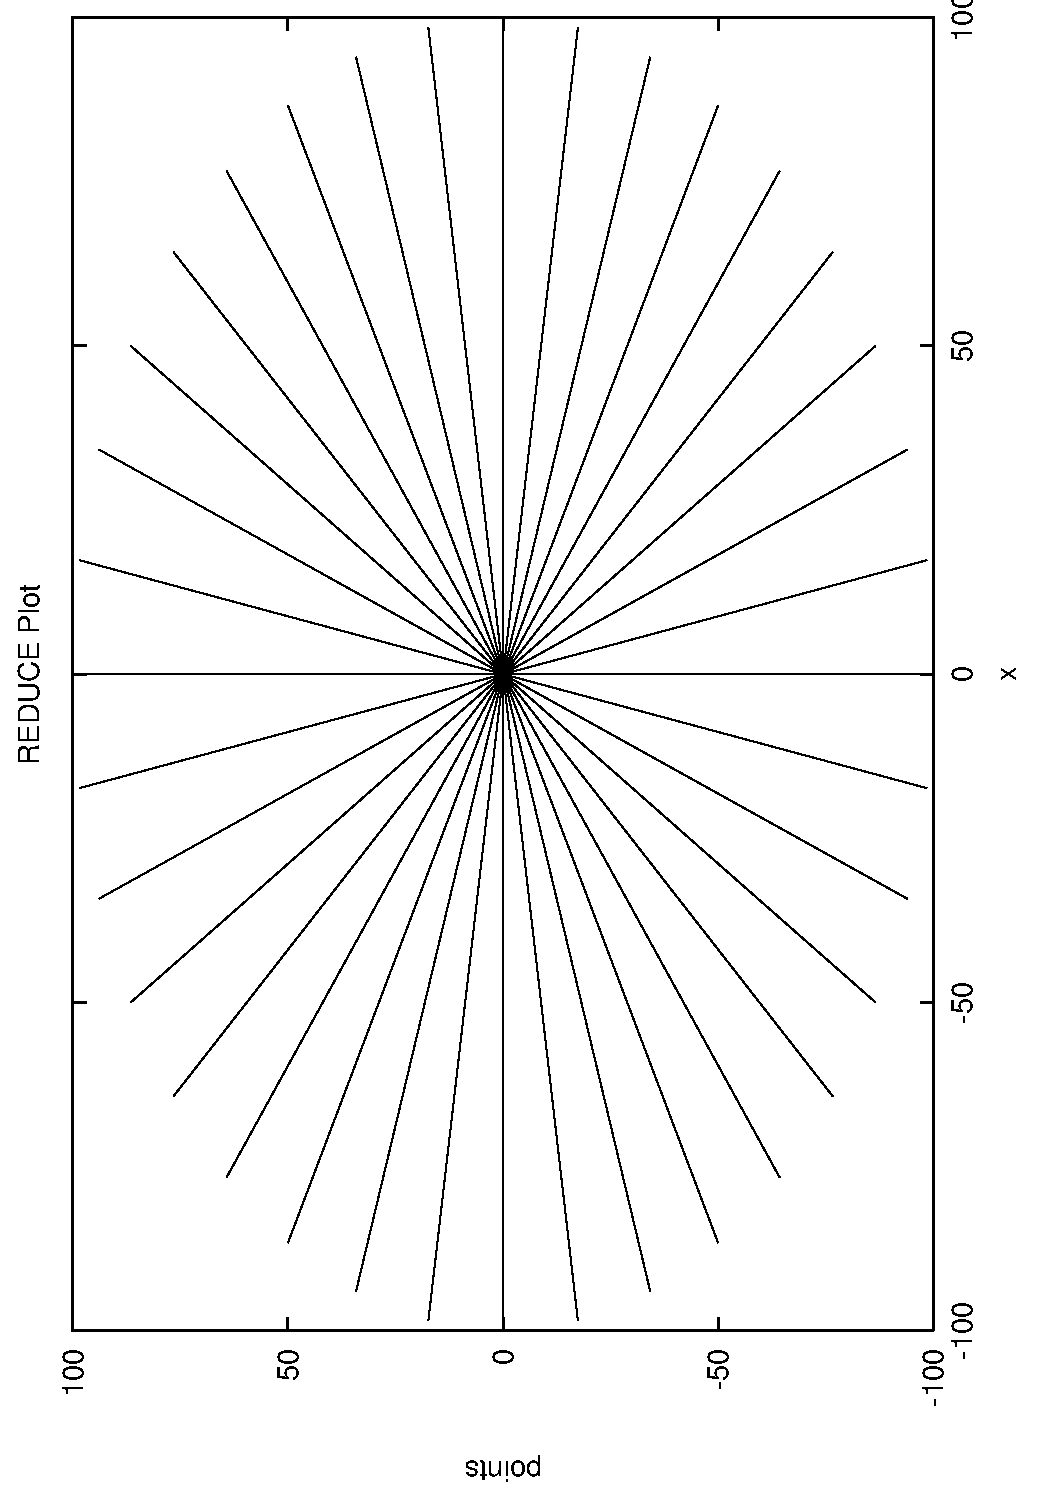
\includegraphics[bb=0 0 504 720,width=8cm,height=8cm,angle=270]{turtleeg1.pdf}}
\end{picture}

\begin{verbatim}
% (2) Draw 12 regular polygons with 12 sides of length 40,each polygon
%forming an angle of 360/n degrees with the previous one. 

draw {for i:=1:12 collect
          {leftturn(30), for j:=1:12 collect
                             {forward 40, leftturn(30)}} };
\end{verbatim}

\unitlength=1cm
\begin{picture}(8,8)(0,0)
\put (0,8){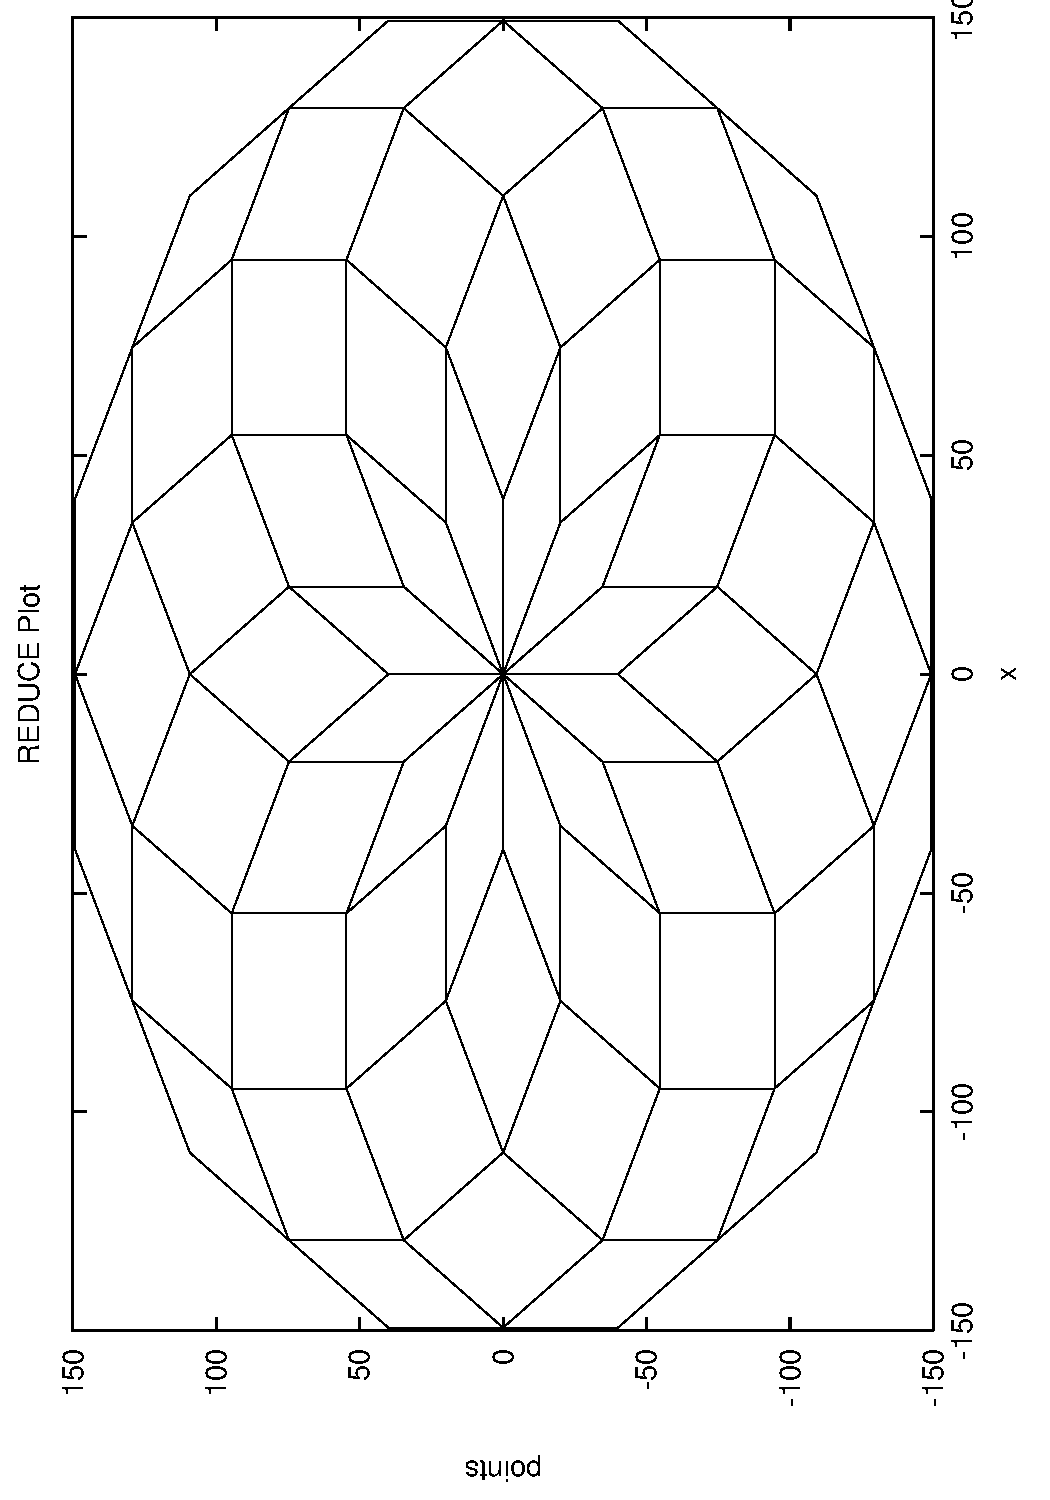
\includegraphics[bb=0 0 504 720,width=8cm,height=8cm,angle=270]{turtleeg4.pdf}}
\end{picture}

\begin{verbatim}
% (3) A "peak" pattern - an example of a recursive procedure.

procedure peak(r);
begin;
  return for i:=0:r collect
             {move(x_coord+5,y_coord-10), move(x_coord+10,y_coord+60),
              move(x_coord+10,y_coord-60),move(x_coord+5,y_coord+10)};
end;

draw {home(), peak(3)};
\end{verbatim}

\unitlength=1cm
\begin{picture}(8,8)(0,0)
\put (0,8){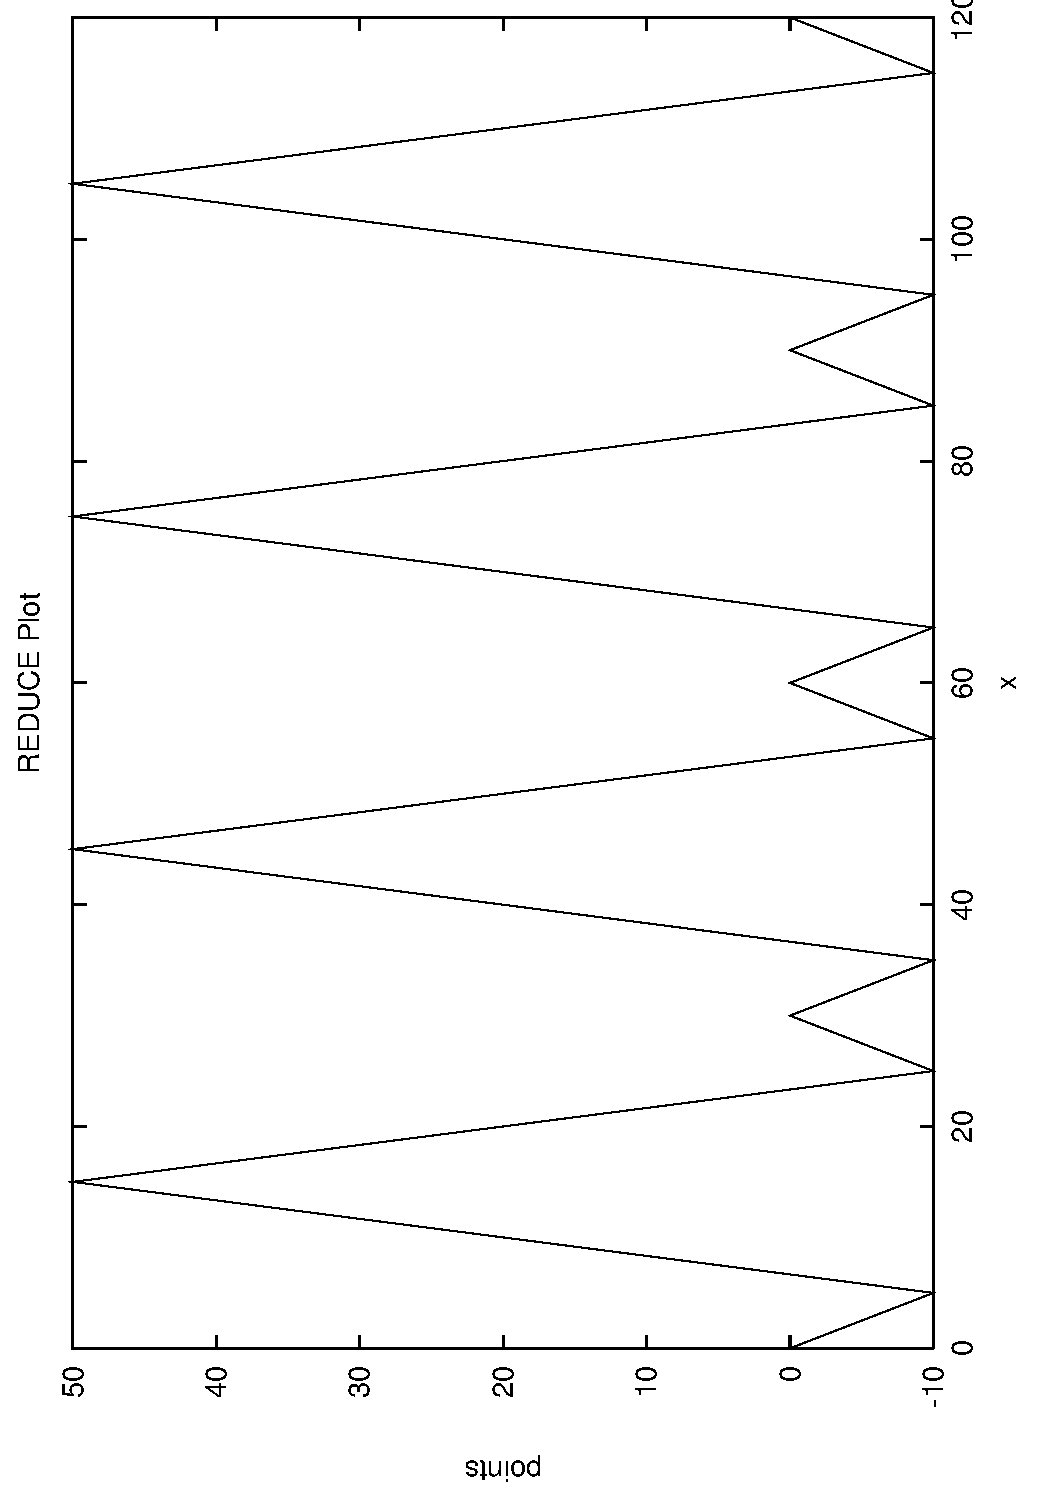
\includegraphics[bb=0 0 504 720,width=8cm,height=8cm,angle=270]{turtleeg5a.pdf}}
\end{picture}  

\begin{verbatim}
%This procedure can then be part of a longer chain of commands:

draw {home(), move(5,50), peak(3), move(x_coord+10,-100),
      peak(2), move(x_coord+10,0)};
\end{verbatim}

\unitlength=1cm
\begin{picture}(8,8)(0,0)
\put (0,8){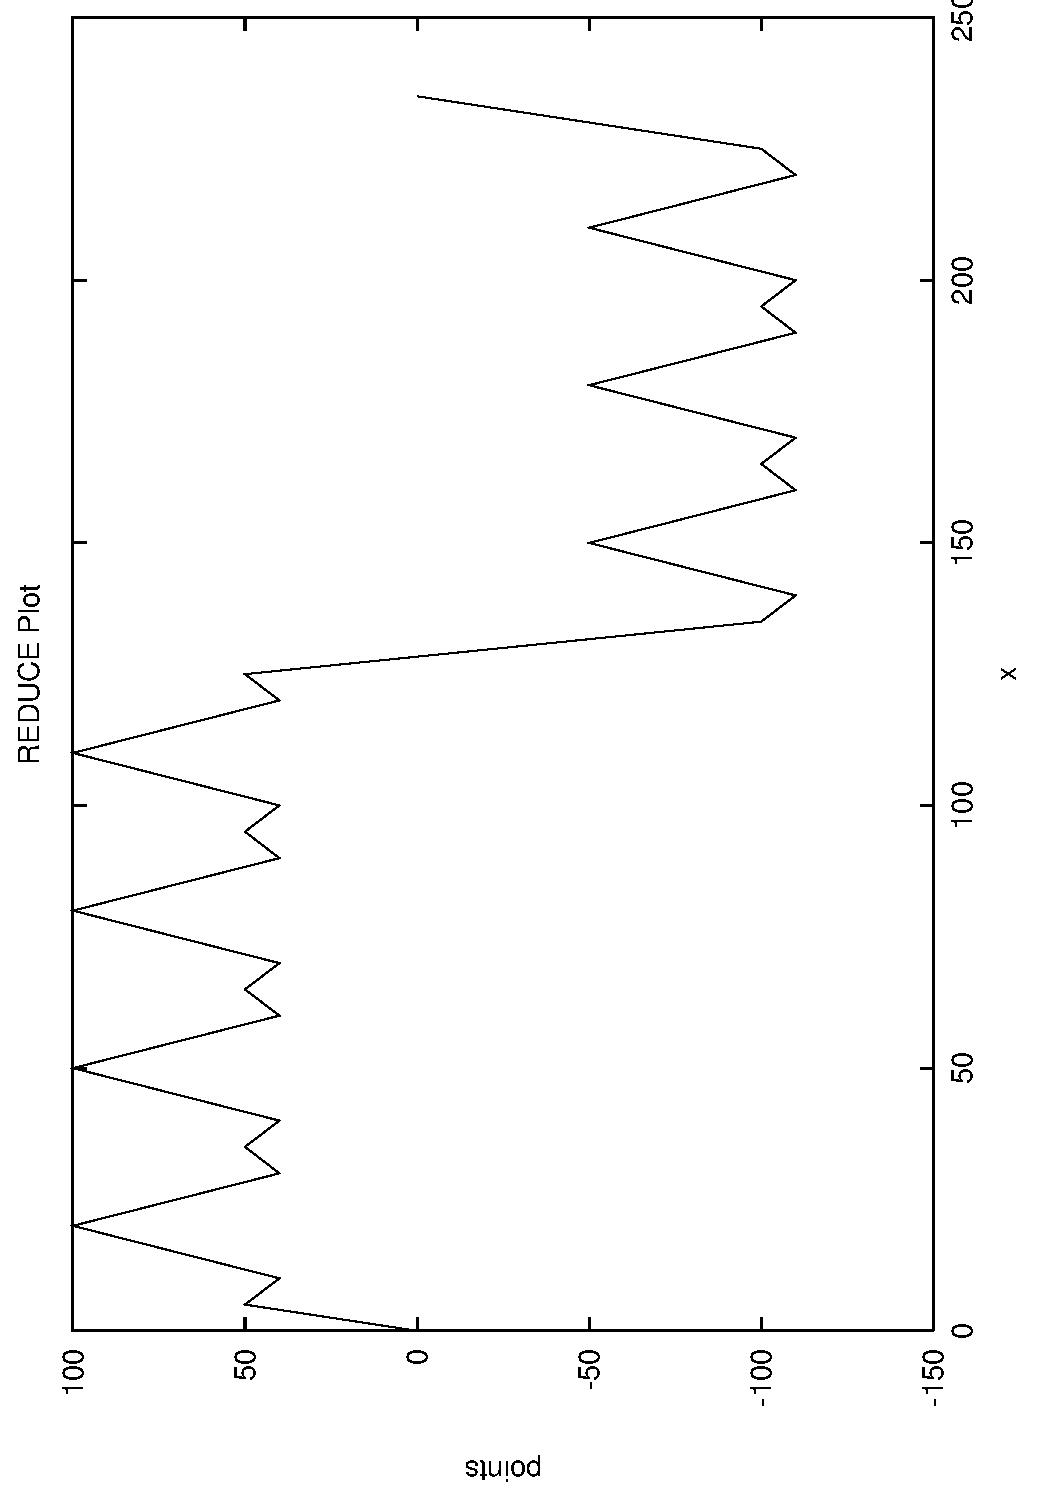
\includegraphics[bb=0 0 504 720,width=8cm,height=8cm,angle=270]{turtleeg5b.pdf}}
\end{picture}  

\begin{verbatim}
% (4)  Write a recursive procedure which draws "trees" such that every
%branch is half the length of the previous branch.

procedure tree(a,b);         %Here: a is the start length, b is the
                             %number of levels
begin;
  return if fixpb and b>0           %checking b is a positive integer

            then {leftturn(45), forward a, tree(a/2,b-1),
                  back a, rightturn(90), forward a, tree(a/2,b-1),
                  back a, leftturn(45)}
         else {x_coord,y_coord};    %default: Turtle stays still
end;

draw {home(), tree(130,7)};
\end{verbatim}

\unitlength=1cm
\begin{picture}(8,8)(0,0)
\put(0,8){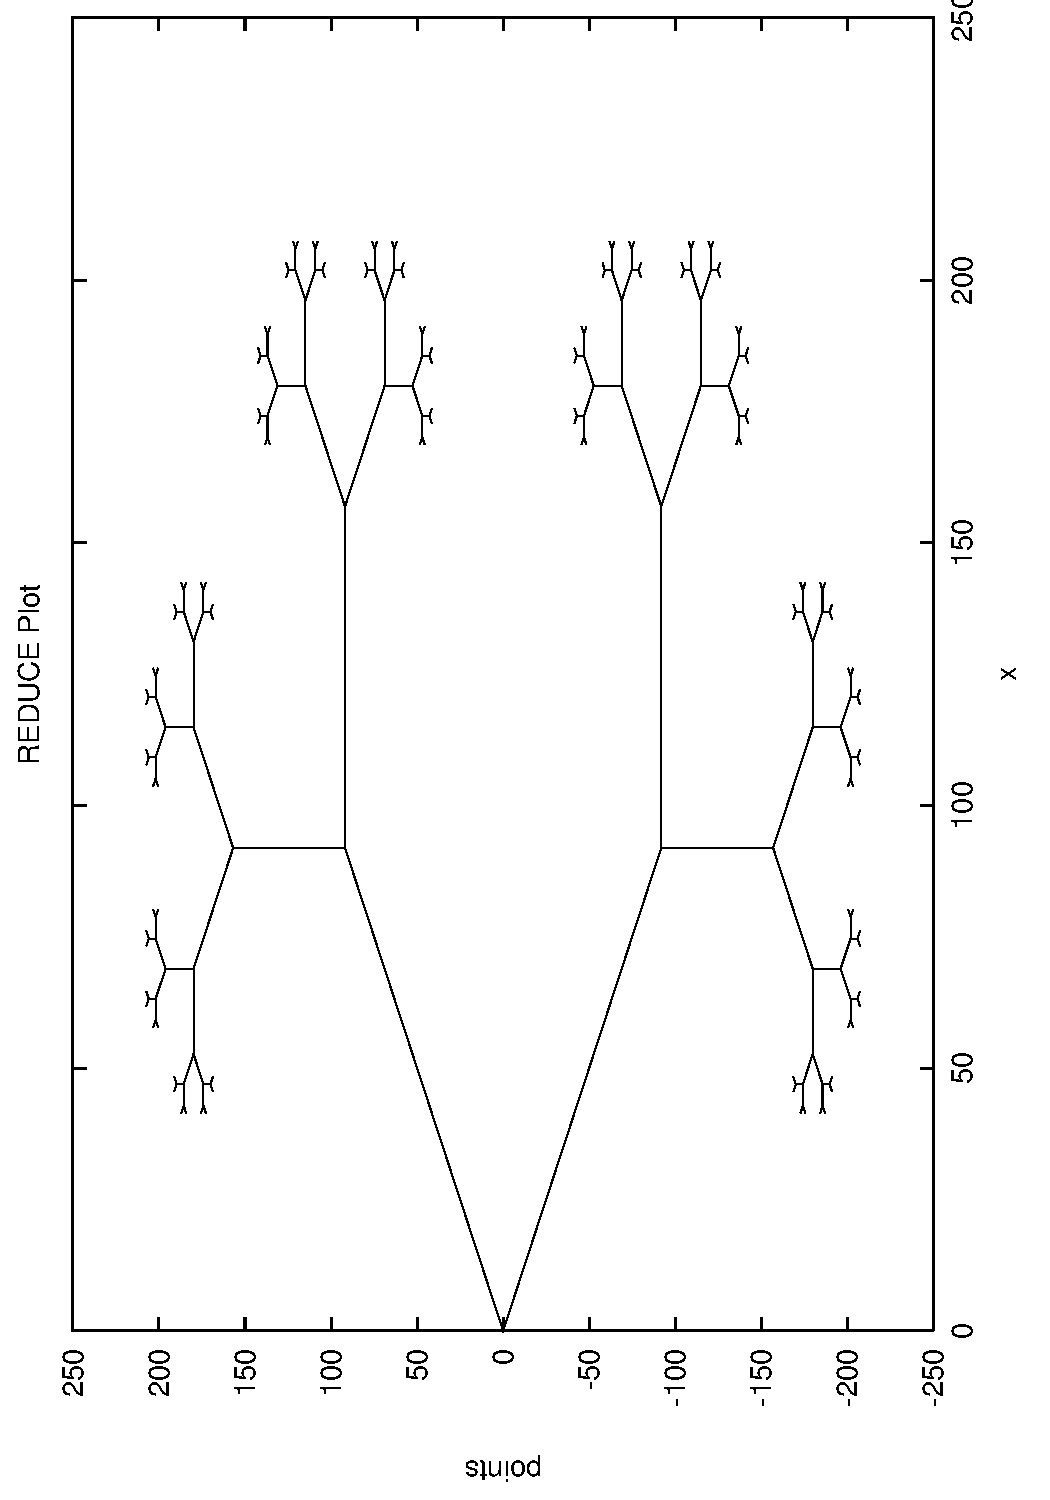
\includegraphics[bb=0 0 504 720,width=8cm,height=8cm,angle=270]{turtleeg6a.pdf}}
\end{picture}  

\begin{verbatim}
% (5)  A 36-point star.

draw {home(), for i:=1:36 collect
                  {leftturn(10), forward 100, leftturn(10), back 100} };
\end{verbatim}

\unitlength=1cm
\begin{picture}(8,8)(0,0)
\put(0,8){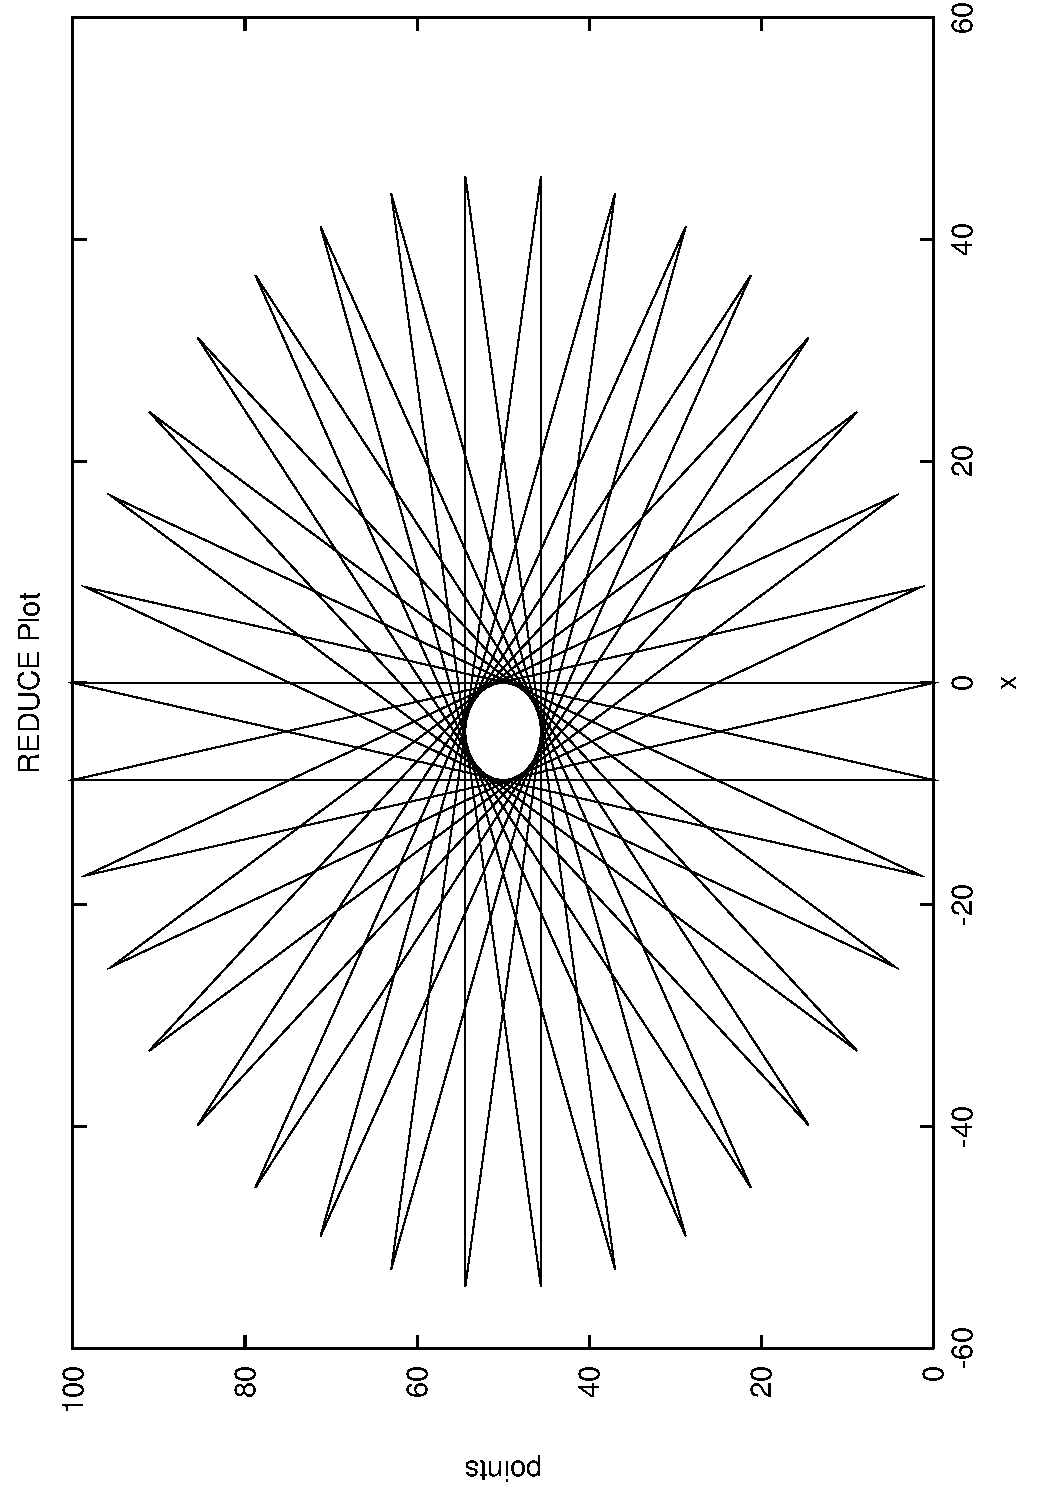
\includegraphics[bb=0 0 504 720,width=8cm,height=8cm,angle=270]{turtleeg7.pdf}}
\end{picture}  

\begin{verbatim}
% (6) Draw 100 equilateral triangles with the leading points
%equally spaced on a circular path.

draw {home(), for i:=1:100 collect
                  {forward 150, rightturn(60), back(150),
                   rightturn(60), forward 150, setheading(i*3.6)} };
\end{verbatim}

\unitlength=1cm
\begin{picture}(8,8)(0,0)
\put(0,8){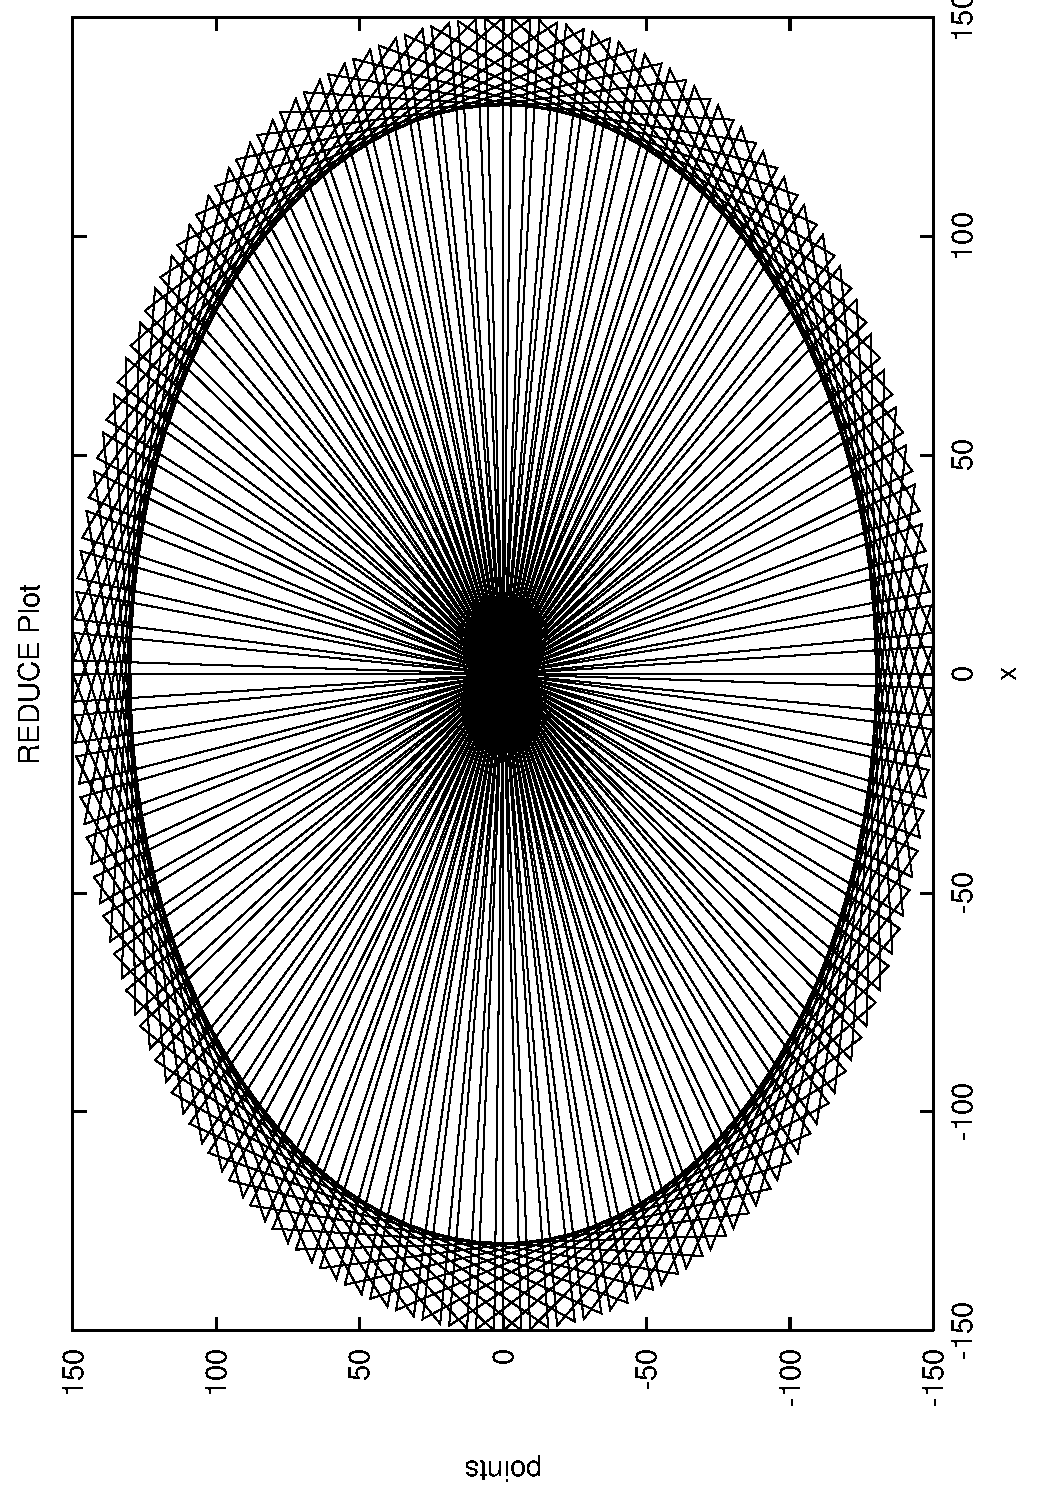
\includegraphics[bb=0 0 504 720,width=8cm,height=8cm,angle=270]{turtleeg8.pdf}}
\end{picture}  

\begin{verbatim}
% (7) Two or more graphs can be drawn together (this is easier
%if the graphs are named). Here we show graphs 2 and 6 on top of one
%another:

gr2:={home(), for i:=1:12 collect
                  {leftturn(30), for j:=1:12 collect
                                     {forward 40, leftturn(30)}} }$

gr6:={home(), for i:=1:100 collect
                  {forward 150, rightturn(60), back(150),
                   rightturn(60), forward 150, setheading(i*3.6)} }$

draw {gr2, gr6};
\end{verbatim}

\unitlength=1cm
\begin{picture}(8,8)(0,0)
\put(0,8){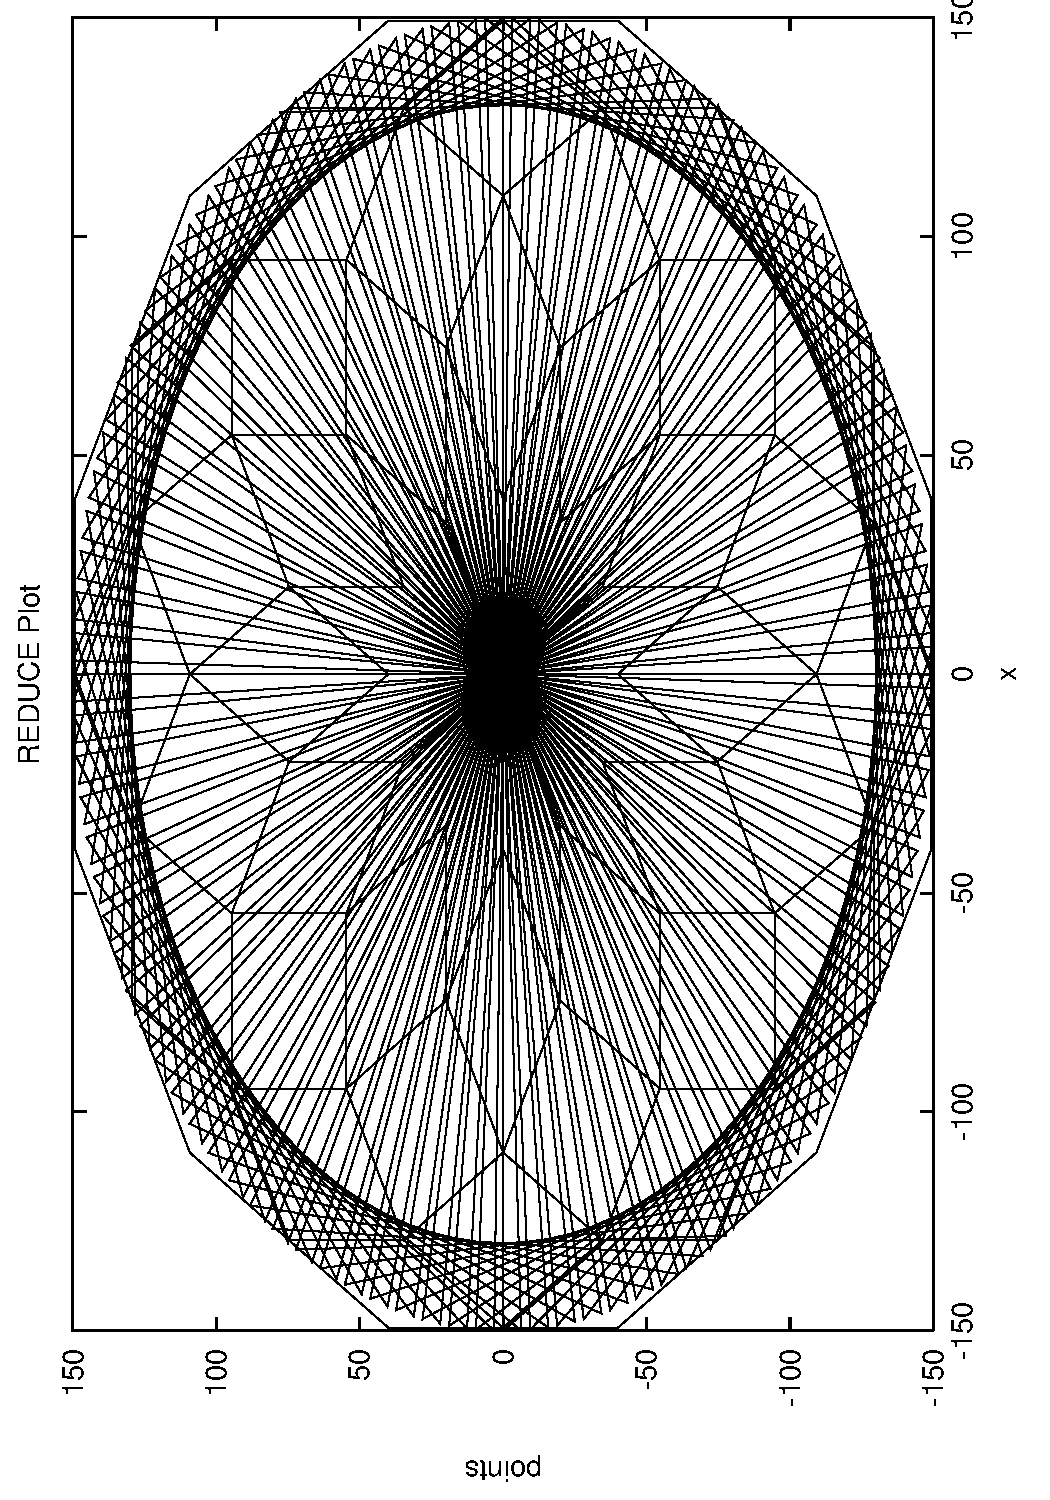
\includegraphics[bb=0 0 504 720,width=8cm,height=8cm,angle=270]{turtleeg9.pdf}}
\end{picture}  

\begin{verbatim}
% (8) Example 7 could have been tackled another way, which makes use of 
%the fdraw command.
%By inputting gr2 and gr6 as procedures into reduce, they can then be 
%used at any time in the same reduce session in a call to draw and even
%fdraw.

%First save the procedures in a file, say fxp (fdraw example procedures):

procedure gr2;
begin;
  return {home, for i:=1:12 collect
                    {leftturn(30), for j:=1:12 collect
                                       {forward 40, leftturn(30)}} };
end;

procedure gr6;
begin;
  return {home(), for i:=1:100 collect
                  {forward 150, rightturn(60), back(150),
                   rightturn(60), forward 150, setheading(i*3.6)} };
end;

%Then create another file where the functions may be called to fdraw,
%e.g. fx:

gr2
gr6

%Now in reduce, after loading the turtle package just type the following:

in "fxp";
fdraw '"fx";

%..and the graphs will appear.

%This method is useful if the user wants to define many of their own
%functions, and, using fdraw, subtle changes can be made quickly without 
%having to type out the whole string of commands to plot each time. It 
%is particularly useful if there are several pictures to plot at once and 
%it is an easy way to build pictures so that the difference an extra 
%command makes to the overall picture can be clearly seen.
%(In the above example, the file called to fdraw was only 2 lines long,
%so this method did not have any advantage over the normal draw command. 
%However, when the list of commands is longer it is clearly advantageous 
%to use fdraw)


\end{verbatim}


\subsection{References}

\begin{enumerate}
 \item {\bf An Implementation of Turtle Graphics for Teaching Purposes}\\
         Zoran I. Putnik \& Zoram d.Budimac

 \item {\bf Mapletech -} Maple in Mathematics and the Sciences,\\ 
        Special Issue 1994\\
       {\bf An Implementation of ``Turtle Graphics'' in Maple V}\\
         Eugenio Roanes Lozano \&  Eugenio Roanes Macias

\end{enumerate}






\newpage

\section{WU: Wu algorithm for polynomial systems} \ttindex{WU}

This is a simple implementation of the Wu algorithm implemented in REDUCE
working directly from ``A Zero Structure Theorem for
Polynomial-Equations-Solving,'' Wu Wen-tsun, Institute of Systems Science,
Academia Sinica, Beijing.

Author: Russell Bradford.

\section{XCOLOR: Color factor in some field theories}
\ttindex{XCOLOR}

This package calculates the color factor in non-abelian gauge field
theories using an algorithm due to Cvitanovich.

Documentation for this package is in plain text.

Author: A. Kryukov.

\section{XIDEAL: Gr\"obner Bases for exterior algebra} \ttindex{XIDEAL}

XIDEAL constructs Gr\"obner bases for solving the left ideal membership
problem: Gr\"obner left ideal bases or GLIBs. For graded ideals, where each
form is homogeneous in degree, the distinction between left and right
ideals vanishes. Furthermore, if the generating forms are all homogeneous,
then the Gr\"obner bases for the non-graded and graded ideals are
identical. In this case, XIDEAL is able to save time by truncating the
Gr\"obner basis at some maximum degree if desired.

Author: David Hartley.

\section{ZEILBERG: Indefinite and definite summation}
\ttindex{ZEILBERG}

This package is a careful implementation of the Gosper and Zeilberger
algorithms for indefinite and definite summation of hypergeometric terms,
respectively.  Extensions of these algorithms are also included that are
valid for ratios of products of powers, factorials, $\Gamma$ function
terms, binomial coefficients, and shifted factorials that are
rational-linear in their arguments.

Authors: Gregor St\"olting and Wolfram Koepf.

\section{ZTRANS: \texorpdfstring{$Z$}{\textit{Z}}-transform package}
\ttindex{ZTRANS}

This package is an implementation of the $Z$-transform of a sequence.
This is the discrete analogue of the Laplace Transform.

Authors: Wolfram Koepf and Lisa Temme.

\let\sectionmark=\origsectionmark
